\documentclass[a4paper]{scrreprt}

%%% PACKAGES %%%

%etoolbox for rules
\usepackage{etoolbox}

% Figure Placement
\usepackage{float}
% PDF/A Compliance
%\usepackage[a-2b,latxmp]{pdfx}

% add Unicode support and use English as language
\usepackage[utf8]{inputenc}
\usepackage[english]{babel}

% Use Times NR as font
\usepackage{lmodern}
\usepackage[T1]{fontenc}

% Better tables
\usepackage{tabularx}

% Better enumerisation env
\usepackage{enumitem}
\usepackage{multirow}

% Use graphics
\usepackage{graphicx}

% Have subfigures and captions
\usepackage{subcaption}

% Be able to include PDFs in the file
\usepackage{pdfpages}

% Have custom abstract heading
\usepackage{abstract}

% Need a list of equation
\usepackage{tocloft}
\usepackage{ragged2e}

\usepackage{dirtree}
\usepackage{adjustbox}

% Better equation environment
\usepackage{amsmath}

% Symbols for most SI units
\usepackage{siunitx}

\usepackage{csquotes}

% to make beautiful tables
\usepackage{booktabs}

% Clickable Links to Websites and chapters
\usepackage[hidelinks]{hyperref}

% New command for 'fullref'
\newcommand*{\fullref}[1]{\hyperref[{#1}]{\nameref*{#1} (\ref*{#1})}}

% lscape.sty Produce landscape pages in a (mainly) portrait document.
%\usepackage{lscape}
\usepackage{pdflscape}

% Symbols like checkmark
\usepackage{amssymb}
\usepackage{pifont}

% Lorem ipsum package for default text
\usepackage{lipsum}

\usepackage[absolute]{textpos}

\usepackage{longtable}

% Header
\usepackage{scrlayer-scrpage}

\clearpairofpagestyles

% sets the font of the document headers to Times NR
\addtokomafont{disposition}{\rmfamily}

 % Configures header and footer
\setkomafont{pageheadfoot}{\rmfamily\footnotesize}
\setkomafont{pagehead}{\rmfamily\bfseries}
\setkomafont{pagination}{}

% Displays line for header and footer
\KOMAoptions{
   headsepline = true,
   footsepline = true,
   plainfootsepline = true,
}

\usepackage{tikz}
\tikzset{
    input/.style = {coordinate},
    output/.style = {coordinate},
    block/.style={rectangle, draw, text width=7.3em,
           text centered, rounded corners, minimum height=3em},
    arrow/.style={-{Stealth[]}}
     }
\usetikzlibrary{positioning,arrows.meta}

\usepackage{pgfgantt}
\usepackage{graphicx}
\usepackage{xcolor}

\ganttset{group/.append style={orange},
milestone/.append style={red},
progress label node anchor/.append style={text=red}}

\automark[chapter]{chapter}

\ohead{\headmark}
\ihead{Fabian Gröger}

\ofoot*{\pagemark}
\ifoot*{HSLU BAA - Deep embedded Music}

% Glossary, hyperref, babel, polyglossia, inputenc, fontenc must be loaded before this package if they are used
\usepackage[ 
xindy,
toc,         
acronym,
nopostdot,
sort=standard   
]{glossaries}

\setglossarystyle{listgroup}

% Redefine the quote charachter as we are using ngerman
%\GlsSetQuote{+}
% Define the usage of an acronym, Abbreviation (Abbr.), next usage: The Abbr. of ...
\setacronymstyle{long-short}

% Bibliography & citing
\usepackage[
	backend=biber,
	style=authoryear,
	bibstyle=authoryear,
	citestyle=authoryear
	]{biblatex}
\addbibresource{references_zotero.bib}
\addbibresource{Referenzen.bib}
\addbibresource{Links.bib}
\DeclareLanguageMapping{english}{english-apa}

%%% COMMAND REBINDINGS %%%
\newcommand{\tabitem}{~~\llap{\textbullet}~~}
\newcommand{\xmark}{\ding{55}}
\newcommand{\notmark}{\textbf{\textasciitilde}}
% Pro/Con item https://tex.stackexchange.com/questions/145198/change-the-bullet-of-each-item#145203
\newcommand\pro{\item[$+$]}
\newcommand\con{\item[$-$]}

% Define list of equations - Thanks to Charles Clayton: https://tex.stackexchange.com/a/354096
\newcommand{\listequationsname}{List of Equations}
\newlistof{myequations}{equ}{\listequationsname}
\newcommand{\myequations}[1]{
	\addcontentsline{equ}{myequations}{\protect\numberline{\theequation}#1}
}
\setlength{\cftmyequationsnumwidth}{2.3em}
\setlength{\cftmyequationsindent}{1.5em}

% Usage {equation}{caption}{label}
\newcommand{\indexequation}[3]{
	\begin{align} \label{#3} \ensuremath{#1} \end{align}
	\myequations{#3} \centering #2 \normalsize \justify }
	
% equations with term definitions, credit to tex.stackexchange.com/questions/95838/how-to-write-a-perfect-equation-parameters-description
\newenvironment{conditions}
  {\par\vspace{\abovedisplayskip}\noindent\begin{tabular}{>{$}l<{$} @{${}={}$} l}}
  {\end{tabular}\par\vspace{\belowdisplayskip}}
  
\newenvironment{conditions*}
  {\par\vspace{\abovedisplayskip}\noindent
   \tabularx{\columnwidth}{>{$}l<{$} @{${}={}$} >{\raggedright\arraybackslash}X}}
  {\endtabularx\par\vspace{\belowdisplayskip}}

% Todolist - credit to https://tex.stackexchange.com/questions/247681/how-to-create-checkbox-todo-list
\newlist{todolist}{itemize}{1}
\setlist[todolist]{label=$\square$}

% Nested Enumeratelist credit to https://tex.stackexchange.com/a/54676
\newlist{legal}{enumerate}{10}
\setlist[legal]{label*=\arabic*.}

% Formatting Chapter title, thanks to: 
% http://texnorte.blogspot.com/2012/06/insert-code-before-chapter-title.html
\newcommand\toptitle{}
\makeatletter
\def\@makechapterhead#1{%
  \vspace*{50\p@}%
  {\parindent \z@ \raggedright \normalfont
    \ifnum \c@secnumdepth >\m@ne
      \if@mainmatter
        \toptitle\par
        \huge\bfseries \@chapapp\space \thechapter
        \par\nobreak
        \vskip 20\p@
      \fi
    \fi
    \interlinepenalty\@M
    \Huge \bfseries #1\par\nobreak
    \vskip 40\p@
  }}
\makeatother

%%% GLOSSARY %%%
%%% ACRONYM ENTRIES %%%
\newacronym{DSP}{DSP}{Digital Signal Processing}
\newacronym{ADC}{ADC}{Analog-to-Digital converter}
\newacronym{DAC}{DAC}{Digital-to-Analog converter}
\newacronym{ASR}{ASR}{Automatic Speech Recognition}
\newacronym{ML}{ML}{Machine Learning}
\newacronym{NN}{NN}{Neuronales Netz}
\newacronym{KNN}{KNN}{Künstliches neuronales Netz}
\newacronym{ANN}{ANN}{Artificial Neuronal Net}
\newacronym{CNN}{CNN}{Convolutional Neural Network}
\newacronym{RNN}{RNN}{Recurrent neural network}
\newacronym{LSTM}{LSTM}{Long short term memory}
\newacronym{GAN}{GAN}{Generative Adversarial Networks}
\newacronym{VAE}{VAE}{Variational Auto-Encoder}
\newacronym{RAM}{RAM}{Random Access Memory}
\newacronym{TPU}{TPU}{Tensor processing unit}
\newacronym{GPU}{GPU}{Graphics processing unit}
\newacronym{Hz}{Hz}{Hertz}
\newacronym{kHz}{kHz}{Kilohertz}
\newacronym{SINS}{SINS}{Sound Interfacing through the Swarm}
\newacronym{DCASE}{DCASE}{Detection and Classification of Acoustic Scenes and Events}
\newacronym{AAL}{AAL}{Ambient Assisted Living}
\newacronym{MFCC}{MFCC}{Mel Frequency Cepstral Coefficients}
\newacronym{FT}{FT}{Fourier Transform}
\newacronym{FFT}{FFT}{Fast Fourier Transformation}
\newacronym{DFT}{DFT}{Discrete Fourier Transformation}
\newacronym{DCT}{DCT}{Discrete Cosine Transformation}
%%% GLOSSARY ENTRIES %%%
\newglossaryentry{Epoche}{name=Epoche, description={Kompletter Durchlauf aller Input-Daten}}
\newglossaryentry{Batch}{name=Batch, description={Anzahl der Input-Daten bevor die Parameter angepasst werden}}
\newglossaryentry{controlgen}{name=ControlGen, description={Das ControlGen Style Transfer Modell}}
\newglossaryentry{crossalign}{name=CrossAlign, description={Das CrossAlign Style Transfer Modell}}

\makeglossaries

%%% PATH DEFINITIONS %%%
% Define the path were images are found
\graphicspath{{./img/}{./appendix/}}

% Reset Glossary every chapter
\preto\chapter{\glsresetall}

%%%%%%%%%%%%%%%%
%%% DOCUMENT %%%

\begin{document}

% HSLU Preamble (no header or footer)
\pagestyle{empty}

% Cover Page
\begin{titlepage}
	\begin{textblock*}{5cm}[0,0](15.1cm,0.7cm)
		
\includegraphics[keepaspectratio,width=5cm]{img/HSLU_Logo}
	\end{textblock*}
	\begin{center}
		\vspace*{5cm}
		\Huge{\textbf{Deep Embedded Music}} \\
		\vspace{0.5em}
		\LARGE{\textsc{Bachelor Thesis}}\\
		\vspace{2em}
		\Large{presented by}\\
		\LARGE{\textsc{Fabian Gröger}}\\
		\vspace{2em}
		\Large{Departement Information Technology}\\
		\Large{Lucerne University of Applied Sciences and Arts}\\
		\Large{6343 Rotkreuz, Switzerland}\\
		\vspace{4em}
		\Large{\today}\\
		\vfill
		\begin{center}
		\resizebox{\textwidth}{!}{%
        \begin{tabular}{ l l }
         Advisor: & Daniel Pfäffli \\ 
         \ & Lucerne University of Applied Sciences and Arts, 6343 Rotkreuz, Switzerland \\
         \ & daniel.pfaeffli@hslu.ch \\ 
         Expert: & TBD
        \end{tabular}}
        \end{center}
	\end{center}
	\begin{textblock*}{5cm}[0,0](15.3cm,277mm)
		
\includegraphics[keepaspectratio,width=5cm]{img/FHZ_Logo}
	\end{textblock*}
\end{titlepage}

\newpage
\pagenumbering{gobble}

\begin{textblock*}{5cm}[0,0](15cm,0.7cm)
	
\includegraphics[keepaspectratio,width=2.7cm]{img/HSLU_Logo_Header}
\end{textblock*}

\vspace{0.6cm}
\noindent
\textbf{\Large{Bachelorarbeit an der Hochschule Luzern – Informatik}}

\vspace{0.6cm}
\noindent
\textbf{Titel:} Deep Embedded Music

\vspace{0.6cm}
\noindent
\textbf{Studentin / Student:} Fabian Gröger

\vspace{0.6cm}
\noindent
\textbf{Studiengang:} BSc Informatik

\vspace{0.6cm}
\noindent
\textbf{Abschlussjahr:} 2020

\vspace{0.6cm}
\noindent
\textbf{Betreuungsperson:} Daniel Pfäffli, HSLU Informatik, Rotkreuz

\vspace{0.6cm}
\noindent
\textbf{Expertin / Experte:} Dr. Jeremy Callner, APG/SGA, Zürich

\vspace{0.6cm}
\noindent
\textbf{Auftraggeberin / Auftraggeber:} Hochschule Luzern - Informatik

\vspace*{1.00cm}

\noindent
\textbf{Codierung / Klassifizierung der Arbeit:} Innovationsprojekte (Projekte mit
Erkenntnisgewinn, Forschungsprojekte)

\begin{todolist}
	\item \textbf{A: Einsicht (Normalfall)}
	\item \textbf{B: Rücksprache}\hspace*{0.7cm}(Dauer:\hspace*{1cm} Jahr / Jahre)
	\item \textbf{C: Sperre}\hspace*{1.865cm}(Dauer:\hspace*{1cm} Jahr / Jahre)
\end{todolist}

\vspace*{1.00cm}

\noindent
\textbf{Eidesstattliche Erklärung}
\\
Ich erkl\"are hiermit, dass ich/wir die vorliegende Arbeit selbst\"andig und ohne unerlaubte fremde Hilfe angefertigt haben, alle verwendeten Quellen, Literatur und andere Hilfsmittel angegeben haben, w\"ortlich oder inhaltlich entnommene Stellen als solche kenntlich gemacht haben, das Vertraulichkeitsinteresse des Auftraggebers wahren und die Urheberrechtsbestimmungen der Fachhochschule Zentralschweiz (siehe Merkblatt <<Studentische Arbeiten>> auf MyCampus) respektieren werden.

\vspace{2em}

\noindent
\begin{tabularx}{\textwidth}{@{}lX}
	&\\
	Ort / Datum, Unterschrift: &  \\
	\cline{2-2}
\end{tabularx}

\begin{textblock*}{5cm}[0,0](14.93cm,277mm)
	
\includegraphics[keepaspectratio,width=5cm]{img/FHZ_Logo}
\end{textblock*}

\newpage

\begin{textblock*}{5cm}[0,0](15cm,0.7cm)
	
\includegraphics[keepaspectratio,width=2.7cm]{img/HSLU_Logo_Header}
\end{textblock*}

\noindent
\textbf{Abgabe der Arbeit auf der Portfolio Datenbank:}\\
Best\"atigungsvisum Studentin/Student\\
Ich best\"atige, dass ich die Bachelorarbeit korrekt gem\"ass Merkblatt auf der Portfolio Datenbank abgelegt habe. Die Verantwortlichkeit sowie die Berechtigungen habe ich abgegeben, so dass ich keine \"Anderungen mehr vornehmen kann oder weitere Dateien hochladen kann. \newline \newline 
Ort / Datum, Unterschrift	\underline{\hspace*{10cm}} \newline \newline \newline

\noindent
\textbf{Verdankung}\\
An dieser Stelle möchte ich mich recht herzlich bei meinem Betreuer, Daniel Pfäffli, bedanken, der mich während der ganzen Durchführung unterstützt und motiviert hat. Ich habe von ihm und seinem grossen Wissen enorm profitiert und wurde dadurch angetrieben mehr zu leisten. Ausserdem möchte ich mich herzlich bei Emanuel Oehri bedanken, der sich Zeit genommen hat, das Musik Data Set bereitzustellen und mit mir die qualitative Analyse durchzuführen. Weiter möchte ich mich bei meiner Frau Deborah Gröger bedanken für die Unterstützung über die ganze Dauer der Arbeit. Meinen Eltern Dr. Ulrich Gröger und Madeleine Gröger möchte ich meinen grössten Dank aussprechen für die konstante Unterstützung über die ganze Studienzeit.
\newline \newline \newline

\vspace{0.8cm}
\noindent
\textbf{Ausschliesslich bei Abgabe in gedruckter Form: \\ 
Eingangsvisum durch das Sekretariat auszufüllen}

\noindent
\renewcommand{\arraystretch}{2}
\begin{tabularx}{\textwidth}{@{}lXlX}
	Rotkreuz, den & & Visum: & \\
	\cline{2-2}
	\cline{4-4}
\end{tabularx}
\renewcommand{\arraystretch}{1}

\vfill
\noindent
{\textbf{Hinweis}}: Die Bachelorarbeit wurde von keinem Dozierenden nachbearbeitet. Ver\"offentlichungen (auch auszugsweise) sind ohne das Einverst\"andnis der Studiengangleitung der Hochschule Luzern -- Informatik nicht erlaubt. \newline \newline
Copyright \textcopyright\ {2020} Hochschule Luzern -- Informatik \newline \newline
Alle Rechte vorbehalten. Kein Teil dieser Arbeit darf ohne die schriftliche Genehmigung der Studiengangleitung der Hochschule Luzern -- Informatik in irgendeiner Form reproduziert oder in eine von Maschinen verwendete Sprache \"ubertragen werden.


\begin{textblock*}{5cm}[0,0](14.93cm,277mm)
	
\includegraphics[keepaspectratio,width=5cm]{img/FHZ_Logo}
\end{textblock*}


% Rest of the document has header and footer
\pagestyle{headings}
\pagenumbering{Roman}

% Abstract
\begin{abstract}
	\noindent
	\lipsum[50]
\end{abstract}

% Table of contents
\tableofcontents

\clearpage
\pagenumbering{arabic}

\chapter{Introduction}
\label{ch:Introduction}
This chapter aims to introduce the thesis \flqq Deep embedded Music\frqq \ and describes the task and the objectives of the project in detail. It should give an insight into the situation it arose from, as well as the motivation behind it. The detailed task, which was submitted to the Transfer Office of the Lucerne University of Applied Sciences and Arts, can be found in the appendix \fullref{app:Task-Definition}.

\section{Initial situation}
\label{sub:Initial-Stituation}
The last few years have seen significant advances in non-speech audio processing, as popular deep learning architectures, developed in the speech and image processing communities, have been ported to this relatively understudied domain. However, these data-hungry neural networks are not always matched to the available training data in the audio domain. While unlabeled audio is easy to collect, manually labelling data for each new sound application remains notoriously costly and time-consuming. Therefore a considerable amount of research in recent years focuses on the application of unsupervised machine learning in the audio domain.
\newline
\newline
When listening to music, distinguishing between music genres is for humans, from easy to difficult, depending on how similar the given genres are. It is rather simple to distinguish music songs, for example, of classical music and techno or country and hip-hop rap. However, the difficulty increases when songs within the same genre will need to be compared. When it comes to finding the similarity between songs or to sort a list of songs by their similarity, even humans fail to succeed. 
\newline
\newline
This thesis seeks to alleviate this problem by developing an alternative learning strategy that exploits basic semantic properties of sound that are not grounded by an explicit label. This alternative will then be applied to a noise detection dataset and a music dataset to show the applicability and performance of the approach. Further, it attempts to show that the representation learned, provides a similarity space for both datasets, which can then be used to compare specific audios, sort them by similarity or find similarities between categories.

\section{Task definition}
\label{sub:Task-Definition}
The goal of this thesis is to adapt Tile2Vec, an image embedding method, to audio streams and evaluate its performance on the noise detection dataset \flqq SINS, DCASE 2018: task 5\frqq. 
\newline
\newline
To achieve this goal, a model, which transforms the audio signals into embeddings, needs to be trained first. Then to evaluate the performance on the DCASE dataset, a simple classifier will be used, which receives an embedding and classifies it into one of the given classes within the dataset. The light classifier will be trained, and the accuracy of the resulting architecture will be compared to the published results of the DCASE 2018 Task 5 challenge.
\newline
\newline
This method is to be applied exploratively to different kinds of music, whereby a data set of 18h DJ music is available. The resulting clusters will be investigated qualitatively, by using clustering techniques as well as manual evaluation.

\section{Target setting}
\label{sub:Target-Setting}
As stated in \fullref{sub:Task-Definition}, the goal of the thesis is to adapt Tile2Vec to audio streams and evaluate its performance. Because this task was never done before, the thesis is categorised as an exploratory innovation/research project. The target is also to give some overview of how advanced the current research is in the section of unsupervised machine learning with audio and also give some outlook on further projects to explore different approaches.

\section{Preliminaries}
\label{sub:Preliminaries}
The focus of the thesis is exclusively on the architecture of the embedding model and the preprocessing of the audio signal. Clustering and classification are explicitly excluded from the research. Instead, proven and established standard approaches are to be used.
\newline
\newline
Clustering will only be used for evaluating the resulting clusters within the embedding space of the music dataset. For the classification, a simple two-layered dense model is used and should only to give some insights on how well a simple model performs on the resulting embedding space. The idea is to show that there is a specific performance gain when using the embedding space.
\newline
\newline
Optimization methods for training neural networks are explicitly excluded from the research. Instead, state-of-the-art techniques implemented in Tensorflow are used.


\chapter{Related Work}
\label{ch:Related-Work}
This chapter introduces and explains terms and concepts used throughout the thesis. Thus, this section can be used as a reference guide to fill in any gaps and to understand the relationships between the individual concepts better.

\section{Introduction to Digital Signal Processing}
\label{sec:Intro-DSP}
This section introduces the fundamentals of \gls{DSP}, which will be used repeatedly in the following sections, either to describe some behaviour or to reason. 
\newline
\newline
What exactly is \gls{DSP}? \gls{DSP} is to take real-world signals like voice, audio, video, temperature, pressure, or position that have been digitized and mathematically manipulate them. A \gls{DSP} is designed for performing mathematical functions such as \textit{add}, \textit{subtract}, \textit{multiply} and \textit{divide} very quickly.
\newline
\newline
Signals need to be processed so that the information that they contain can be displayed, analyzed, or converted to another type of signal that may be of use. In the real-world, analogue products detect signals such as sound, light, temperature or pressure and manipulate them. Converters such as an \gls{ADC} then take the real-world signal and turn it into the digital format of \texttt{1}'s and \texttt{0}'s. From here, the \gls{DSP} takes over by capturing the digitized information and processing it. It then feeds the digitized information back for use in the real world. It does this in one of two ways, either digitally or in an analogue format by going through a \gls{DAC}. All of this occurs at very high speeds.\footnotemark
\footnotetext{\href{https://www.analog.com/en/design-center/landing-pages/001/beginners-guide-to-dsp.html}{analog.com/en/design-center/landing-pages/001/beginners-guide-to-dsp.html}}

\subsection{Waveform}
\label{sub:Waveform}
Speech signals are sound signals, which are defined as pressure variations travelling through the air. These variations in pressure can be described as waves, and are therefore often called sound waves. In the current thesis, the focus is on the analysis and processing of such waveforms in digital systems. Therefore it is always assumed that the acoustic speech signals have been captured by a microphone and converted to a digital form.
\newline
\newline
A speech signal of finite length can be represented by a digitalised finite-length sequence $x[n]$, with $n = 0, 1, \dots, N-1$.

\subsection{Amplitude}
\label{sub:Amplitude}
The amplitude of a periodic variable is the measure of how far, and in what direction, that variable differs from zero. Thus, signal amplitudes can be either positive or negative. If the amplitude of a given signal is large, the signal is observed to be loud. Equation \ref{eq:Wave-Equation} shows a simple form of a wave equation, where $y$ is the oscillating variable (signal), $A$ the amplitude, $\gamma$ the period, $t$ the time and $\phi$ the phase shift. $sin(t)$ has a period of $2 \phi$. Figure \ref{fig:Amplitude-Wavelenght} illustrates such a simple wave form. 
\myequations{Simple wave equation}
\begin{equation}
    \centering
    y(t) = A \ sin(\gamma \ t + \phi)
    \label{eq:Wave-Equation}
\end{equation}
The distance from the top of one peak to the bottom of another is called \textit{peak-to-peak amplitude}. Another way to describe peak-to-peak amplitude is to say that it is the distance between the maximum positive value and the maximum negative value of a wave. In figure \ref{fig:Amplitude-Wavelenght}, the peak-to-peak amplitude of the wave would be $2A$.

\subsection{Magnitude}
\label{sub:Magnitude}

The magnitude of a periodic variable is the measure of how far, regardless of direction, its quantity differs from zero. So magnitudes are always positive values. Occasionally, in the literature of digital signal processing, the term magnitude is referred to as the absolute value. In figure \ref{fig:Amplitude-Wavelenght}, the magnitude of the wave would be $|A|$.

\subsection{Period}
\label{sub:Period}

The period is the length of a single cycle of a wave, as measured by the distance between one peak of a wave and the next. In figure \ref{fig:Amplitude-Wavelenght}, the wavelength is denoted as the variable $\gamma$. But not every signal is periodic, only if the signal satisfies the condition $\gamma = 2k\pi$ where $k \in \mathbb{Z}$.

\subsection{Frequency}
\label{sub:Frequency}

Frequency is the number of occurrences of a repeating event per unit of time. It depends on the wavelength of an audio signal $\lambda$. The frequency is given by the equation \ref{eq:Frequency}. If the signal at a given time has a high frequency, it is observed to have a higher pitch.

\myequations{Calculate frequency from wavelength}
\begin{equation}
    \centering
    f = \frac{1}{\gamma}
    \label{eq:Frequency}
\end{equation}

% TODO change image to notation used in equation!
\begin{figure}[htbp]
	\centering
	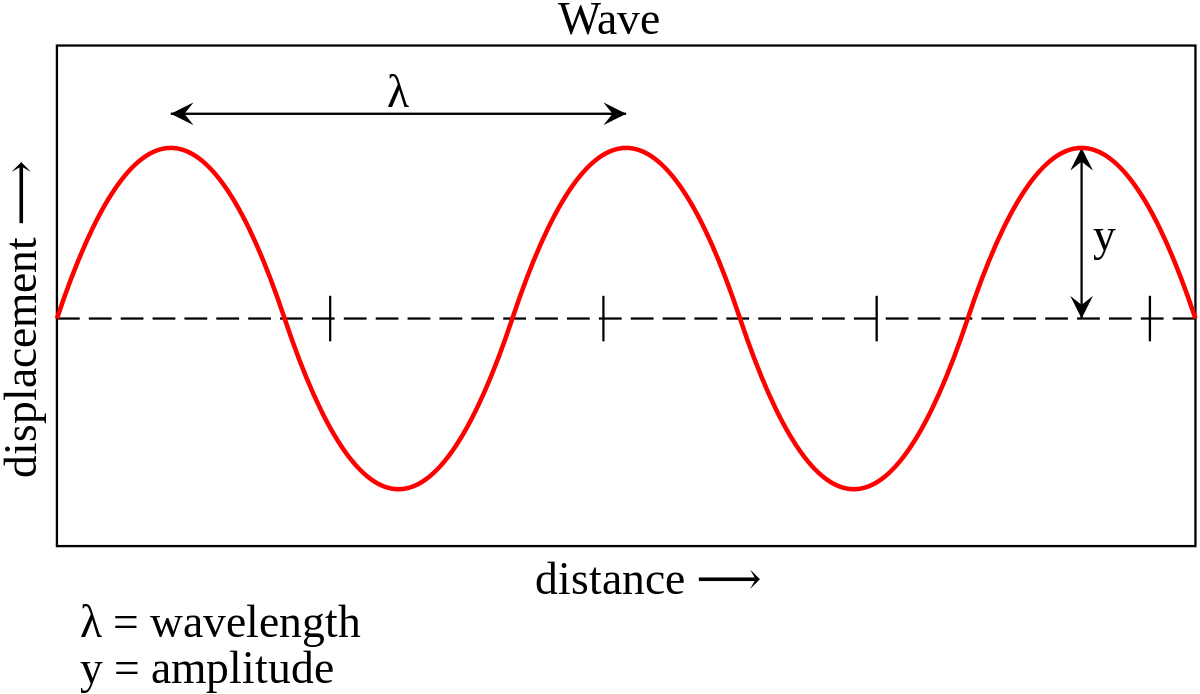
\includegraphics[scale=0.25]{img/Amplitude.png}
	\caption[Amplitude and wavelength illustrated]{Amplitude and wavelength \footnotemark}
	\label{fig:Amplitude-Wavelenght}
\end{figure}
\footnotetext{\href{https://en.wikiversity.org/wiki/Amplitude}{\nolinkurl{en.wikiversity.org/wiki/Amplitude}}}

\subsection{Sampling}
\label{sub:Sampling}

Sampling is the first step to convert an analogue signal to a digital one. Firstly the signal has to be sampled using a device called an \gls{ADC}. The \gls{ADC} will measure the signal at rapid intervals, and these measurements are called samples. It will output a digital signal proportional to the amplitude of the analogue signal at that same instant. The rate at which the \gls{ADC} will measure the analogue signal is called the \textbf{sample rate}.

\subsection{Aliasing}
\label{sub:Aliasing}

Aliasing is a special effect that can happen when the speed of samples taken from the analogue signal is to low compared to the actual analogue signal, otherwise known as frequency. Aliasing happens because the actual signal is changing so rapidly between sampling instants, that this rapid movement is not visible in the sampled signal. The sampled signal appears to be a lower frequency signal compared to the actual signal.

\subsection{Quantization}
\label{sub:Quantization}

Quantization is the process of mapping input values from a large continuous set (analogue signal) to output values in a smaller collection (digital signal), with a finite number of elements. Not all input values can be represented in the finite set, so the values have to be mapped to an existing number in it, called quantized value. This is usually done by rounding or truncation. The difference between an input value and its quantized value is referred to as quantization error.  If more bits are available in the digital signal, then the quantization error gets smaller and also the digital signal has a higher quality. This number of bits in a signal is called the \textbf{bit depth}. A device or algorithmic function that performs quantization is called a quantizer. An \gls{ADC} is an example of a quantizer. 

\subsection{Sampling Frequency and Resolution}
\label{sub:Sampling-Frequency-Resolution}

The sampling frequency or sampling rate, given in \gls{Hz}, of an audio signal, determines the resolution of the audio sample. The sampling frequency states how many samples (amplitudes \ref{sub:Amplitude}) were captured for each second of the signal. Each one of these samples also has a resolution, given in bits, which determines how detailed audio waveforms are. This resolution is also referred to as bit depth. The higher the sampling rate, the higher the resolution of the signal. When recording music or many types of acoustic events, audio waveforms are typically sampled at 44.1 \gls{kHz} (CD), 48 \gls{kHz}, 88.2 \gls{kHz}, or 96 \gls{kHz}. Sampling rates higher than about 50 \gls{kHz} to 60 \gls{kHz} cannot supply more usable information for human listeners. Early professional audio equipment manufacturers chose sampling rates in the region of 40 to 50 \gls{kHz} for this reason.

\subsection{Nyquist–Shannon sampling theorem}
\label{sub:Nyquist–Shannon}

This theorem was introduced to prevent the \nameref{sub:Aliasing} phenomenon and give some rule or convention to sampling. The Nyquist-Shannon sampling theorem implies, to sample more than twice as fast as the signal to convert.
\newline
\newline
Whenever a sampled signal is given, there is no certainty that the signal represents the analogue one. However, if the signal was sampled at more than twice the frequency of the signal, then the sampled signal will accurately represent the same frequency as the actual signal ere sampling. The critical frequency which the signal must not ever exceed, which is precisely one half of the sampling frequency, is called the Nyquist frequency.

\subsection{Noise}
\label{sub:Noise}

Noise is any unwanted signal distorting the original signal. Given a quantized signal $s[n]$, where $n$ is the sample index, noise is any other signal, $w[n]$ which interferes with the signal. The noisy signal $u[n]$ is defined with equation \ref{eq:Noise-Added}.

\myequations{Noise added to a signal}
\begin{equation}
    \centering
    u[n] = s[n] + w[n]
    \label{eq:Noise-Added}
\end{equation}

\subsection{Time domain}
\label{sub:Time-Domain}

The time-domain refers to the analysis of mathematical functions of signals with respect to time. A time-domain graph shows how a signal changes with time. 
\newline
\newline
A wave plot is a visual representation of this domain. The y-axis of such visualisation represents the \nameref{sub:Amplitude} (loudness) of the sound wave, whereas the x-axis represents the time. If the amplitude is equal to zero, it represents silence. Such a representation is shown in figure \ref{fig:Waveplot-Time-Domain}.
\begin{figure}[htbp]
	\centering
	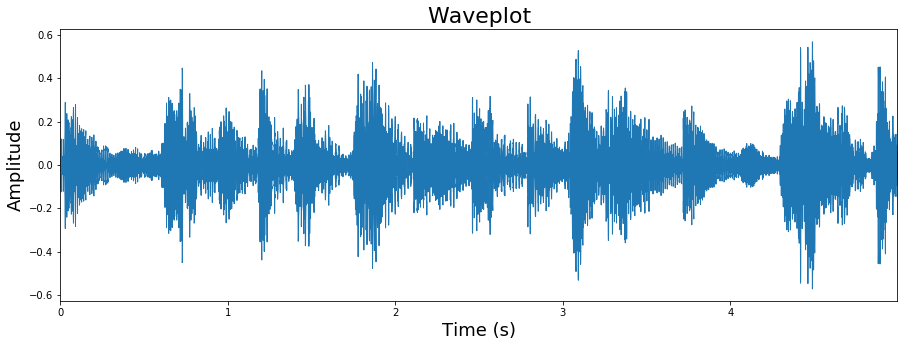
\includegraphics[scale=0.45]{img/Waveplot_Visualisation.png}
	\caption[Time-domain illustrated in wave plot]{Time-domain illustrated in wave plot}
	\label{fig:Waveplot-Time-Domain}
\end{figure}

\subsection{Frequency domain}
\label{sub:Frequency-Domain}

The frequency-domain refers to the analysis of mathematical functions or signals with respect to frequency. A frequency-domain graph shows how much of the signal lies within each given frequency band over a range of frequencies. 
\newline
\newline
A given function or signal can be converted between the time and the frequency domains with a pair of mathematical operators. The most used operation is the Fourier Transformation, which will be explained in further detail in section \ref{sub:Fourier-Transform}.

\subsection{Fourier Transform}
\label{sub:Fourier-Transform}

\gls{FT} is a mathematical concept that can convert a continuous signal from the \fullref{sub:Time-Domain} to \fullref{sub:Frequency-Domain}. It decomposes a complex periodic signal into its constituent sine waves oscillating at different frequencies, along with the magnitude of each wave. The magnitude of each frequency shows how much a certain wave contributes to the overall signal.

\subsubsection{Fast Fourier Transform}
\label{subsub:Fast-Fourier-Transform}

\gls{FFT} is a mathematical algorithm that calculates \gls{DFT} of a given sequence, with equation \ref{eq:DFT}. The only difference between \gls{FT} and \gls{FFT} is that \gls{FT} considers a continuous signal while \gls{FFT} takes a discrete signal as input. \gls{DFT} converts a sequence, a discrete signal, into its frequency constituents just like \gls{FT} does for a continuous signal. More precisely it is a transformation, which decomposes the signal into its base frequency building blocks. It is important to note that due to that transformation, the time information of the audio signal will be lost.

\myequations{Discrete Fourier Transform}
\begin{equation}
    \centering
    X_k = \sum_{n=0}^{N-1} \ x[n] \cdot e^{-\frac{i2\pi}{N}kn}
    \label{eq:DFT}
\end{equation}

\subsubsection{Short Time Fourier Transform}
\label{subsub:Short-Time-Fourier-Transform}

\gls{STFT} is a mathematical algorithm which addresses the issue, that in the \nameref{sub:Frequency-Domain} no time information exists. The \gls{STFT} calculates several \gls{FFT} at different time intervals and combines them to get information about the signal varying over time.

\subsection{Spectrogram}
\label{sub:Spectrogram}

A spectrogram is a visual representation of the \nameref{subsub:Short-Time-Fourier-Transform}. More precisely it represents the spectrum of frequencies of a signal as it varies with time. The x-axis represents the time, the y-axis represents the frequencies, and the colours represent the magnitude of the observed frequency at a particular time. Bright colours represent powerful frequencies. Thus every spectrogram represents three domains: time, frequency and magnitude.
\newline
\newline
To create a spectrogram, the audio signal is broken down into smaller frames (windows), and for each one, the \gls{DFT} or \gls{FFT} will be calculated. The resulting frequencies of each window will represent the time. It is important to note that the windows should overlap each other, not to lose any frequency. Typical window sizes are 20 to 30ms, but this size highly depends on the task to solve. Figure \ref{fig:Spectrogram} shows an example of such a spectrogram.
\begin{figure}[htbp]
	\centering
	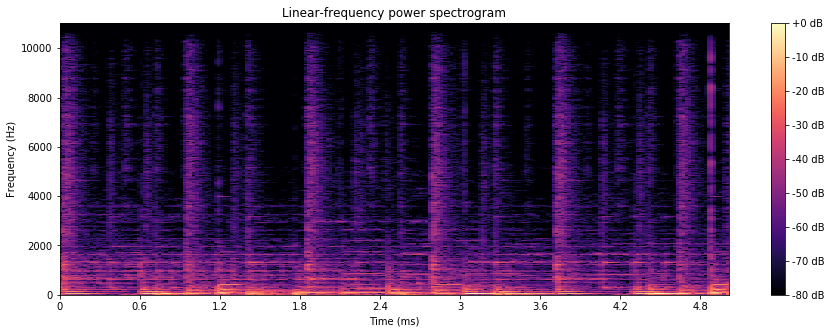
\includegraphics[scale=0.5]{img/Spectrogram_Visualisation.png}
	\caption[Example of a spectrogram]{Example of a spectrogram}
	\label{fig:Spectrogram}
\end{figure}

\subsection{Mel Spectrogram}
\label{sub:Mel-Spectrogram}

\gls{MFCC} are a feature widely used in automatic speech and speaker recognition, mainly because they focus on the audio signal and discard all other information such as background noise, emotion and many more. They were introduced by Davis and Mermelstein in the 1980s, and have been state-of-the-art ever since.
\newline
\newline
The process of creating these \gls{MFCC} are quite complex and follow five steps. Thus to the explanation of every step, there is also a short example on how to perform the step in depth. For illustration, a speech signal with a sample rate of 16kHz is assumed. The whole process is illustrated in figure \ref{fig:MFCC-Overview}.

\begin{figure}[htbp]
	\centering
    \begin{tikzpicture}[
        input/.style = {coordinate},
        output/.style = {coordinate},
        block/.style={rectangle, draw, text width=7.3em,
               text centered, rounded corners, minimum height=3em},
        arrow/.style={-{Stealth[]}}
    ]
        \node [input] (input) {};
        \node [block,right=3cm of input] (Frames)  {Break signal into overlapping frames};
        \node [block,right=of Frames] (FFT)  {Fast Fourier Transform (FFT)};
        \node [block,below right=0.2cm and 0.5cm of FFT] (MEL)  {Mel-Scale filter bank};
        \node [block,below left=0.2cm and 0.5cm of MEL] (LOG) {Log $|\cdot|$};
        \node [block,left=of LOG] (DCT) {Discrete Cosine Transform (DCT)};
        \node [output, left=3cm of DCT] (output) {};
    
        % Draw edges
        \draw [arrow] (input) -- (Frames) node [above,pos=0.25] {continuous audio} node [below,pos=0.25] {signal};
        \draw [arrow] (Frames) -- (FFT);
        \draw [arrow] (FFT)  -|  (MEL);  
        \draw [arrow] (MEL.south) |-  (LOG.east);  
        \draw [arrow] (LOG) -- (DCT) ;
        \draw [arrow] (DCT) -- node [above] {MFCC} (output);
    \end{tikzpicture}
    \caption{Steps to calculate MFCC}
    \label{fig:MFCC-Overview}
\end{figure}

\subsubsection{Frame the signal into short frames}
An audio signal is continuously changing, so to simplify it is assumed, that on short time scales the audio signal does not change much, i.e. statistically stationary. Due to that, the signal is framed into 20-40ms frames. If the frames are much shorter, there are not enough samples to get a reliable spectral estimate. If the frame length is too high, the signal changes to much throughout the frame.
\newline 
\newline
As a first step the signal has to be split into 20-40ms frames (normally 25ms is standard). The frame length for a 16kHz signal is calculated with the equation in \ref{eq:MFCC-Frame-Length}. 
\myequations{Calculate frame length from signal}
\begin{equation}
    \centering
    0.025s * 16000Hz = 400 \ \text{samples}
    \label{eq:MFCC-Frame-Length}
\end{equation}
Frame step is normally 10ms, which allows some overlap to the frames, and is calculated the same as the frame length.
\myequations{Calculate frame step from signal}
\begin{equation}
    \centering
    0.01s * 16000Hz = 160 \ \text{samples}
    \label{eq:MFCC-Frame-Step}
\end{equation}
This means that the first 400 samples start at 0, the next 400 frames start at sample 160, until the end of the speech signal is reached. If the speech signal does not divide into an even number of frames, it is padded with zeros until it does. The next steps within the example are applied to every single frame. Thus for every frame a set of features will be extracted, in this case a set of \gls{MFCC}.

\subsubsection{Calculate the periodogram estimate of the power spectrum for each frame}
The next step is to calculate the power spectrum of each frame. This is motivated by the human cochlea, an organ in the ear, which vibrates at different spots depending on the frequency of the incoming sounds. Depending on which location in the cochlea that vibrates, different nerves fire, informing the brain that specific frequencies are present. The periodogram estimate performs a similar job which is, identifying which frequencies are present in the frame.
\newline
\newline
To calculate the power spectrum for each frame, the \gls{DFT} has to be calculated with equation \ref{eq:MFCC-DFT-Frame}. Then the Periodogram-based power spectral estimate for the speech frame $s_i[n]$ can be calculated with the formula \ref{eq:MFCC-Periodogram-Frame}. Usually, a 512 point \gls{DFT} is being performed, which decomposes the signal frame $s_i[n]$ into 512 frequency building blocks and only the first 257 coefficients are kept.
\myequations{Calculate Discrete Fourier Transform of each frame}
\begin{equation}
    \centering
    S_i[k] = \sum_{n=1}^{N} s_i[n] \ h[n] \ e^{- \frac{i2\pi}{N} kn} \qquad 1 \leq k \leq K
    \label{eq:MFCC-DFT-Frame}
\end{equation}
\myequations{Calculate Periodogram-based power spectral estimate of each frame}
\begin{equation}
    \centering
    P_i[k] = \frac{1}{N}\Big|S_i[k]\Big|^2
    \label{eq:MFCC-Periodogram-Frame}
\end{equation}
where:
\begin{conditions*}
 s_i[n] &  time-domain signal frame, where $N$ denotes the frame length (in the current example from 1-400), and $i$ ranges over the number of frames \\   
 S_i[k] &  complex \gls{DFT}, where $i$ denotes the frame number corresponding to the time-domain frame \\
 h[n]   &  analysis window, with the size $N$ (e.g. hamming window) \\
 K      &  length of the \gls{DFT} \\
 P_i[k] &  power spectrum of frame $i$
\end{conditions*}

\subsubsection{Apply the Mel filterbank to the power spectra}
The periodogram spectral estimate still contains much information not required for \gls{ASR}. In the human body, the cochlea can not discern the difference between two closely spaced frequencies. This effect becomes more pronounced as the frequencies increase. For this reason, clumps of periodogram bins and sums are taken and summed up, to get an idea of how much energy exists in various frequency regions.
\newline
\newline
The Mel filterbank performs this step. The first filter of the filterbank is very narrow and indicates how much energy exists near 0 Hertz. As the frequencies get higher, the filters get wider as the variations become less relevant. The interest is only focused on how much energy occurs at each spot. The Mel scale gives the spacing and the wideness of the filterbanks. It relates perceived frequency, or pitch, of a pure tone to its actual measured frequency, it transforms the features to match more closely what humans hear. The equation \ref{eq:MFCC-Mel} converts a frequency ($f$) to the Mel scale ($m$) and equation \ref{eq:MFCC-Mel-Inv} transforms the Mels ($m$) back to a frequency ($f$).\footnote{\fullcite{anne_acoustic_2015}}
\myequations{Calculate Mel scale from frequency}
\begin{equation}
    \centering
    m = 2595 \ log_{10}(1 + \frac{f}{700Hz}) = 1127 \ log_e(1 + \frac{f}{700Hz})
    \label{eq:MFCC-Mel}
\end{equation}
\myequations{Calculate frequency from Mel scale}
\begin{equation}
    \centering
    f = 700 \ (10^{m/2595-1}) = 700 \ (e^{m/1127-1})
    \label{eq:MFCC-Mel-Inv}
\end{equation}
The Mel-spaced filterbank has to be computed to apply the filterbank to the power spectra. The filterbank is a set of 20-40 (26 is the standard) triangular filters that then are applied to the periodogram from before. The filterbank has the dimension of 26 vectors with the length 257, because in the step before the \gls{FFT} was calculated and only kept 257 coefficients. Each vector has mostly zeros in it but is non-zero for a specific section of the spectrum. Each filterbank has to be multiplied by the power spectrum. After that, the coefficients are added up to get the filterbank energies. In the end, there are 26 coefficients left, which indicates how much energy was in each filterbank. An example of a Mel-spaced filterbank is illustrated in \ref{fig:MFCC-Mel-Filterbank}.
\begin{figure}[htbp]
	\centering
	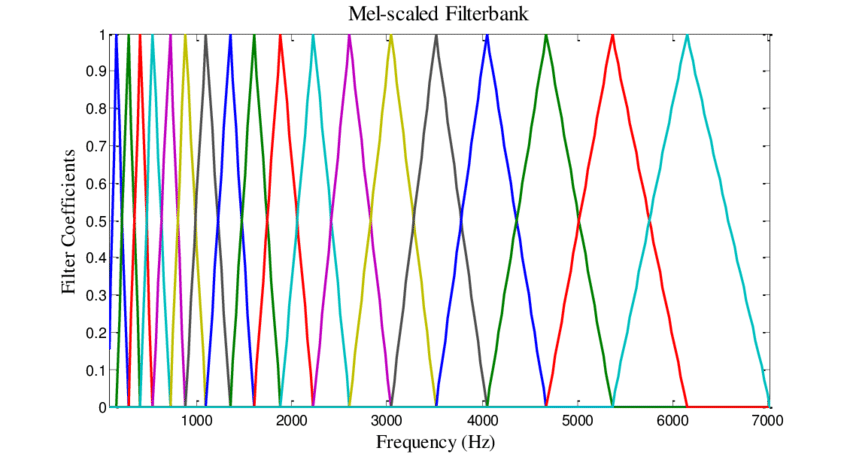
\includegraphics[scale=0.4]{img/Mel-filter-banks-basis-functions-using-20-Mel-filters-in-the-filter-bank.png}
	\caption[Mel-spaced filterbank with 20 filters]{Mel-spaced filterbank with 20 filters \footnotemark}
	\label{fig:MFCC-Mel-Filterbank}
\end{figure}
\footnotetext{\fullcite{mohd_ali_analysis_2013}}

\subsubsection{Apply the logarithm to all filterbank energies}
After the calculation of the filterbank energies, the logarithm is applied to each one of them. This operation is also inspired by human hearing because humans do not hear loudness on a linear scale. Generally to double the perceived volume of a sound eight times as much energy has to be put in. Thus if the sound signal is loud in the beginning, significant variations in energy may not sound that different. The output of this step can be visualised in a log-mel spectrogram, which is also an essential feature in audio processing.
\newline
\newline
In the above example, there are 26 energy coefficients which will be logarithmized and leaves 26 log filterbank energies.

\subsubsection{Apply the \gls{DCT} to the log filterbank energies}
The final step is to compute the \gls{DCT} of the log filterbank energies. Mainly because the filterbanks are all overlapping and are correlated with each other. The \gls{DCT} decorrelates the energies, but only the lower 12-13 of the 26 \gls{DCT} coefficients are kept. This is because the higher \gls{DCT} coefficients represent fast changes in the filterbank energies, and these fast changes can degrade the \gls{ASR} performance.
\newline
\newline
In the example, the \gls{DCT} of the 26 log filterbank energies has to be computed, which gives 26 cepstral coefficients. This whole process has to be calculated for each frame in the signal.

\subsubsection{Visualize the cepstral coefficients}
Once all the cepstral coefficients are computed, they can be visualized with respect to time. Which then can be used for further processing in \gls{ASR}. Such a visualisation is illustrated in figure \ref{fig:MFCC-Visualisation}, where the x-axis represents the time, and the y-axis represents the cepstral coefficient dimension (e.g. the lower 12-13), and the colour shows the value of each coefficient.
\begin{figure}[htbp]
	\centering
	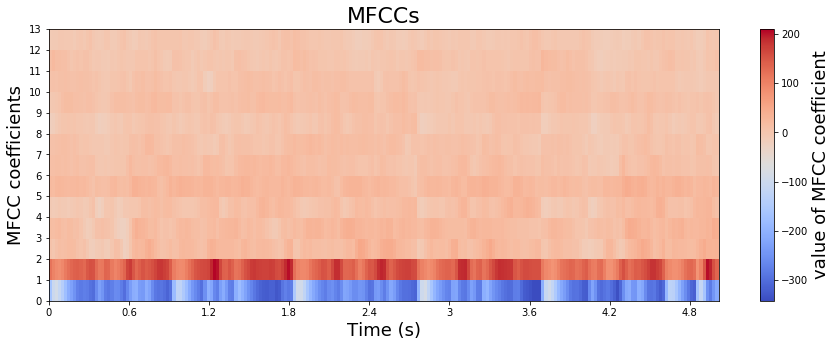
\includegraphics[scale=0.5]{img/MFCC_Visualisation.png}
	\caption[Visualisation of an MFCC]{Visualisation of a MFCC}
	\label{fig:MFCC-Visualisation}
\end{figure}

\subsection{LibROSA}
\label{sub:Librosa}

LibROSA is a python package for audio analysis and processing. At a high level, libROSA provides implementations of a variety of standard functions used throughout the field of music information retrieval. Because of this variety of realised functions, it quickly became the state-of-the-art in the field of machine learning for audio. It can easily be installed on any machine using pip.\footnote{\url{https://librosa.github.io/librosa/}}

\begin{verbatim}
    pip install librosa
\end{verbatim}

\section{Introduction to Neural Networks}
\label{sec:Intro-NN}

This section provides an introduction to an essential concept in this thesis, neural networks. They will be used to build the model and tackle the problem. First, a general \fullref{sub:Neural-Network} is introduced to clarify some terminology. After that, \fullref{sub:Convolutional-Neural-Network} and \fullref{sub:Gated-Recurrent-Unit} will be explained to give an overview of some specialized kind of neural networks.

\subsection{Neural Network}
\label{sub:Neural-Network}


\begin{figure}[htbp]
    \centering
    \begin{tikzpicture}
    
    \def\nodedist{45pt}
    \def\layerdist{70pt}
    \def\pindist{20pt}
    
    \tikzstyle{every pin edge}=[signal]
    \tikzstyle{annot} = [text width=4em, text centered]
    
    % input nodes
    \foreach \y in {1,...,3}
        \node[inputnode, pin={[pin edge={latex-}, pin distance=\pindist]left:Input \y}] 
            (x\y) at (0,-\y*\nodedist) {$x_\y$};
    
    % sum
    \node[infonode] 
            (sigma) at ($(x2) + (\layerdist, -0*\nodedist)$) {$\displaystyle\Sigma$};
            
    % bias
    \node[inputnode, label=above:{\parbox{2cm}{\centering Bias}}] at (sigma|-x1) (b1) {$b_1$};
    
    % activation function
    \node[infonode, label=above:{\parbox{2cm}{\centering Activation\\ function}}] 
            (activation) at ($(sigma) + (\layerdist, -0*\nodedist)$) {$f(z)$};
            
    % output node
    \node[outputnode, pin={[pin edge={-latex}, pin distance=\pindist]right:Output}]
            (output) at ($(activation) + (\layerdist, -0*\nodedist)$) {$\hat{y}$};
    
    % arrows 
    \draw[signal] (x1) -- (sigma) node [below right=0.25 and 0.05 of x1] {$\theta_{1}$};
    \draw[signal] (x2) -- (sigma) node [below right=-0.1 and 0.05 of x2] {$\theta_{2}$};
    \draw[signal] (x3) -- (sigma) node [below right=-0.5 and 0.05 of x3] {$\theta_{3}$};
    \draw[signal] (b1) -- (sigma);
    \draw[signal] (sigma) -- (activation);
    \draw[signal] (activation) -- (output);
    
    \end{tikzpicture}
    \caption{Visualization of a perceptron}
    \label{fig:Perceptron-Visualisation}
\end{figure}
\noindent
Warren McCulloch and Walter Pitts introduced the first \gls{NN} in 1943 within the paper (\cite{mcculloch_logical_1943}), where they proposed a computational model for a \gls{NN} based on algorithms called threshold logic. To develop the \gls{NN}, they used observations about the neurophysiology of the brain. In simplified terms, the brain can be described similar to a net of neurons where each neuron has a soma and an axon. The soma denotes the corpus of the neuron and the axon a nerve’s extension for the connection with others. Synapses exist between the axon of one neuron and the soma of another. The neuron sends an impulse if its excitation exceeds a certain threshold. Later in 1958 Frank Rosenblatt extended this idea of a \gls{NN} to the Perceptron formulation (\cite{rosenblatt_perceptron_1958}). It is one of many neuron representations which have been used within neural networks so far.
\newline
\newline
A perceptron is the simplest neural network which consists of $n$ number of inputs and only one output. It further consists of multiple inputs, weights, a bias, an activation function and an output. The building blocks and the procedure of calculating an output are visualised in figure \ref{fig:Perceptron-Visualisation}.

\begin{figure}[htbp]
    \centering
    \subfloat[Sigmoid]{
            \begin{tikzpicture}
            \begin{axis}[legend pos=north west, width=5cm,height=4.5cm,ylabel=$\sigma(z)$,xlabel=$z$,ymin=0,ymax=1.25,xmin=-5,xmax=5]
                \addplot[blue,smooth] {1/(1+exp(-x))};
                \addlegendentry{$\frac{1}{1+e^{-z}}$}
            \end{axis}
        \end{tikzpicture}
    }
    \subfloat[Tanh]{
        \begin{tikzpicture}
            \begin{axis}[legend pos=north west, width=5cm,height=4.5cm,ylabel=$\tanh(z)$,xlabel=$z$,ymin=-1.25,ymax=1.25,xmin=-5,xmax=5]
                \addplot[blue,smooth] {tanh(x)};
                \addlegendentry{$\frac{2}{1+e^{-2x}} -1$}
            \end{axis}
        \end{tikzpicture}
    }
    \subfloat[ReLU]{
            \begin{tikzpicture}
            \begin{axis}[legend pos=north west, width=5cm,height=4.5cm,ylabel=$s(z)$,xlabel=$z$,ymin=-0.5,ymax=1.25,xmin=-2.5,xmax=2.5]
                \addplot[samples=500, blue] {max(0, x)};
                \addlegendentry{$max(0, z)$}
            \end{axis}
        \end{tikzpicture}
    }
    \caption{Graphical representation of non-linear activation functions}
    \label{fig:Activation-Functions}
\end{figure}
\noindent
The inputs which are denoted as $x_1, \dots, x_n$, are the values passed into the perceptron. The weights $\theta_{1}, \dots, \theta_{n}$ are values which are multiplied with the respective input, the bias is a special weight which shifts the activation function to the left or right. And the activation function $f(z)$ is used to introduce non-linearity into the output. Without the \gls{NN} would represent a linear function. With the non-linearity of the activation function, a layered \gls{NN} with enough capacity can learn any function. Such non-linear activation functions are illustrated in figure \ref{fig:Activation-Functions}. The output $\hat{y}$ is simply the result of the activation function, and it can be computed using equation \ref{eq:Perceptron-Calculate-Output}. In the case of a perceptron, it is the output of the \gls{NN}. The process of calculating the output of a \gls{NN} is called forward propagation.
\myequations{Calculates the output of single layer neural network}
\begin{equation}
    \centering
    \hat{y} = f(z) = f\Big(b_1 + \sum_{i=1}^n x_i \theta_i \Big)
    \label{eq:Perceptron-Calculate-Output}
\end{equation}
In deeper networks, the output of one layer is then used again as the input of the next layer $f^L(f^{L-1}(\cdots f^1(z)))$, where $L$ denotes the number of layers in the \gls{NN}. A layer consists of multiple perceptrons. Thus this is often called a \gls{MLP}, which is illustrated in figure \ref{fig:MLP-Visualisation}. $z_1^1$ is one example of a single perceptron within the network. The \gls{MLP} shown in figure \ref{fig:MLP-Visualisation} has four layers ($L = 4$), from which the first one is always the input layer, and the last one is the output layer. The layers between the input and output layer are called hidden layers. These layers are also called fully connected layers, because there is a corresponding weight to each input of the next layer.

\begin{figure}[htbp]
    \centering
    \begin{tikzpicture}[]
        \def\nodedist{35pt}
        \def\layerdist{80pt}
        \def\pindist{20pt}
        
        \tikzstyle{every pin edge}=[signal]
        \tikzstyle{annot} = [text width=4em, text centered]
        
        \foreach \y in {1,...,3}
            \node[inputnode, pin={[pin edge={latex-}, pin distance=\pindist]left:Input \y}] 
                (I\y) at (0,-\y*\nodedist) {$x_\y$};  
    
        \foreach \y in {1,...,4}
            \node[hiddennode] 
                (H1\y) at ($(\layerdist,-\y*\nodedist) +(0, 0.5*\nodedist)$) {$z_\y^1$};
        
        \foreach \y in {1,...,4}
            \node[hiddennode] 
                (H2\y) at ($(2*\layerdist,-\y*\nodedist) +(0, 0.5*\nodedist)$) {$z_\y^2$};
        
        \foreach \y in {1,...,2}
            \node[outputnode, pin={[pin edge={-latex}, pin distance=\pindist]right:Output \y}]
                (O\y) at ($(H21) + (\layerdist, -\y*\nodedist)$) {$\hat{y}_\y$};
    
        \foreach \dest in {1,...,4}
            \foreach \source in {1,...,3}
                \draw[signal] (I\source) -- (H1\dest);
        
        \foreach \dest in {1,...,4}
            \foreach \source in {1,...,4}
                \draw[signal] (H1\source) -- (H2\dest);
        
        \foreach \dest in {1,...,2}
            \foreach \source in {1,...,4}
                \draw[signal] (H2\source) edge (O\dest);
    
        \node[annot, above=4pt of H11] (hl) {Hidden layer 1};
        \node[annot, above=4pt of H21] (hl) {Hidden layer 2};
        \node[annot] at (I1 |- hl) {Input layer};
        \node[annot] at (O1 |- hl) {Output layer};
    \end{tikzpicture}
    \caption{Visualization of a multilevel perceptron}
    \label{fig:MLP-Visualisation}
\end{figure}
\noindent
In order that the \gls{NN} produces more reliable results, it has to learn the optimal parameters for a given problem. This procedure consists of two parts, backpropagation and optimisation. Backpropagation refers to the algorithm for computing the gradient of the loss function with respect to the parameters, to see how good the current predictions are. However, the term is often used to refer to the entire learning algorithm, including optimization. Furthermore, optimisation is the process of selecting the best element from some set of available alternatives, which in the case of a \gls{NN} is the selection of the best parameters.
\newline
\newline
The first step in backpropagation is to know an estimation of how far away the current predictions are from the desired solution, which can be computed using a loss function. Typical loss functions are \gls{MSE}, Binary Crossentropy, Categorical Crossentropy or Sparse Categorical Crossentropy. The process of selecting the right loss function highly depends on the problem to solve. The equation \ref{eq:MSE} defines the \gls{MSE} cost (loss) function $\mathcal{L}$ for the entire dataset with size $n$.
\myequations{Mean Squared Error loss function for entire dataset}
\begin{equation}
    \centering
    \mathcal{L} = MSE = \frac{1}{n} \sum_{i=1}^n(y_i - \hat{y}_i)^2
    \label{eq:MSE}
\end{equation}
where:
\begin{conditions*}
    y_i & actual value from the dataset \\   
    \hat{y}_i & predicted value, output of the \gls{NN}
\end{conditions*}
\noindent
The next step in backpropagation is to calculate the error of each weight $\theta_i$. The bias $b_i$ can also be thought of as a special kind of weight within the network. This is done by computing the gradients, given the cost function $\mathcal{L}$, with respect to the weights $\theta_i$. The gradient can be interpreted as the direction and rate of fastest increase. 
\newline
\newline
In equation \ref{eq:Backpropagation-Gradient} the gradient of the cost function $\mathcal{L}$ with respect to the weights $\theta_i$ is computed using partial derivation. The equation computes the gradients of the weights from the last hidden layer (\flqq Hidden layer 2\frqq, e.g. $z^2_1$) shown in figure \ref{fig:MLP-Visualisation}. For lower layers, the chain rule would be used more extensively. The same function can also be used to compute the cost function $\mathcal{L}$ with respect to the bias. Since the cost function is not directly related to the weights, the chain rule is used.
\myequations{Gradient of cost function with respect to the weights}
\begin{equation}
    \centering
    \frac{\partial \mathcal{L}}{\partial\theta_i} = \frac{\partial \mathcal{L}}{\partial\hat{y}}\times\frac{\partial\hat{y}}{\partial z}\times\frac{\partial z}{\partial\theta_i}
    \label{eq:Backpropagation-Gradient}
\end{equation}
The last step in the learning process of a \gls{NN} is the optimisation. Gradient descent is one of many optimisation algorithms, and it changes the weights and bias, proportional to the negative of the gradient of the cost function with respect to the corresponding weight or bias. Learning rate $\alpha$ is a hyperparameter, which is used to control how much the weights and bias change. The weights and bias are updated with equations \ref{eq:Optimisation-Gradient-Descent-Weights}.
\myequations{Optimisation of weights using gradient descent}
\begin{equation}
    \centering
    \theta_i = \theta_i - \Big(\alpha \times \frac{\partial \mathcal{L}}{\partial\theta_i}\Big)
    \label{eq:Optimisation-Gradient-Descent-Weights}
\end{equation}
The whole learning process consisting of backpropagation and optimisation is repeated until the \gls{NN} convergences in a local or global minimum.
\newline
\newline
\gls{MLP} have several drawbacks, especially when it comes to handling two-dimensional data, for example, audio or image data. \gls{MLP} use one perceptron for each input (e.g. pixel in an image, multiplied by 3 in the case of RGB). The amount of weights rapidly becomes unmanageable for large input data. In case of a 224 x 224 pixel image with three colour channels, there are around 150'000 weights that must be trained. As a result, difficulties arise while training and overfitting can occur. Another common problem is that \gls{MLP} react differently to an input and its shifted version — they are not translation invariant. For example, if a picture of a cat appears in the top left of the image in one picture and the bottom right of another picture, the \gls{MLP} will try to correct itself and assume that a cat will always appear in this section of the image. All the problems stated above also apply to other areas. Thus \gls{MLP} are not the best idea to use for two-dimensional data. In the next section, \fullref{sub:Convolutional-Neural-Network} will be introduced, which will solve the problems stated above.

\subsection{Convolutional Neural Network}
\label{sub:Convolutional-Neural-Network}

\gls{CNN} are a specialized kind of neural network for processing data that has a known grid-like topology. Examples include time-series data, which can be thought of as a 1-D grid taking samples at regular time intervals, and image data, which can be thought of as a 2-D grid of pixels. The name \flqq convolutional neural network\frqq \ indicates that the network employs a mathematical operation called convolution. Convolution is a specialized kind of linear operation. To summarize, a \gls{CNN} are simply neural networks that use convolution in place of general matrix multiplication in at least one of their layers.\footnote{\fullcite{goodfellow_deep_2016}}
\newline
\newline
A typical layer of a \gls{CNN} consists of three stages, which is illustrated in figure \ref{fig:Convolution-Layer-Visualisation}. In the first stage, the layer performs several convolutions in parallel to produce a set of linear activations, also called a feature map. In the second stage, each linear activation is run through a non-linear activation function, such as the rectified linear activation function. This stage is sometimes called the detector stage. In the third stage, a pooling function is used to modify the output of the layer further.

\begin{figure}[htbp]
    \captionsetup{format=plain}
    \centering
    \begin{tikzpicture}[start chain=going below, node distance=15pt,
        point/.append style={on chain, join=by {signal}},
        layer/.append style={on chain, join=by {signal}},
    ]
        \node[point] {Input to layers};
        \node[conv] {Convolution layer: \\ affine transform};
        \node[activation] {Detector layer: \\ non-linearity (e.g., ReLU)};
        \node[pool] {Pooling layer};
        \node[point] {Next layer};
    \end{tikzpicture}
    \caption{Visualisation of a single convolutional layer}
    \label{fig:Convolution-Layer-Visualisation}
\end{figure}
\noindent
Convolution is a process where a small matrix of numbers, called the kernel or filter, is taken and slid it over grid-like data (e.g. an image) and transforms it based on the values from the filter. More concretely, at a given position of the convolution kernel, the element-wise multiplication of each kernel cell value and the corresponding image pixel value that overlaps the kernel cell is taken and then summed up. The convolutional operation is often denoted as $\ast$, the equation \ref{eq:Convolution} shows how to calculate the convolution of an input image $I$ and a two-dimensional filter kernel $K$ with the filter size $(m, n)$. The rows and the columns of the input image $I$ are denoted as $i$ and $j$. The output of the convolutional operation $S(i,j)$ is often called the feature map. A visualisation of the operation is illustrated in figure \ref{fig:Convolution-Visualisation}. In the context of \gls{CNN}, the learning algorithm will learn the appropriate values of the kernel in the appropriate place, to detect arbitrary features.
\myequations{Convolution of an image and a two-dimensional kernel}
\begin{equation}
    \centering
    S(i,j) = (K \ast I)(i,j) = \sum_{m=-\infty}^\infty \sum_{n=-\infty}^\infty I(i-m, j-n) \cdot K(m,n)
    \label{eq:Convolution}
\end{equation}
The goal of the convolutional operation in the \gls{CNN} is to output a high value for a given position, if the kernel is present in that location, else outputs a low value. The convolutions are restricted to only \flqq valid\frqq \ positions, where the kernel lies entirely within the image. Since the image shrinks every time a convolution is performed, it can only be performed a limited number of times. Furthermore, it can be seen that the kernel has a more significant impact on the centre of the image as on the outskirts. The image will be padded with an additional border, to solve both of these problems. Usually, it is filled with zeros. Depending on whether padding is used or not, there are two types of convolution: Valid and Same. Valid means that the original image is used and same states, that padding around the image is used and thus the input and output image have the same size. Another important hyperparameter of a \gls{CNN} is stride, which indicates how much the kernel slides to its next position. Figure \ref{fig:Convolution-Visualisation} illustrates a convolution with a 2x2 kernel, padding valid and stride one. 

\begin{figure}[htbp]
    \captionsetup{format=plain}
    \centering
    \begin{tikzpicture}
        \coordinate (p) at (0,0);
        \draw[shift={(p)}, fill=white] (0,0) rectangle (4,-3);
        \draw[shift={(p)}, fill=blue!20!white] (0,0) rectangle (2,-2);
        \draw[
            ultra thick,
            step=1, 
            color=black,
            draw=black,
            fill=black!20!white,
            shift={(p)}
        ] (0,0) grid (4,-3)
        foreach[count=~] \l in {9, 0, 3, 8, 1, 2, 4, 3, 6, 4, 0, l} {
            ({0.5+mod(~-1,4}, {-0.5-div(~-1,4}) node {\Large \l}
        };
        
        \node[text width=1cm] at (5,-1.5) {$\Large\ast$};
        
        \coordinate (p) at (5.2,-0.5);
        \draw[shift={(p)}, fill=blue!20!white] (0,0) rectangle (2,-2);
        \draw[
            ultra thick,
            step=1, 
            color=black,
            draw=black,
            fill=black!20!white,
            shift={(p)}
        ] (0,0) grid (2,-2)
        foreach[count=~] \l in {1, 2, -1, -2} {
            ({0.5+mod(~-1,2}, {-0.5-div(~-1,2}) node {\Large \l}
        };
        
        \node[text width=1cm] at (8.2,-1.5) {$\Large =$};
        
        \coordinate (p) at (8.5,-0.5);
        \draw[shift={(p)}, fill=white] (0,0) rectangle (3,-2);
        \draw[shift={(p)}, fill=blue!20!white] (0,0) rectangle (1,-1);
        \draw[
            ultra thick,
            step=1, 
            color=black,
            draw=black,
            fill=black!20!white,
            shift={(p)}
        ] (0,0) grid (3,-2)
        foreach[count=~] \l in {4, -4, 9, -9, 6, -8} {
            ({0.5+mod(~-1,3}, {-0.5-div(~-1,3}) node {\Large \l}
        };
    \end{tikzpicture}
    \caption[Visualization of a convolutional operation]{Visualization of a convolutional operation. To calculate the value highlighted in blue within the feature map (right), the equation \ref{eq:Convolution} has to be used. Thus the highlighted element can be calculated with $9\cdot 1 + 0\cdot 2 + 1\cdot (-1) + 2\cdot (-2) = 4$}
    \label{fig:Convolution-Visualisation}
\end{figure}
\noindent
A pooling function replaces the output of the net at a particular location with a summary statistic of the nearby outputs. For example, the max-pooling operation reports the maximum output within a rectangular neighbourhood. Another popular pooling function is the average-pooling, which outputs the average number within a rectangular neighbourhood. Both pooling functions are illustrated in figure \ref{fig:Pooling-Visualisation}. Pooling helps to make the representation approximately invariant to small translations of the input. Invariance to translation means that if a small amount translates the input data, the values of most of the pooled outputs do not change. Invariance to local translation can be a useful property if the focus is more on whether some feature is present within the data than exactly where it is located.

\begin{figure}[htbp]
    \centering
    \begin{tikzpicture}
        \coordinate (p) at (0,0);
        \draw[shift={(p)}, fill=red!20!white] (0,0) rectangle (2,-2);
        \draw[shift={(p)}, fill=yellow!20!white] (2,0) rectangle (4,-2);
        \draw[shift={(p)}, fill=blue!20!white] (0,-2) rectangle (2,-4);
        \draw[shift={(p)}, fill=green!20!white] (2,-2) rectangle (4,-4);
        \draw[
            ultra thick,
            step=1, 
            color=black,
            draw=black,
            fill=black!20!white,
            shift={(p)}
        ] (0,0) grid (4,-4)
        foreach[count=~] \l in {73, 74, 17, 49, 10, 29, 41, 20, 4, 23, 39, 4, 50, 80, 56, 57} {
            ({0.5+mod(~-1,4}, {-0.5-div(~-1,4}) node {\Large \l}
        };
        
        % max pooling
        \coordinate (p) at (7,0.5);
        \draw[shift={(p)}, fill=red!20!white] (0,0) rectangle (1,-1);
        \draw[shift={(p)}, fill=yellow!20!white] (1,0) rectangle (2,-1);
        \draw[shift={(p)}, fill=blue!20!white] (0,-1) rectangle (1,-2);
        \draw[shift={(p)}, fill=green!20!white] (1,-1) rectangle (2,-2);
        \draw[
            ultra thick,
            step=1, 
            color=black,
            draw=black,
            fill=black!20!white,
            shift={(p)}
        ] (0,0) grid (2,-2)
        foreach[count=~] \l in {74, 49, 80, 57} {
            ({0.5+mod(~-1,2}, {-0.5-div(~-1,2}) node {\Large \l}
        };
        \draw[signal] (4.5,-1.5) -> ($(p) +(-0.5, -1.25)$);
        \node[text width=100pt, align=center, right of=p, yshift=10pt] (l1) {Max-Pooling};
        
        % average pooling
        \coordinate (p) at (7,-2.5);
        \draw[shift={(p)}, fill=red!20!white] (0,0) rectangle (1,-1);
        \draw[shift={(p)}, fill=yellow!20!white] (1,0) rectangle (2,-1);
        \draw[shift={(p)}, fill=blue!20!white] (0,-1) rectangle (1,-2);
        \draw[shift={(p)}, fill=green!20!white] (1,-1) rectangle (2,-2);
        \draw[
            ultra thick,
            step=1, 
            color=black,
            draw=black,
            fill=black!20!white,
            shift={(p)}
        ] (0,0) grid (2,-2)
        foreach[count=~] \l in {46, 32, 39, 39} {
            ({0.5+mod(~-1,2}, {-0.5-div(~-1,2}) node {\Large \l}
        };
        \draw[signal] (4.5,-2.5) -> ($(p) +(-0.5, -0.75)$);
        \node[text width=100pt, align=center, right of=p, yshift=10pt] (l1) {Average-Pooling};
    \end{tikzpicture}
    \caption{Visualisation of the max- and average-pooling operation}
    \label{fig:Pooling-Visualisation}
\end{figure}
\noindent
Almost every \gls{CNN} has some fully connected layers in the last layer because they will combine the features learnt by different convolution kernels so that the network can build a global representation about the holistic input data. The neurons in the fully connected layer will get activated based on whether various entries, represented by convolution features, are present in the inputs. This provides a compact representation of features existing in the input to the output layer, which the output layer can easily use to classify the input data correctly.
\newline
\newline
To create a \gls{CNN}, all of the above concepts have to be put together to form an end-to-end model, from a raw input data to a decision. To summarise, the convolution layers will learn various local features in the data (e.g. what an eye looks like), then the pooling layer will make the \gls{CNN} invariant to translations of these features (e.g. if the eye appears slightly translated in two images, the \gls{CNN} will still recognise it as an eye). Finally, the fully connected layers combine the found features and activate the correct output (e.g. there are two eyes, a nose and a mouth, this must be a person).

\subsubsection{Dilated Convolution}
\label{subsub:Dilated-Convolution}

Dilated convolution is a specialized type of convolution, which was first introduced within the paper (\cite{yu_multi-scale_2016}). It is helpful first to understand why vanilla convolutions (normal convolutions) struggle to integrate the global context. Suppose a purely convolutional network composed of layers of $k \times k$ convolutions, without pooling. It is clear to see that size of the receptive field of each unit (the block of pixels which can influence its activation) is $l \times (k-1) + k$, where $l$ is the layer index. Therefore the effective receptive field of units can only grow-linearly with the layers. Especially for high-resolution input images, the linearly-grow is very limiting.
\newline
\newline
Dilated convolutions increase the kernel by inserting spaces between the kernel elements. The dilation rate is controlled by an additional hyperparameter $l$. These one dimensional dilated convolutions between signal $I$ and kernel $K$ and dilation factor $l$ is defined by formula \ref{eq:Dilated-Convolution}. $\ast_l$ refers to the dilated convolution or a $l$-dilated convolution. The normal convolution $\ast$ is simply the 1-dilated-convolution. The figure \ref{fig:Dilated-Convolution} illustrates stacked dilated convolutions within a \gls{CNN}, where the dilation factor $l$ is increased exponentially.
\myequations{Convolution of an image and a two-dimensional kernel}
\begin{equation}
    \centering
    (K \ast_l I)(i) = \sum_{n=-\infty}^\infty K(n) \cdot I(i - ln)
    \label{eq:Dilated-Convolution}
\end{equation}
Dilated convolutions are used to cheaply increase the receptive field of output units without increasing the kernel size, which is especially useful when multiple dilated convolutions are stacked one after another. For a concrete example, see \cite{oord_wavenet_2016}, in which the proposed WaveNet model implements an autoregressive generative model for raw audio which uses dilated convolutions to condition new audio frames on a broad context of past audio frames.

\begin{figure}[htbp]
	\centering
	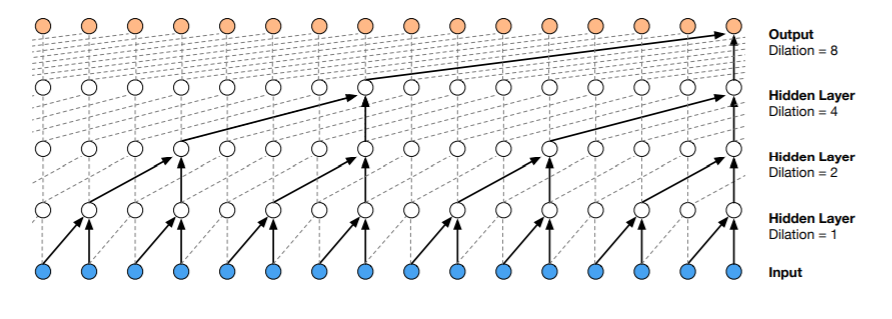
\includegraphics[scale=0.9]{img/Dilated_Colvolution.png}
	\caption[SINS database recording environment map]{Visualisation of stacked diluted convolutions \footnotemark}
	\label{fig:Dilated-Convolution}
\end{figure}
\footnotetext{\fullcite{oord_wavenet_2016}}

\subsection{Gated Recurrent Unit}
\label{sub:Gated-Recurrent-Unit}

\gls{GRU} are a specialised type of \gls{NN} within the family of \gls{RNN}, which focus on processing sequential data. \gls{GRU} were introduced in the paper (\cite{cho_learning_2014}) to solve the vanishing gradient problem, which comes with a standard \gls{RNN}. \gls{RNN} take as their input, not just the current input example they see, but also what they have perceived previously. It can be thought of multiple feed-forward neural networks, passing information from one to the other. The vanishing gradient problem states that input from far behind (e.g. the first sample in a sequence) loses its importance in the last inputs (e.g. the last sample of a sequence), because it vanishes along the way.

\begin{figure}[htbp]
    \captionsetup{format=plain}
    \centering
    \begin{tikzpicture}[thick, node distance=30pt and 30pt, on grid]
        \node[cell, minimum width=200pt, minimum height=110pt, anchor=north west] (b) at (-2pt,0pt) {};
        
        \coordinate (hin) at (0pt,-20pt);
        \draw[signal] (hin) +(-\iolen, 0pt) node[above] {$h_{t-1}$} -- (hin);
        \coordinate (hout) at (200pt,-20pt);
        \draw[signal] (hout) -- +(\iolen,0pt) node[above left] {$h_{t}$};
        \coordinate (h) at (184pt,0pt);
        \draw[signal] (h) -- +(0,\iolen) node[left] {$h_{t}$};
        \coordinate (x) at (14pt,-110pt);
        \draw[signal, -] (x) +(0pt,-\iolen) node[left] {$x_{t}$} -- (x);
        
        \node[celllayer] (r) at (68pt,-80pt) {$\sigm$};
        \node[celllayer, right=58pt of r] (z) {$\sigm$};
        \node[celllayer, right=34pt of z] (ht) {$\tanh$};
        
        \node[pointwise, above=30pt of ht] (htm) {$\times$};
        \draw[signal] (ht) edge node[pos=0.5,left] {$\tilde{h}_t$} (htm);
        \node[pointwise, above=30pt of htm] (htmp) {$+$};
        \draw[signal] (htm) -- (htmp);
        \draw[signal, -] (htmp) -- (hout);
        
        \node[pointwise, above left=30pt and 30pt of z] (z1) {$-1$};
        \draw[signal] (z) |- (z1) node[pos=0.2,left] {$z_t$};
        \node[pointwise, above=30pt of z1] (z1m) {$\times$};
        \draw[signal] (z1) -- (z1m);
        \draw[signal, -] (z1m) -- (htmp);
        \draw[signal] (z) |- (htm);
        \draw[signal, -] (hout -| h) +(-10pt,0pt) -| (h);
        
        \draw[signal, -] (hin) +(-10pt,0pt) -- (z1m);
        
        \node[pointwise, above left=30pt and 30pt of r] (rm) {$\times$};
        \draw[signal] (r) |- (rm) node[pos=0.2,left] {$r_t$};
        \draw[signal] (hin -| rm) +(-10pt,0pt) -| (rm);
        
        \coordinate (hx) at (60pt,-94pt);
        \draw[signal, -] (x) |- (hx);
        \draw[signal, -] (hin) +(-10pt,0pt) -| (x |- r) |- (hx) +(10pt,0pt);
        \draw[signal, -] (hx) -| (r);
        \draw[signal, -] (hx) -| (z);
        
        \coordinate (rx) at (60pt,-102pt);
        \draw[signal, -] (x) |- (rx);
        \draw[signal, -] (rx) -| (ht);
        
        \draw[signal, -, shorten >=\intergape] (rm) |- (rm |- hx);
        \draw[signal, -, shorten <=\intergape] (rm |- hx) |- (z |- rx);
    \end{tikzpicture}
    % legend
    \begin{tikzpicture}
    	\def\labeldist{30pt}
    	\def\nodedist{60pt}
    
    	\node[celllayer, minimum width=40pt] (l) at (0pt,0pt) {};
    	\node[align=center] at ($(l) +(0pt,-\labeldist)$) {Network\\Layer}; % trainable
    	\node[pointwise] (p) at ($(l) +(\nodedist, 0pt)$) {};
    	\node[align=center] at ($(p) +(0pt,-\labeldist)$) {Pointwise\\Operation};
    	\coordinate (v) at ($(p) +(\nodedist, 0pt)$);
    	\draw[signal] (v) +(-20pt,0pt) -- +(20pt, 0pt);
    	\node[align=center] at ($(v) +(0pt,-\labeldist)$) {Vector\\Transfer};
    	\coordinate (m) at ($(v) +(\nodedist, 0pt)$);
    	\draw[signal] (m) +(-10pt,10pt) |- +(10pt, 0pt);
    	\draw[signal] (m) +(-10pt,-10pt) |- +(10pt, 0pt);
    	\node[align=center] at ($(m) +(0pt,-\labeldist)$) {Concatenate};
    	\coordinate (c) at ($(m) +(\nodedist, 0pt)$);
    	\draw[signal] (c) +(-10pt,0pt) -| +(10pt, 12pt);
    	\draw[signal] (c) +(-10pt,0pt) -| +(10pt, -12pt);
    	\node[align=center] at ($(c) +(0pt,-\labeldist)$) {Copy};
    \end{tikzpicture}
    \caption[Visualisation of a single gated recurrent unit]{Visualisation of a single gated recurrent unit. In the illustration, the Hadamard product $\odot$ is denoted as $\times$.}
    \label{fig:GRU-Visualisation}
\end{figure}
\noindent
\gls{GRU} is an improved version of the standard \gls{RNN}, which use an update- and reset gate to solve the vanishing gradient problem. These gates are two additional vectors which decide what information should be passed to the output. They can be trained to keep information from long ago, without washing it through time or remove information which is irrelevant to the prediction. Figure \ref{fig:GRU-Visualisation} illustrates a single \gls{GRU} cell, which will be used to get a better understanding of how the \gls{GRU} works. The Hadamard product $\odot$ is also known as an element-wise multiplication.
\newline
\newline
The update gate is denoted as $z_t$ and will be calculated for time step $t$ with the equation in \ref{eq:GRU-Update-Gate}. When $x_t$ is fed into the network unit, it is multiplied by its own weight $W^{(z)}$. The same will be done to $h_{t-1}$, which denotes the information from the previous $t-1$ units and is multiplied by its own weight $U^{(z)}$. Both results are added together, and a sigmoid activation function is applied to squash the result between 0 and 1. The update gate helps the model to determine how much of the past information needs to be passed along to the future. This eliminates the vanishing gradient problem because the model can decide to copy all the information from the past without losing any data.
\myequations{Gated recurrent unit update gate}
\begin{equation}
    \centering
    z_t = \sigma(W^{(z)}x_t + U^{(z)}h_{t-1})
    \label{eq:GRU-Update-Gate}
\end{equation}
$r_t$ denotes the reset gate, which is used to decide how much of the past information the model has to forget, it is defined by the equation \ref{eq:GRU-Forget-Gate}. The formula is the same as the one used to calculate the update gate \ref{eq:GRU-Update-Gate}. The difference appears in the weights and the usage of the gate.
\myequations{Gated recurrent unit forget gate}
\begin{equation}
    \centering
    r_t = \sigma(W^{(z)}x_t + U^{(z)}h_{t-1})
    \label{eq:GRU-Forget-Gate}
\end{equation}
$\tilde{h}_t$ is called a memory content, which uses the reset gate to store the relevant information from the past. It is calculated using equation \ref{eq:GRU-Memory-Content}. Calculating the Hadamard product between the reset gate $r_t$ and $Uh_{t-1}$ will determine what to remove from the previous time steps.
\myequations{Gated recurrent unit memory content}
\begin{equation}
    \centering
    \tilde{h}_t = tanh(Wx_t + r_t \odot Uh_{t-1})
    \label{eq:GRU-Memory-Content}
\end{equation}
The last step within the network unit is to calculate $h_t$, which holds information for the current unit and passes it down to the network. The update gate is needed within this step to determine what to collect from the current memory content $\tilde{h_t}$, as well as to decide what to collect from the previous steps $h_{t-1}$. The equation to calculate $h_t$ is shown in \ref{eq:GRU-Output}.
\myequations{Gated recurrent unit output}
\begin{equation}
    \centering
    h_t = z_t \odot h_{t-1} + (1-z_t) \odot \tilde{h}_t
    \label{eq:GRU-Output}
\end{equation}
\gls{GRU} can store and filter the information using their update and reset gates. These gates eliminate the vanishing gradient problem since the model is not washing out the new input every single time, but keeps the relevant information and passes it down to the next time steps of the network. \gls{GRU} can perform exceptionally well, even in very complex environments.

\subsection{Tensorflow}
\label{sub:Tensorflow}

TensorFlow is an end-to-end open-source platform for machine learning. It has a comprehensive, flexible ecosystem of tools, libraries and community resources that lets researchers push the state-of-the-art in \gls{ML} and developers easily build and deploy \gls{ML} powered applications.\footnote{\url{https://www.tensorflow.org/}}

\begin{verbatim}
    # Release for CPU-only
    pip install tensorflow==2.1
    
    # Release with GPU support (Ubuntu and Windows)
    pip install tensorflow-gpu==2.1 
\end{verbatim}

\section{Introduction to Clustering}
\label{sec:Intro-Clustering}

Clustering is considered to be one of the essential techniques of unsupervised learning and can be used in various applications, such as spam filtering, identifying fake news and segmentation of costumers. 
\newline
\newline
It is the process of dividing the entire dataset into groups, also known as clusters, based on the patterns in the data. It also finds hidden relationships between data points and gives valuable insights into the dataset. A cluster is the collection of data objects which are similar to one another within the same group and are different from the objects in other clusters.
\newline
\newline
Clustering is not part of the scope of the thesis and will, therefore, only be used to visualise and evaluate the embeddings produced by the network.

\subsection{K-Means}
\label{sub:K-Means}

K-Means clustering is one of the most straightforward yet powerful unsupervised machine learning algorithms. The objective of the clustering algorithm is to group similar data points and discover underlying patterns. To achieve this objective, K-means looks for a fixed number of clusters $k$ in a dataset. The number of clusters $k$ is also referred to as the number of centroids in the dataset. A centroid is the imaginary or real location representing the centre of a cluster. Thus K-means is a centroid-based algorithm, where the distances are calculated to assign a point to a particular cluster.
\newline
\newline
The first step in K-means clustering is to choose the number of clusters $k$. Then $k$ random points from the dataset are chosen to be the first centroids. Afterwards, all the points in the dataset are assigned to the closest cluster centroid. The next step is to compute the centroids of the newly formed clusters. And then the process starts again and assigns all of the points to the nearest centroid. This process is repeated until some stop criteria match. There are three stop criteria, the newly formed clusters do not change, the points within each cluster remains the same, and the maximum number of iterations is reached. The objective function that is minimized by k-mean is shown in equation \ref{eq:Objective-Function-K-Means}. Where $w_{ik} = 1$ for data point $x^{(i)}$ if it belongs to cluster $k$. Otherwise, $w_{ik} = 0$. $\mu_k$ is the centroid of the cluster from $x^{(i)}$.
\myequations{Objective function of k-means}
\begin{equation}
    \centering
    \begin{gathered}
        \mathcal{L} = \sum_{i=1}^m\sum_{k=1}^K w_{ik} || x^{(i)} - \mu_k ||^2
    \end{gathered}
    \label{eq:Objective-Function-K-Means}
\end{equation}

\section{Introduction to used datasets}
\label{sec:Introduction-Used-Datasets}
This section introduces the dataset used in the project, and as well explains the underlying data structure. The section \ref{sub:SINS-Database} introduces the \gls{SINS} database. And the subsequent section \ref{sub:DCASE-Task-Dataset} introduces a reduced derivation of the \gls{SINS} database, which is the primary dataset used in the project.

\subsection{SINS Database}
\label{sub:SINS-Database}
The \gls{SINS} database is a publicly available dataset developed to improve models used for \gls{AAL}. In \gls{AAL} persons are monitored, e.g. to support patients with a chronic illness and older persons, by tracking their activities being performed at home.
\newline
\newline
The paper \cite{dekkers_sins_2017} introduces the \gls{SINS} database, which contains recordings of one living home, over a period of one week. The home consisted of five different rooms: a combined living room and kitchen, bathroom, toilet, bedroom and hall. In each one of these rooms, one or more sensor nodes, each containing four linearly arranged microphones, were uniformly distributed as indicated by figure \ref{fig:sins-database-floor-map}.

\begin{figure}[htbp]
	\centering
	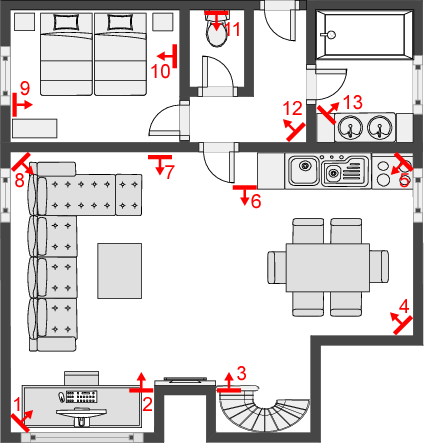
\includegraphics[scale=0.35]{img/SINS_database_floor_map.png}
	\caption[SINS database recording environment map]{SINS database recording environment map \footnotemark}
	\label{fig:sins-database-floor-map}
\end{figure}
\footnotetext{\href{https://www.semanticscholar.org/paper/THE-SINS-DATABASE-FOR-DETECTION-OF-DAILY-ACTIVITIES-Dekkers-Lauwereins/de84995b6b0042c9f6f1ccbd1f13d75b14c24e80/figure/1}{\nolinkurl{semanticscholar.org/paper/THE-SINS-DATABASE-FOR-DETECTION-OF-DAILY-ACTIVITIES-Dekkers-Lauwereins}}}
\noindent
One person lived in the environment for a continuous duration of one week. In order to have an as realistic as possible data recording, there was no predefined set of scenarios. Due to that, the recorded activities also included being absent from the home. Although there were no restrictions on the actions, the number of activities that were labelled was limited, as indicated in table \ref{tab:sins-database-recorded-activities} of the appendix \ref{app:SINS-Databse-Table}. In total there are 16 different recorded activities in five different rooms. Table \ref{tab:sins-database-recorded-activities}, which can be found in the appendix \ref{app:SINS-Databse-Table}, lists the different activities along with the number of examples and the mean and standard deviation and the duration of all examples for each room.

\subsection[DCASE 2018 Challenge - Task 5 dataset]{DCASE 2018 Challenge - Task 5: Monitoring of domestic activities based on multi-channel acoustics \footfullcite{dekkers_dcase_2018}}
\label{sub:DCASE-Task-Dataset}
This subsection contains all the necessary information about the challenge from the IEEE AASP Challenge on \gls{DCASE} 2018. The challenge finished in 2018, and the results, as well as the full dataset, were published. The main goal of the challenge was to classify multi-channel audio segments into predefined classes and determine how beneficial multi-channel recordings are for classification. 

\begin{figure}[htbp]
	\centering
	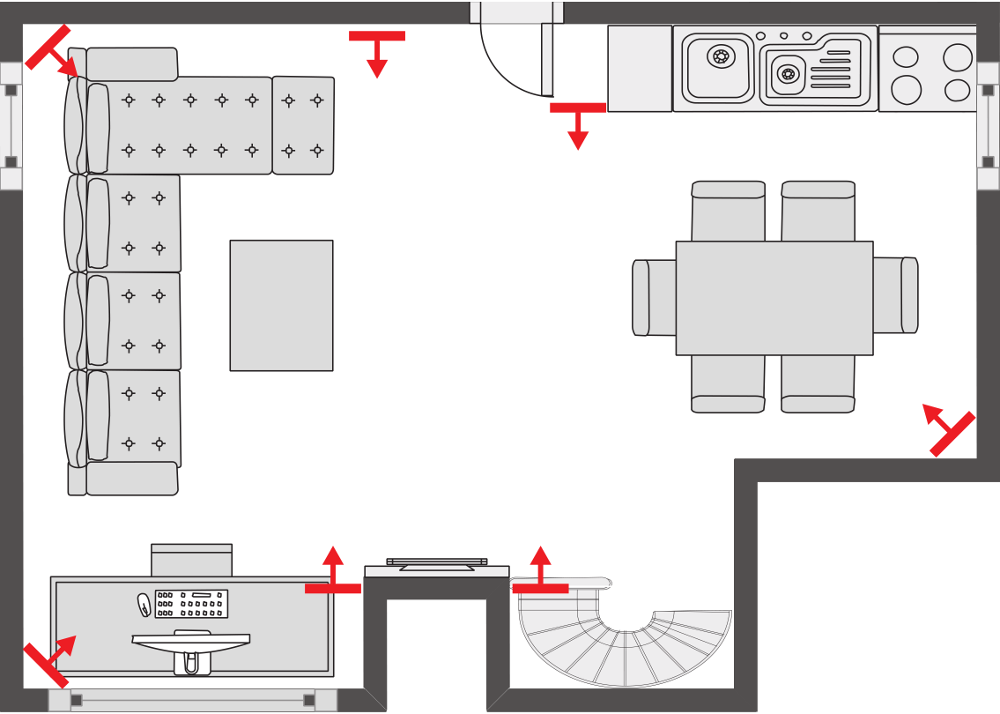
\includegraphics[scale=0.8]{img/DCASE_floor_map.png}
	\caption[2D floor plan of the combined kitchen and living room from DCASE]{2D floor plan of the combined kitchen and living room with the used sensor nodes \footnotemark}
	\label{fig:dcase-recordings-floor-plan}
\end{figure}
\footnotetext{\href{http://dcase.community/challenge2018/task-monitoring-domestic-activities}{\nolinkurl{dcase.community/challenge2018/task-monitoring-domestic-activities}}}
\noindent
The dataset used in the challenge is an abbreviation of the \nameref{sub:SINS-Database}; where only seven of the thirteen microphone nodes were considered. These nodes are from the room combination of the living room and the kitchen, as illustrated in figure \ref{fig:dcase-recordings-floor-plan}. Every recording of an activity is split into ten-second recordings, which are called segments. Every segment has four channels which correspond to the four different microphone channels of each node. Within the dataset, there are no overlapping sounds, from actions performed simultaneously. That means that every segment has an activity label assigned to it. There are a total of nine different activity labels, which all refer to a daily activity performed at home. Table \ref{tab:DCASE-activiies-performed} shows the activities performed in the dataset as well as the amount of 10 second segments and sessions of the activity.
\newline
\newline
In the challenge, the data was split into a development and an evaluation set. The development set is used for training the model and was made available for everyone participating in the challenge. It contains four of the seven microphone nodes which are 200h of audio data. This dataset also contains the corresponding label to each audio segment. The evaluation set is used for evaluating the final models to see their performance on never seen before data from the other three nodes. A session of an activity is a full recording of an action. Within both of these datasets, each session was kept together.
\begin{table}[htbp]
    \centering
    \caption[Activities performed in the dataset proposed by DCASE]{Activities performed in the dataset proposed by DCASE \footnotemark}
	\label{tab:DCASE-activiies-performed}
    \begin{tabular}{l|l|l}
        \toprule
        \textbf{Activity performed} & \textbf{\# 10s segments} & \textbf{\# sessions} \\ 
        \midrule[1pt]
        Absence (nobody present in the room) & 18860 & 42 \\
        \hline
        Cooking & 5124 & 13 \\ 
        \hline
        Dish washing & 1424 & 10 \\ 
        \hline
        Eating & 2308 & 13 \\ 
        \hline
        Other (present, but not doing any relevant activity) & 2060 & 118 \\ 
        \hline
        Social activity (visit, phone call, ...) & 4944 & 21 \\ 
        \hline
        Vacuum cleaning & 972 & 9 \\ 
        \hline
        Watching TV & 18648 & 9 \\ 
        \hline
        Working (typing, mouse clicking, ...) & 18644 & 33 \\ 
        \midrule[1pt]
        \textbf{Total} & \textbf{72984} & \textbf{268} \\
        \bottomrule
    \end{tabular}
\end{table}
\footnotetext{\href{http://dcase.community/challenge2018/task-monitoring-domestic-activities}{\nolinkurl{dcase.community/challenge2018/task-monitoring-domestic-activities}}}

\subsection{Music dataset}
\label{sub:Music-Dataset}

The second dataset used within the thesis is the music, which consists of songs classified by their respective genre. The songs are classified by the genre, according to \url{beatport.com}, which is an electronic music-oriented online music store. Beatport is oriented primarily towards DJs, selling full songs as well as resources which can be used for remixes. Each genre consists of 30 different songs, which vary heavily in length, from 3min up to 10min. The dataset contains approximately 18 hours of music provided as a single channel mp3 files. Table \ref{tab:Music-Dataset} shows the genres from the dataset along with the number of songs within each.

\begin{table}[htbp]
    \centering
    \caption{Music genres in the music dataset along with the number of songs}
	\label{tab:Music-Dataset}
    \begin{tabular}{p{.70\textwidth} | p{.20\textwidth}}
        \toprule
        \textbf{Music genres} & \textbf{\# songs} \\ 
        \midrule[1pt]
        Deep House & 30 \\
        \hline
        Electronica Downtempo & 30 \\ 
        \hline
        Indie Dance & 30 \\ 
        \hline
        Melodic House and Techno & 30 \\ 
        \hline
        Techno Peak Time Driving Hard & 30 \\ 
        \hline
        Techno Raw Deep Hypnotic & 30 \\ 
        \hline
        Trance & 30 \\
        \midrule[1pt]
        \textbf{Total} & \textbf{210} \\
        \bottomrule
    \end{tabular}
\end{table}

\section{State of the art}
\label{sec:State-of-art}
Within this section of the thesis, two state-of-the-art concepts are introduced, which will be essential for the following chapters and used throughout the whole project. Therefore it is essential to be familiar with the terms, definitions and equations of \nameref{sub:Triplet-Loss} and \nameref{sub:Tile2Vec}. First \nameref{sub:Triplet-Loss} will be introduced, and after that, the \nameref{sub:Tile2Vec} concept, which is an application of the \nameref{sub:Triplet-Loss}.

\subsection{Triplet Loss}
\label{sub:Triplet-Loss}

Triplet loss was first introduced in the field of face recognition by the paper (\cite{schroff_facenet_2015}) from Google. They describe a new approach to train face embeddings using online triplet mining.
\begin{figure}[htbp]
	\centering
	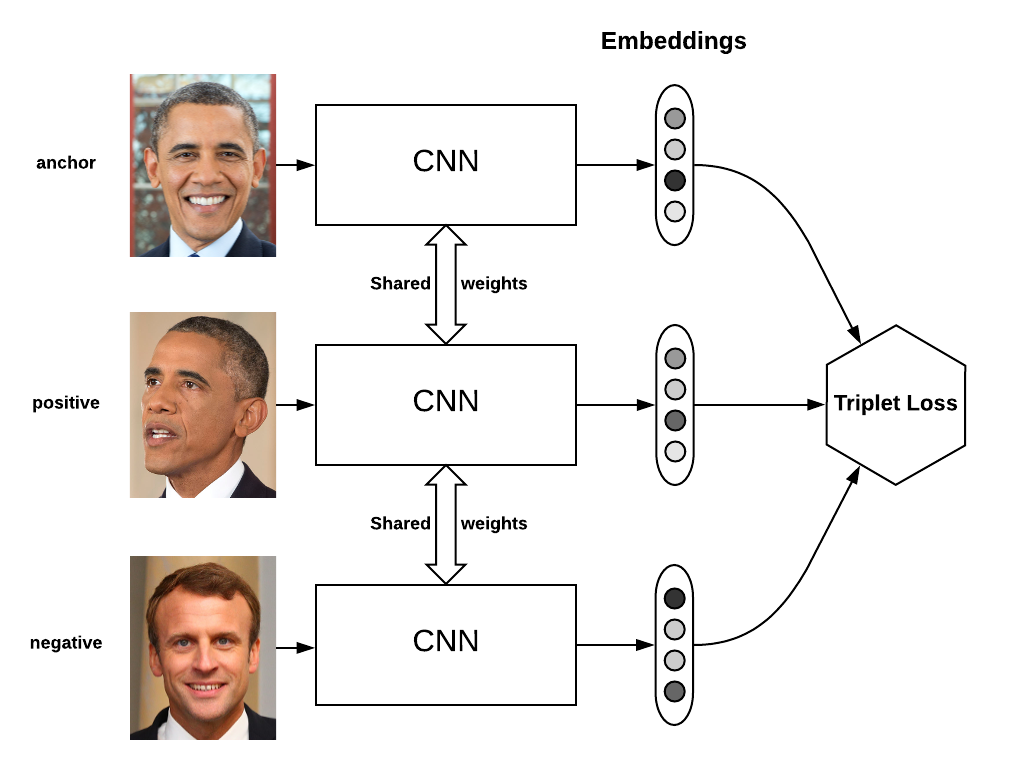
\includegraphics[scale=0.35]{img/Triplet_Loss_Architecture.png}
	\caption[Triplet Loss architecture visualisation]{Triplet Loss architecture visualisation \footnotemark}
	\label{fig:Triplet-Loss-Architecture}
\end{figure}
\footnotetext{\url{https://omoindrot.github.io/triplet-loss}}
\noindent
\myequations{Euclidean distance}
\begin{equation}
    \centering
    \begin{gathered}
        d(p,q) = \big|\big|q-p\big|\big|_2 = \sqrt{(q_1 - p_1)^2 + \dots + (q_n - p_n)^2} = \sqrt{\sum_{i=1}^n (q_i - p_i)^2}
    \end{gathered}
    \label{eq:Euclidean-Distance}
\end{equation}
\noindent
The introduced architecture helps to learn distributed embeddings by the notion of similarity and dissimilarity. Within the neural network architecture, multiple parallel networks are trained, which share the same weights among each other; this is illustrated in figure \ref{fig:Triplet-Loss-Architecture}. The objective is to build triplets consisting of an anchor $x_a$, a positive $x_p$ and a negative sample $x_n$. Where the positive sample is similar to the anchor and the negative one is dissimilar to the anchor. In the high dimensional vector space, contextually similar data points are projected in the near-by region ($x_a$ and $x_p$). In contrast, different data points are projected far away from each other ($x_a$ and $x_n$). This condition is defined by the equation \ref{eq:Triplet-Loss-Constraint}. Where $|| \cdot ||_2$ is defined as the euclidean distance with equation \ref{eq:Euclidean-Distance} and $\tau$ is the set of all possible triplets in the dataset.
\myequations{Triplet Loss constraint}
\begin{equation}
    \centering
    \begin{gathered}
        \Big|\Big|f_\theta(x_a) - f_\theta(x_p)\Big|\Big|_2^2 + \alpha < \Big|\Big|f_\theta(x_a) - f_\theta(x_n)\Big|\Big|_2^2 \\[10pt]
        \forall \big(f_\theta(x_a), f_\theta(x_p), f_\theta(x_n)\big) \in \tau
    \end{gathered}
    \label{eq:Triplet-Loss-Constraint}
\end{equation}
The embedding of a given sample $x$ is represented by $f_\theta(x) \in \mathbb{R}^d$, where $f$ is a some kind of network (e.g. fully connected \gls{NN}, \gls{CNN}, \gls{RNN}, or any other) with weights $\theta$. It embeds a sample $x$ into a $d$-dimensional Euclidean space. The loss, which will be minimised, is defined by the equation \ref{eq:Triplet-Loss}. Where $\alpha$ is a margin that is enforced between positive and negative pairs, it further puts a limit on how far the network can push the negative sample away to improve the loss. In equation \ref{eq:Triplet-Loss}, the notation $[\cdot]_+$ is used to represent the rectifier $\text{max}(0, \cdot)$.
\myequations{Triplet Loss function}
\begin{equation}
    \centering
    \mathcal{L} = \Bigg [\Big|\Big|f_\theta(x_a) - f_\theta(x_p)\Big|\Big|_2^2 - \Big|\Big|f_\theta(x_a) - f_\theta(x_n)\Big|\Big|_2^2 + \alpha \Bigg]_+
    \label{eq:Triplet-Loss}
\end{equation}
When the loss is minimised, it pushes the distance between $f_\theta(x_a)$ and $f_\theta(x_p)$ near zero. Contrarily it forces the distance between $f_\theta(x_a)$ and $f_\theta(x_n)$ to be higher than the distance between $f_\theta(x_a)$ and $f_\theta(x_p)$ plus some margin $\alpha$.
\newline
\newline
Generating all possible triplets of a dataset would result in many triplets which easily satisfy the equation \ref{eq:Triplet-Loss-Constraint}. These easy triplets would not contribute to the training and result in slower convergence, as they would still be passed through the network. Therefore it is crucial to select only hard triplets, which can enhance the model. This means that given $x_a$, $x_p$ is selected to be a hard positive such that equation \ref{eq:Triplet-Loss-Hard-Positive} is satisfied. Similarly, $x_n$ is a hard negative when equation \ref{eq:Triplet-Loss-Hard-Negative} is fulfilled. However, it is probably not feasible to make these calculations for the whole dataset, because they are computing-intensive. Nevertheless, it can be used to improve the model, for example, to better distinguish between classes which are quite similar.
\myequations{Triplet Loss hard positive}
\begin{equation}
    \centering
    \text{hard positive} = \text{argmax}_{x_p} \ \Big|\Big|f_\theta(x_a) - f_\theta(x_p)\Big|\Big|_2^2
    \label{eq:Triplet-Loss-Hard-Positive}
\end{equation}
\myequations{Triplet Loss hard negative}
\begin{equation}
    \centering
    \text{hard negative} = \text{argmin}_{x_n} \ \Big|\Big|f_\theta(x_a) - f_\theta(x_n)\Big|\Big|_2^2
    \label{eq:Triplet-Loss-Hard-Negative}
\end{equation}

\subsection{Tile2Vec}
\label{sub:Tile2Vec}

Tile2Vec was first introduced by the paper (\cite{jean_tile2vec_2018}) from Stanford University. It is an unsupervised representation learning algorithm that extends the distributional hypothesis from natural language to spatially distributed data. This hypothesis implies that words appearing in similar contexts tend to have similar meanings. Tile2Vec is used to learn compressed yet informative representations from unlabeled remote sensing data.
\newline
\newline
In the cited paper, the main focus is on remote sensing, which is the measurement of the Earth's surface through aircraft- or satellite-based sensors. In remote sensing, the biggest problem is the scarcity of labelled data. Thus the use of unsupervised machine learning is necessary. Hereafter the data, which is used to train the algorithm, consists of geospatial tiles.
\newline
\newline
The distributional hypothesis in linguistics is the idea that \flqq a word is characterised by the company it keeps\frqq. In \gls{NLP}, algorithms like Word2Vec and GloVe leverage this assumption to learn continuous representations that capture the nuanced meanings of vast word vocabularies.
\newline
\newline
Tile2Vec proposes to learn the representations on the level of remote sensing tiles, a generalisation of image patches to multi-spectral data. The context of each tile relies on the spatial neighbourhood, which is defined as some distance in the geographic space. The assumption is that tiles which are located close together have a similar meaning and should, therefore, have similar representations in the embedding space.
\newline
\newline
To learn a mapping from image tiles to low-dimensional embeddings, a \gls{CNN} is trained on triplets of tiles, where each triplet consists of an anchor tile $x_a$, an adjacent tile $x_p$ which is geographically close and a distant tile $x_n$ which is farther away. Following the distributional assumption, the Euclidean distance (eq. \ref{eq:Euclidean-Distance}) between the embedding of the anchor tile and the neighbour tile is minimised, while maximising the distance between the anchor and distant embedding (\nameref{sub:Triplet-Loss}). For each tile triplet $(x_a, x_p, x_n)$ the triplet loss (\ref{eq:Triplet-Loss}) is therefore minimized.
\newline
\newline
But when $||f_\theta(x_a) - f_\theta(x_p)||_2 < ||f_\theta(x_a) - f_\theta(x_n)||_2$, all embeddings can be scaled by some constant in order to satisfy the margin and bring the loss to zero. After a small number of iterations, the \gls{CNN} learns to increase the embedding magnitudes to decrease the loss to zero. By penalising the embeddings $l^2$-norms, the network is forced to generate embeddings within a hypersphere, leading to a representation space in which relative distances have meaning. The regularisation term is defined by $\lambda \Big(||f_\theta(x_a^{(i)})||_2 + ||f_\theta(x_p^{(i)})||_2 + ||f_\theta(x_n^{(i)})||_2\Big)$, which can be controlled using the hyperparameter $\lambda$. The cost function of the Tile2Vec algorithm is defined by equation \ref{eq:Tile2Vec-Cost-Function}. Where $N$ is the cardinality of the valid triplets in the dataset and $\mathcal{L}$ is the triplet loss (\ref{eq:Triplet-Loss}).
\myequations{Tile2Vec Cost function}
\begin{equation}
    \centering
    \min_\theta \sum_{i=1}^N \Bigg[\mathcal{L}\Big(x_a^{(i)}, x_p^{(i)}, x_n^{(i)}, \theta\Big) + \lambda \Big(||f_\theta(x_a^{(i)})||_2 + ||f_\theta(x_p^{(i)})||_2 + ||f_\theta(x_n^{(i)})||_2\Big)\Bigg]
    \label{eq:Tile2Vec-Cost-Function}
\end{equation}
The sampling procedure for the triplet $(x_a, x_p, x_n)$ is described by two parameters, the tile size and the neighbourhood radius. The tile size defines the pixel width and height of a single tile. The neighbourhood radius defines the region around the anchor tile from which to sample the adjacent tile. The centre of the neighbour tile must be within this radius of the anchor, and the distant tile is then sampled at random from outside the radius.

\section{Status in relation to project}
\label{sec:Status-Relation-Project}

This section of the chapter focuses on the current state of the art deep learning techniques for audio signal processing, which are relevant for this project. Many of these techniques were first introduced for the field of image processing and then adapted for audio processing. However, there is a vast difference between image and audio data, for example, raw audio data samples from a one-dimensional time-series signal, whereas image data is two-dimensional. Thus many of the traditional techniques had to be adapted for audio data.
\newline
\newline
This thesis considers its main task to be a \textit{sequence classification}, where a single global class label needs to be predicted for an audio sequence. However, there is no defined terminology for deep learning with audio. Thus there are many variant terms in use.
\newline
\newline
\fullref{sub:Mel-Spectrogram} is the most common representation used in traditional audio signal processing, log-mel spectrograms are the dominant feature in deep learning, followed by raw waveforms or complex spectrograms. Raw waveforms avoid hand-designed features, which should allow better to exploit the improved modelling capability of deep learning models. However, this incurs higher computational costs and data requirements, and the benefits are hard to realize in practice. For \gls{ASR}, log-mel spectrograms provide a more compact representation, and methods using these features usually need fewer data and training to achieve results, which are comparable in performance to a setup where raw audio is used. \gls{MFCC} and log-mel spectrograms are gladly used because they were inspired by the human auditory system, which makes the use of these features reasonable.
\newline
\newline
Across many audio processing domains, \fullref{sub:Convolutional-Neural-Network}, \gls{RNN} and \gls{CRNN} are employed successfully, with no clear preference. All three can model temporal sequences, solve sequence classification and many more applications. \gls{CNN} have a fixed receptive field, which limits the temporal context taken into account for a prediction, but at the same time makes it very easy to widen or narrow the context used. The receptive field can be increased using larger kernels or stacking more layer. Alternatively, another way to increase the receptive field of a \gls{CNN} is to stack dilated convolution layers (\ref{subsub:Dilated-Convolution}), which apply the convolution filter over an area larger than its filter length. These convolutions obtain a vast receptive field with just a few layers while preserving the input resolution as well as computational efficiency (\cite{franceschi_unsupervised_2020}).
\newline
\newline
\gls{RNN} can, theoretically, base their predictions on an unlimited temporal context, but first need to learn to do so, which may require adaptions to the model (such as \fullref{sub:Gated-Recurrent-Unit}). Furthermore, they require processing the input sequentially, making them slower to train and evaluate than \gls{CNN}. \gls{CRNN} offer a compromise in between, inheriting both \gls{CNN} and \gls{RNN} advantages and disadvantages.
\newline
\newline
Thus the process of choosing the superior model for a specific task is still an open research question. From existing literature, this is very hard to answer, since the different research groups yield state-of-the-art results with different models. This may be due to each research group’s specialized informal knowledge about how to design and tune a particular architecture type effectively. \footnote{\fullcite{purwins_deep_2019}}
\newline
\newline
With the possible exception of speech recognition, in the industry, for the most popular languages, all tasks in all audio domains face relatively small datasets, posing a limit on the size and complexity of deep learning models trained on them. However, in other domains, such as computer vision the shortage of labelled data for a particular task is offset by the widespread availability of models trained on the ImageNet dataset. Nevertheless, no comparable task and dataset exist for the audio domain.
\newline
\newline
Most of the models submitted in the \fullref{sub:DCASE-Task-Dataset} used \gls{MFCC} or log-mel spectrograms as acoustic features along side with a \gls{CNN} as their main architecture. The winner of the challenge was the IBM research team, which show their model in the paper (\cite{inoue_domestic_2018}). They only used the input data provided in the dataset, from the challenge, and sampled it at a rate of 16kHz. From the dataset, the log-mel energies (\ref{sub:Mel-Spectrogram}) are extracted and used to train a \gls{CNN}. They propose data augmentation techniques using shuffling and mixing two sounds in the same class, to mitigate the unbalanced training dataset. Which led them to train their model on a much larger dataset than the rest.
\newline
\newline
Another model in the challenge, proposed in the paper (\cite{liu_ensemble_2018}), uses an ensemble of a \gls{CNN} and a \gls{RNN} to achieve some remarkable results without any data augmentation. 

\chapter{Ideas and concepts}
\label{ch:Ideas-Concepts}
This chapter explains the different ideas and concepts used to realise the thesis. Some ideas were discovered during the research and were already introduced in the sections of related work (\ref{ch:Related-Work}) or were introduced in other approaches (\ref{sec:Other-Approaches}). Others were developed especially for this project and their application, as well as their advantages, will be proven in this work.
\newline
\newline
It is important to know that in the thesis, two distinct datasets are used to evaluate the application of the developed architecture in two domains. Due to that, many of the sections in this chapter are divided into two groups, one for the \fullref{sub:DCASE-Task-Dataset} and one for the music dataset (\ref{sub:Music-Dataset}).

\section{Data preprocessing}
\label{sec:Data-Preprocessing}
Data preprocessing is the process of processing the entire dataset before it is fed into the input pipeline (\ref{sec:Input-Pipeline}), either manually or automatically. Both datasets used in the project consist of audio files, which are grouped together by their corresponding label. Thus the structure of both datasets is very similar. For this thesis, it was decided that data preprocessing was not necessary for the \fullref{sub:DCASE-Task-Dataset}. However, for the music dataset (\ref{sub:Music-Dataset}), a minimal manual preprocessing is needed to improve the performance of the pipeline.
\newline
\newline
The \fullref{sub:DCASE-Task-Dataset} was already preprocessed by the organisers of the challenge. Which means that there are no audio files which contain multiple labels, are corrupted or invalid. The organisers of the challenge further split the sessions of recordings into 10s samples, which provides an easy and fast to use dataset. Therefore the preprocessing is neglected.
\newline
\newline
The music dataset (\ref{sub:Music-Dataset}) consists of different songs grouped by their respective genre. The audio samples in this dataset are given in the format of \texttt{.mp3} files, which is not that fast to process as for example \texttt{.wav} formatted audios. Therefore all of the \texttt{.mp3} audios were converted using \texttt{ffmpeg} to \texttt{.wav} files, with the simple script \ref{code:Convert-mp3-wav}.
\begin{code}[htbp]
\begin{minted}{bash}
for i in *.mp3; 
do ffmpeg -i "$i" "${i%.*}.wav";
done;
\end{minted}
\caption{Convert \texttt{.mp3} files to \texttt{.wav} files using \texttt{ffmpeg}}
\label{code:Convert-mp3-wav}
\end{code}
Further, the audios of the music dataset will be trimmed within the input pipeline (\ref{sec:Input-Pipeline}), because they should not contain any silence at the start or end of a song since this could lead to misclassified segments and clusters of silence, which should be omitted.

\section{Feature extraction}
\label{sec:Feature-Extraction}
Feature extraction, sometimes called feature representation, is the process of extracting the relevant features from the raw data; in this case, audio files. The extraction process is done within the input pipeline (\ref{sec:Input-Pipeline}). For both datasets, the same feature representations are used. Three different extractions are evaluated and are used as a hyperparameter which can be tuned to achieve the best possible performance. The optimal feature representation for the two datasets may be different since their characteristics are quite different. However, research has to show if that is the case.
\newline
\newline
The first approach is to use the audio files as they are, more precisely to use the raw waveform as input to the model. This is the most straightforward approach and as well the most lightweight to compute. It will be used to evaluate how good a model can be trained without any further feature extraction. The approach to use the raw waveform would be the simplest one to implement in a real-world application, because there is no complex computation needed, and can therefore as well be used on small devices, such as mobile phones or Raspberry Pis. However, when using the raw waveform of an audio segment, the preprocessing task of the input pipeline will get omitted, but the model gets a lot bigger since the input size is much larger than when using a feature representation. For example, when using the raw waveform of a 10s segment with the sample rate of 16'000, the input size gets 160'000, which is very large in comparison to the size when using a feature representation.
\newline
\newline
The second approach is to calculate the log-Mel spectrogram, which is outlined in subsection Mel spectrogram (\ref{sub:Mel-Spectrogram}), where the last step of calculating the \gls{DCT} is omitted. The process described was introduced to mimic the human hearing, but the last step, calculating the \gls{DCT}, was proposed because many machine learning models struggled with the highly correlated data, such as the log-Mel spectrogram, and thus a linear transformation (\gls{DCT}) was added to decorrelate the feature. Contemporary machine learning models such as \glspl{CNN} or \glspl{GRU} do not struggle with correlated data and perform even better when they can decorrelate the features themselves. Therefore this approach should give useful insight, weather the decorrelation can be trained and is still needed in present models. This approach is widely used in the audio domain because it is less computing extensive than calculating the \glspl{MFCC} and it can achieve almost the same, or an even better, accuracy as a model trained with the \glspl{MFCC} as their feature representation because it uses the same computations and additionally preserves more information.
\newline
\newline
The third and final approach is to calculate and use the \glspl{MFCC}, which is described in subsection Mel spectrogram (\ref{sub:Mel-Spectrogram}). This feature extraction method is used mainly in extensive audio applications, such as automatic speech and speaker recognition, where a lot of computing power is available. These features are mostly used because of their nature, that they represent sound like the human auditory system does, in a compact matter.
\newline
\newline
All of the features stated above are two-dimensional data, and therefore, standard image processing architectures can be adapted to audio processing. This adaption of image processing architectures to audio has successfully be shown in recent years of research \footcite{dai_acoustic_2016} \footcite{takahashi_deep_2016} \footcite{purwins_deep_2019} \footcite{lee_samplecnn_2018} \footcite{pons_timbre_2017}. 

\section{Triplet selection}
\label{sec:Triplet-Selection}
The triplet selection describes the process of selecting a neighbouring and opposite sample from a given anchor sample. The idea of triplet selection and the motivation behind it is described within section triplet loss (\ref{eq:Triplet-Loss}). The procedure is split into two parts, the selection of the neighbouring and opposite tile.
\newline
\newline
The straightforward way to triplet selection, as described in \ref{eq:Triplet-Loss}, is to select the anchor and the neighbour to be part of the same label and to select the neighbour to have a different label than the other. However, this approach can not be used in an unsupervised learning technique because the data does not have any information about the underlying label. Due to that, a different, unsupervised approach to triplet selection has to be chosen.
\newline
\newline
For the triplet selection of the \fullref{sub:DCASE-Task-Dataset}, all of the 10s audio files have to be first split into a specified \textit{sample length} (e.g. 1s, 2s). This results in different segments belonging to the same audio file, which are referred to as segments and denoted as $x$. The sample length specifies the length of all the segments. Therefore a triplet consists of three different segments $(x_a, x_n, x_o)$.
\newline
For the anchor tile $x_a$, a random segment is chosen. For the neighbouring tile $x_n$, a segment will be selected which belongs to the same audio file as the anchor, where the selection has to be done within a predefined range, \textit{neighbouring selection range} (e.g. 2s, 4s), of the anchor tile $x_a$. It is important to note, that it does not make any difference if the tile is being sampled from before or after the anchor segment. The segments $x_a$ and $x_n$ have to be distinct from each other and chosen within the specified \textit{neighbouring selection range}.
\newline
The opposite tile $x_o$ will be chosen at random from a different audio sample, where the selection of the segment is as well performed at random. The only constraint is that the opposite tile can not be chosen from the same audio file as the anchor and the neighbour.
\newline
\newline
For the music dataset (\ref{sub:Music-Dataset}), the triplet selection is made relatively similar to the one described in the paragraph above for the \fullref{sub:DCASE-Task-Dataset}. The only difference between the two methods is that for the music dataset, the audio files are of variable length. However, this does not make any difference in the selection process. The only difference between the two methods is that maybe the \textit{sample length} and \textit{neighbouring selection} range will need to be increased due to the increased audio file length, but this has to be shown in the experiments.

\section{Input pipeline}
\label{sec:Input-Pipeline}
\begin{figure}[htbp]
	\centering
	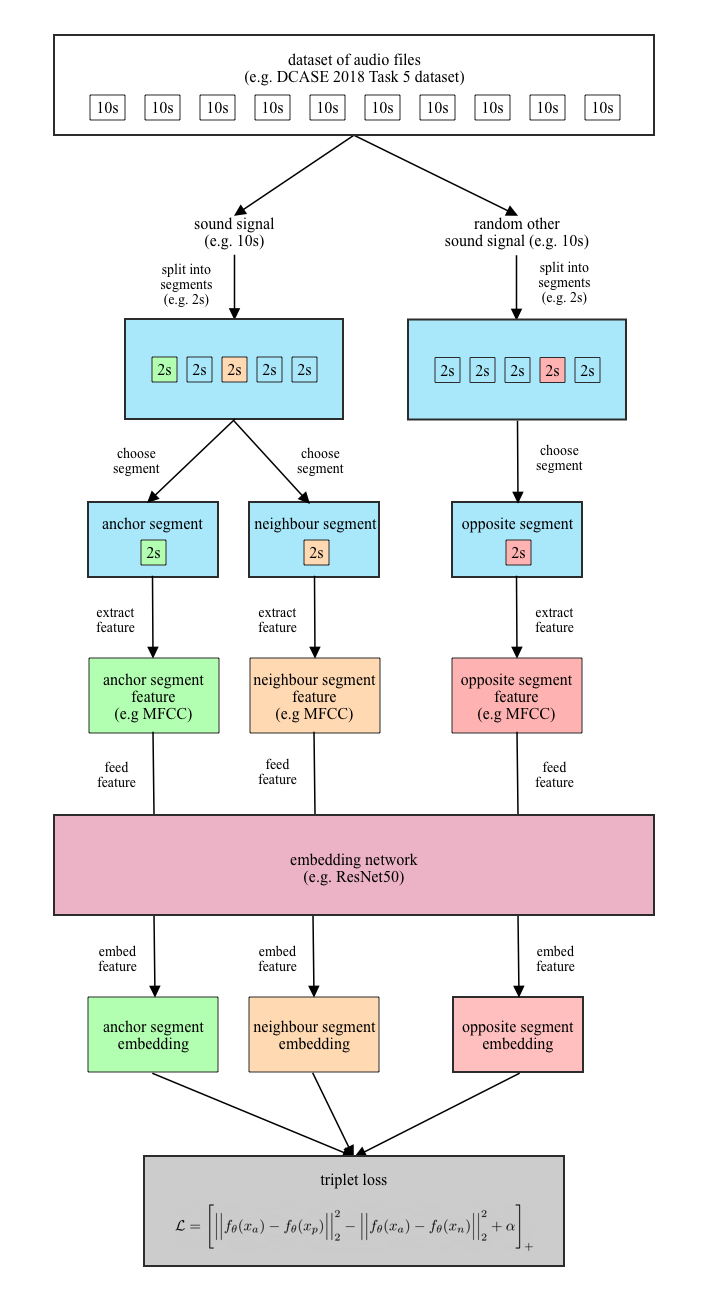
\includegraphics[scale=0.4]{img/Input_Pipeline_Visualisation.png}
	\caption{Visualisation of the input pipeline process}
	\label{fig:Input-Pipeline-Visualisation}
\end{figure}
\noindent
The input pipeline is responsible for creating the dataset, which will then be fed into the model by batches. For this project, the input pipeline is implemented using the TensorFlow \texttt{tf.data} API\footnotemark, along with a generator, which loops over the whole dataset and creates entries on the fly. The reason why a generator function is used, is that the entire dataset can not be loaded into memory, due to the large size of it. The entire process of the input pipeline is illustrated in figure \ref{fig:Input-Pipeline-Visualisation}.
\footnotetext{\url{https://www.tensorflow.org/api_docs/python/tf/data}}
\newline
\newline
The feature extraction (\ref{sec:Feature-Extraction}) and the triplet selection (\ref{sec:Triplet-Selection}) of the audio files is done on the fly within the input pipeline (\ref{sec:Input-Pipeline}). The advantage of this method is that the pipeline can be adapted fairly quick for other datasets since the only input the pipeline requires is the raw waveform of any audio signal.
\newline
\newline
The first step of the input pipeline is to loop over the corresponding generator function of the specified dataset, which loops over the entire dataset and returns the current sample of the dataset. For each one of the returned samples, a triplet, consisting of an anchor, neighbour and an opposite audio segment, is created by using the datasets method to perform the selection. The triplet, which will be returned from the dataset consists of indices of the audio and segment for each one of the three segments. Then the input pipeline uses these indices to extract the corresponding audio segment out of the dataset and yields them back to the \texttt{tf.data.Dataset}. It is important to note that all the operations listed after this paragraph are done on the whole batch.
\newline
\newline
After the dataset gets an entire batch of audio segments, the feature extraction will be performed. The feature extraction is implemented using the vectorised \texttt{.map} function of the class \texttt{tf.data.Dataset}\footnotemark. The \texttt{.map} function applies a given function to each element within the dataset, which in the case of this thesis, will be used to extract the features from the audio. Hence a \flqq feature extractor\frqq \ has to be provided to the input pipeline, which will extract a certain feature from the audio as stated in \ref{sec:Feature-Extraction}. If no extractor is passed to the pipeline, the raw waveform of the signal is used. 
\footnotetext{\url{https://www.tensorflow.org/api_docs/python/tf/data/Dataset}}
\newline
\newline
After the extraction, the dataset is shuffled and returned to the training process. In the training loop, the dataset can now be iterated over, which yields back a batch of triplets, consisting of the extracted audio segment. This batch can then be used to train the model. The dataset is therefore similar to a Python iterator.
\newline
\newline
The advantages of this method are that this creates the dataset dynamically, because the dataset only contains the current batch along with some prefetched entries, which are entries from the next batch so that the \gls{GPU} can be fully utilised.

\section{Models}
\label{sec:Models}
This section describes the overall architecture of the models used in the thesis. The idea of the thesis is to evaluate different kinds of architectures and compare their results to find the optimal model for the thesis.
\newline
\newline
The first architecture, which will be evaluated are \glspl{CNN} (\ref{sub:Convolutional-Neural-Network}). They are used in a lot of audio applications because of their simplicity and robustness. A considerable amount of research in the past couple of years has shown the overall success of these models. Therefore it makes sense to evaluate these type of models extensively. Subsection \ref{sub:ResNet} describes a state-of-the-art \gls{CNN} architecture, which will be mainly used throughout the thesis.
\newline
\newline
Another widely used model architecture is the \gls{RNN}, where \glspl{GRU} (\ref{sub:Gated-Recurrent-Unit}) are one of the most prominent implementations. Their application primarily lies in the text-domain. However, in recent years they have shown their success within the audio domain, mainly because of the sequential nature of the audio signal.
\newline
\newline
The most prominent approach in audio research is the combination of \glspl{CNN} and \glspl{RNN}. The architecture consists of multiple convolution layers, and a single or multiple recurrent layers. The idea of these models is that they first reduce the input data to a specific lower-dimensional representation and then use recurrent models to make use of the sequential nature of the audio. Therefore the best ideas of both architectures are used within these \glspl{CRNN}.
\newline
\newline
For the implementation and the experiments, \glspl{CNN} should be mainly used, and if there is time, to evaluate and implement state-of-the-art \gls{RNN} and \gls{CRNN} models.

\subsection{ResNet}
\label{sub:ResNet}
\Gls{ResNet} is a state-of-the-art \gls{CNN} architecture, which was introduced in 2015 (\cite{he_deep_2015}), and was the winner of ImageNet Visual Recognition Challenge 2015. The problem \gls{ResNet} solves is the degradation problem, which has been observed when deeper networks start converging. The problem states, that with the network depth increasing, accuracy gets saturated and then degrades rapidly. Therefore, using deeper networks is degrading the performance of the model. \cite{he_deep_2015} tries to solve this problem using deep residual learning framework. The core idea introduced are so-called \flqq identity shortcut connection\frqq \ that skip one or more layers, as shown in figure \ref{fig:ResNet-Residual-Block}. Typical \gls{ResNet} models are implemented with double- or triple- layer skips that contain non-linearities (ReLU) and batch normalization in between, as shown in figure \ref{fig:ResNet-Skip-Layers}. The whole architecture is a stack of residual blocks with appropriate stride and pooling. These residual networks are easier to optimise and can gain accuracy from considerably increased depth. They have shown their applicability in much research in recent years and should, therefore, be used as the main model architecture throughout this thesis.
\begin{figure}[htb]
\centering
\begin{subfigure}{.5\linewidth}
  \centering
  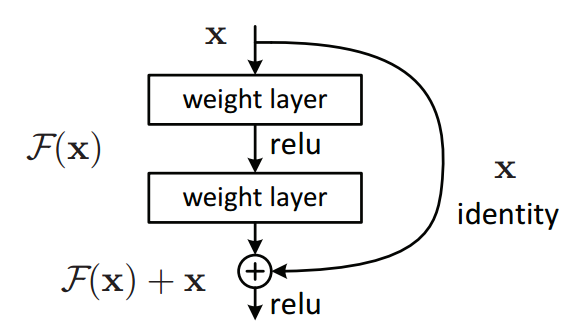
\includegraphics[width=\linewidth]{img/ResNet_SkipConnections.png}
  \caption{Residual block}
  \label{fig:ResNet-Residual-Block}
\end{subfigure}%
\begin{subfigure}{.5\linewidth}
  \centering
  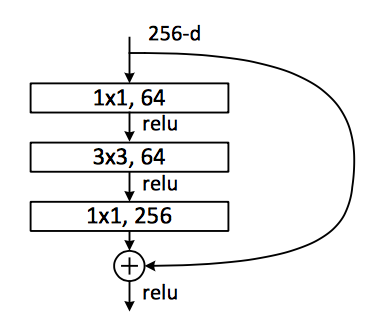
\includegraphics[width=.75\linewidth]{img/ResNet_Stacks.png}
  \caption{Triple layer skip connection}
  \label{fig:ResNet-Skip-Layers}
\end{subfigure}
\caption[ResNet visualisations]{ResNet visualisations\footnotemark}
\label{fig:ResNet-Visualisations}
\end{figure}
\footnotetext{\fullcite{he_deep_2015}}

\section{Application to music}
\label{sec:Application-Music}
All of the concepts mentioned above are designed to work with both datasets. Thus the application to music is described in each of the sections above separately. But to summarise, to adapt the model from the noise detection dataset to the music dataset, the same architecture will be used. This includes using the same triplet selection process. However, almost inevitably, the segments will need to be increased. Then to use the same input pipeline, with the same feature representation. This results in almost the same architecture as for the \gls{DCASE} dataset, with a few exceptions.

\section{Metrics}
\label{sec:Metrics}
Meaningful metrics need to be used to evaluate and compare the performance of machine learning models. In supervised machine learning, most of the metrics focus on how well the model predicts the actual value from the input, but in the unsupervised setting, finding meaningful metrics is a lot harder. Hence the metrics for the embedding model and the classifier are quite different because the embedding architecture is unsupervised while the classifier is supervised. Therefore this section is split into two parts, metrics for the embedding space (\ref{sub:Metrics-Embedding-Space}) and metrics for the classifier (\ref{sub:Metrics-Classifier}), which both aim to give valuable insights into the performance. All of the mentioned metrics below are monitored using the Tensorboard visualisation toolkit\footnote{\url{https://www.tensorflow.org/tensorboard}}.

\subsection{Embedding space}
\label{sub:Metrics-Embedding-Space}
As mentioned before, it is not easy to find meaningful metrics for the embedding space because of its unsupervised nature. However, since the thesis focuses on the application of triplet loss in the unsupervised setting, one of the most straight forward metrics to use is to monitor the triplet loss value, which gives insight if the model is training and learning a representation over time. Thus this value should be minimized over time. The triplet loss value, which will be monitored, results out of the equation \ref{eq:Triplet-Loss}. Since the idea of triplet loss is to minimize the distance between the anchor and the positive sample and to maximize the distance between the anchor and the negative sample, it makes sense to monitor them as well. Both values are already computed when computing the triplet loss and only have to be monitored. As a distance measure between the embeddings, the squared euclidean distance, given by equation \ref{eq:Euclidean-Distance}, is used. Monitoring these distances, give valuable insights if the model is capable of satisfying the triplet loss constraint or not. All of these three metrics are monitored both on the training and evaluation dataset.
\newline
\newline
The embedding space can further be thought of as a clustering task, where the goal is to cluster similar samples in the near-by region. Since the evaluation set contains the ground truth of each sample, most clustering metrics can be used to monitor the progress of the embedding space. 
\newline
\newline
One of the most straightforward metrics to use for evaluation and comparison of the resulting embedding spaces is the distances between the clusters. They can be computed by calculating the distance from each centroid of a cluster to every other. The metric gives an insight into how distant the clusters of each label are. It can be displayed in two different ways, as graphs and as a distance matrix in the form of an image. Such a representation in the form of an image is shown in figure \ref{fig:Distance-Matrix}. However, it is important to say that this metric is very vulnerable for outliers, which means that the centroid can vary very broadly if one of the clusters contains many outliers.
\newline
\newline
Further, a popular clustering metric called the silhouette coefficient, is used, where a higher score relates to a model with better-defined clusters. The score is bounded between $-1$ for incorrect clustering and $+1$ for highly dense clustering. Scores around zero indicate overlapping clusters. The score is higher when clusters are dense and well separated, which relates to a standard concept of a cluster. The silhouette coefficient is defined for each sample and is composed of two scores:
\begin{itemize}
\setlength\itemsep{0em}
    \item $a$: The mean distance between a sample and all other points in the same class
    \item $b$: The mean distance between a sample and all other points in the next nearest cluster
\end{itemize}
The silhouette coefficient $s$ for a single sample is then given by equation \ref{eq:Silhouette-Coefficient}. For a set of samples, the silhouette coefficient is given as the mean of the silhouette coefficient for each sample.
\myequations{Silhouette coefficient for a single sample}
\begin{equation}
    \centering
    \begin{gathered}
        s = \frac{b - a}{max(a, b)}
    \end{gathered}
    \label{eq:Silhouette-Coefficient}
\end{equation}
Both of the metrics above are only computed on the evaluation dataset, since monitoring it on the training set would not provide more insight.
\begin{figure}[htbp]
	\centering
	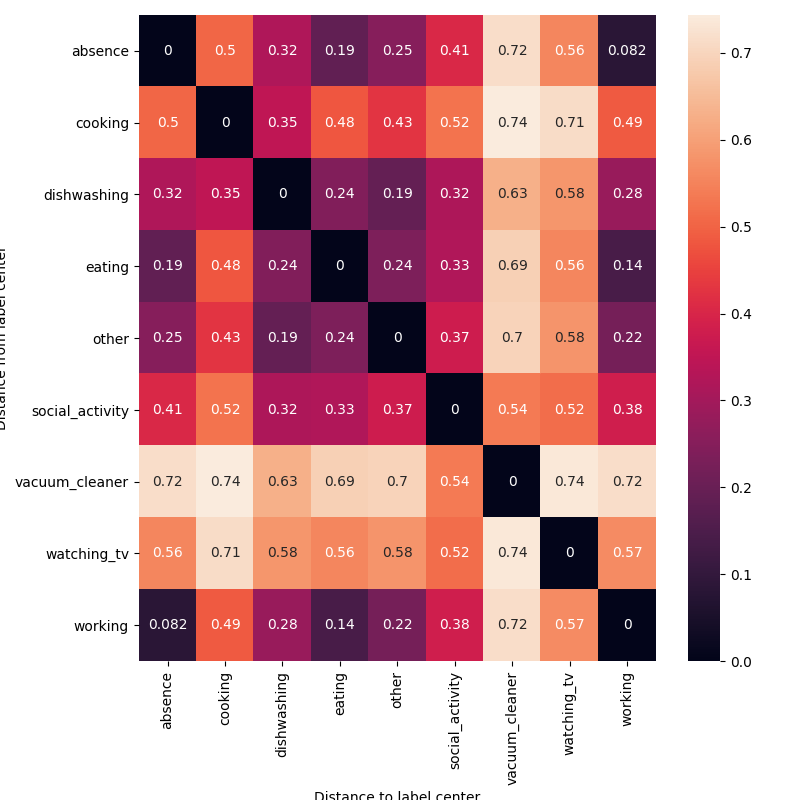
\includegraphics[scale=0.3]{img/Distance_Metric.png}
	\caption{Distance matrix from each centroid to every other}
	\label{fig:Distance-Matrix}
\end{figure}

\subsection{Classifier}
\label{sub:Metrics-Classifier}
For the classifier, standard supervised metrics are monitored, such as loss and accuracy. The loss function used to train the model is the sparse categorical cross-entropy loss. Therefore this loss function will be monitored to show if the model minimises this function over time. As an accuracy metric, the sparse categorical accuracy is monitored to show how well the classifier predicts the inputs.
\newline
\newline
The usage of the accuracy does not work well with highly unbalanced datasets such as the \fullref{sub:DCASE-Task-Dataset}. Therefore another metric needs to be used, which works well with this kind of dataset. The organisers of the \gls{DCASE} task 5 challenge used the macro-averaged F1 score to evaluate the models' performance. This score satisfies the constraint of working well with unbalanced data and is therefore used to monitor the accuracy of the classifier as well. Furthermore, it is used to compare the results accomplished in the thesis, to the results by other models submitted in the challenge. The F1 score is given by equation \ref{eq:F1-Score} and to get the macro-averaged F1 score, the metric has to be calculated for each label, and then the unweighted mean is taken.
\myequations{F1 score}
\begin{equation}
    \centering
    \begin{gathered}
        \text{F1} = 2 \cdot \frac{\text{precision} \cdot \text{recall}}{\text{precision} + \text{recall}} \\
        \text{precision} = \frac{\text{TP}}{\text{TP} + \text{FP}} \\
        \text{recall} = \frac{\text{TP}}{\text{TP} + \text{FN}} \\
    \end{gathered}
    \label{eq:F1-Score}
\end{equation}
where:
\begin{conditions*}
    \text{TP} & true positive \\   
    \text{TN} & true negative \\ 
    \text{FP} & false positive \\ 
    \text{FN} & false negative \\ 
\end{conditions*}
\noindent
All of the metrics for the classifier are both monitored for the training as well as the evaluation dataset.

\chapter{Method}
\label{ch:Method}
In this chapter, the methods, which are used in the thesis, will be described. This includes the project plan (\ref{sec:Project-Plan}), where the whole project plan is explained in detail, the procedure model (\ref{sec:Procedure-Model}), which is used to realise the thesis and the risk analysis (\ref{sec:Risk-Analysis}). This chapter further describes how the success of the project is measured and compared (\ref{sec:Evaluation}) as well as how to test the individual components (\ref{sec:Testing}). Finally, it contains information about the overall project structure (\ref{sec:Project-Structure}).

\section{Project plan}
\label{sec:Project-Plan}
Within this section of the thesis, the project plan is shown, based on figure \ref{fig:Project-Plan}. The project is divided into four different phases. At the end of each phase, there is a milestone, which will review the process within the phase and provide an outlook on the next phase. The first phase is doing research, where many resources are gathered, and essential pieces of information are extracted and documented. The goal of this stage is to get a better understanding of the concepts, which already exist. It further aims to get insights into the current status of the research in the audio domain. Afterwards, the realisation of the project takes place, where the models, input pipeline and Tile2Vec will be implemented and tested. Then different experiments will be conducted, to validate the realisation and experiment with different hyperparameters. At last, the documentation will be finalised and proofread. There is an additional one week buffer before the finalisation of the documentation, which will be used for unpredictable problems. The chapters of the documentation will be continuously written during each phase.
\newline
\newline
The figure \ref{fig:Project-Plan} illustrates the project plan, where the phases are shown in orange, tasks within each phase are blue, and milestones are red diamonds. Each dotted column represents one week within a specific month (e.g. Feb, Mar). A task further has information about how far it is into completion.

% set page layout to portrait and save layout for later
\storeareas\defaultpagestyle
\KOMAoptions{pagesize,paper=landscape,DIV=20}
\storeareas\landscapevalues

\begin{figure}
\centering
     \begin{ganttchart}[%Specs
     x unit = 0.9cm,  %<---------------------- New x unit 
     y unit title=0.4cm,
     y unit chart=0.5cm,
     vgrid, hgrid,
     title height=1,
     title label font=\bfseries\footnotesize,
     progress=today,
     today=14,
     today label=Current Week,
     bar/.append style={fill=blue!50},
     group/.append style={draw=black, fill=orange!40!white},
     milestone/.append style={draw=black, fill=red!40!white, xscale=0.55}, % 0.5/0.9 ≈ 0.5555
     milestone progress label node/.append style={right=0.2},
     bar incomplete/.append style={fill=none},
     group incomplete/.append style={draw=black,fill=none},
     bar height=0.7,
     group right shift=0,
     group top shift=0.5,
     group height=.3,
     group peaks width={0.2},
     inline]{1}{16}
    %labels

    %\gantttitle{bachelor thesis - deep embedded music}{18}\\
    \gantttitle[]{2020}{16} \\                
    \gantttitle{Feb}{2}
    \gantttitle{Mar}{4}
    \gantttitle{Apr}{4}
    \gantttitle{May}{4}
    \gantttitle{Jun}{2}\\
    
    % 1. Phase: Research
    \ganttgroup[inline=false]{Research}{1}{4}\\ 
    \ganttbar[progress=100,inline=false]{Dataset}{1}{1}\\
    \ganttbar[progress=100,inline=false]{Audio processing}{1}{1}\\
    \ganttbar[progress=100,inline=false]{Triplet loss}{2}{2}\\
    \ganttbar[progress=100,inline=false]{Tile2Vec}{3}{3}\\
    \ganttbar[progress=100,inline=false]{Evaluate research}{4}{4}\\
    \ganttmilestone[inline=false]{Research finished}{4} \\ % M1
    
    % 2. Phase: Realization
    \ganttgroup[inline=false]{Realisation}{5}{8} \\
    \ganttbar[progress=100,inline=false]{Project setup}{5}{5} \\
    \ganttbar[progress=100,inline=false]{Input pipeline}{5}{5} \\
    \ganttbar[progress=100,inline=false]{Default model architectures}{6}{6} \\
    \ganttbar[progress=100,inline=false]{Evaluation workflow}{6}{6} \\
    \ganttbar[progress=100,inline=false]{Unit tests}{6}{6} \\
    \ganttmilestone[inline=false]{Project Setup finished}{6} \\ % M2
    \ganttbar[progress=100,inline=false]{Tile2Vec implementation}{7}{7} \\
    \ganttbar[progress=100,inline=false]{Architecture for experiments}{8}{8} \\
    \ganttmilestone[inline=false]{Realisation finished}{8} \\ % M3
    
    \ganttmilestone[inline=false]{Interim presentation}{9} \\ % M3
    
    % 3. Phase: Experiments
    \ganttgroup[inline=false]{Experiments}{9}{12} \\
    \ganttbar[progress=100,inline=false]{Conduct experiments}{9}{9} \\
    \ganttbar[progress=100,inline=false]{Validate embeddings}{10}{11} \\
    \ganttmilestone[inline=false]{Experiments finished}{11} \\ % M4
    \ganttbar[progress=100,inline=false]{Visualise embeddings}{12}{12} \\
    
    % Buffer
    \ganttgroup[inline=false]{Buffer}{13}{13} \\
    
    % 4. Phase: Documentation
    \ganttgroup[inline=false]{Finalise documentation}{14}{16} \\
    \ganttbar[progress=50,inline=false]{Create pitch video and web abstract}{14}{14} \\
    \ganttbar[progress=100,inline=false]{Finalise documentation}{14}{15} \\
    \ganttbar[progress=50,inline=false]{Proofread documentation}{16}{16} \\
    \ganttmilestone[inline=false]{Thesis submission}{16}
\end{ganttchart}
\caption{Project plan}
\label{fig:Project-Plan}
\end{figure}

% set page back to portrait
\clearpage
\defaultpagestyle

\section{Procedure model}
\label{sec:Procedure-Model}
The waterfall model is a breakdown of project activities into linear sequential phases, where each phase depends on the deliverables of the previous one and corresponds to a specialisation of tasks. For this project, a custom waterfall model is used, which differs quite profoundly from Royce's original waterfall model. The procedure model is shown in figure \ref{fig:Project-Plan}.
\newline
\newline
The main reason why a linear procedure model is used and not an iterative such as SCRUM is, that, the project is an innovation/research project, where the main focus is on conducting experiments and searching for new findings for the problem definition. Therefore, it is obvious which tasks need to be completed during each phase and what each one of them has to deliver before going to the next phase. Another reason why the waterfall model is chosen is that the project is done only by a single person and therefore there is no waiting for others to complete their task before going to the next phase since all of the work carried out is done by one person. Another benefit compared to an iterative procedure model is, that the project is already clearly defined by the start of the project and the artefacts, which will need to be delivered by the end of the project, is as well given at the start. Therefore the status of the project is evident at any point during the project.

\subsection{Project phases}
\label{sec:Project-Phases}
\begin{table}[htb]
    \centering
    \caption{Phases in the project plan}
	\label{tab:Phases}
    \begin{tabular}{p{.05\textwidth} | p{.15\textwidth} | p{.70\textwidth}}
        \toprule
        \textbf{\#} & \textbf{Phase} & \textbf{Description} \\ 
        \midrule[1pt]
        P1 & Research & The first phase of the project is to do research on the field and to describe it in chapter \ref{ch:Related-Work}. The deliverable of this phase is the finished draft of the chapter related work (D1). \\
        \hline
        P2 & Realisation & The second phase is relatively large and is used to implement the codebase of the project, which includes the code for training, testing and evaluating. The deliverable of this phase is a fully functional and tested codebase to train and evaluate embedding models (D2 \& D3).\\
        \hline
        P3 & Experiments & In the third phase, all of the experiments will be conducted and evaluated. Within this phase, there is the possibility that the codebase will be adjusted to optimise the performance of the experiments. The deliverables of this phase are two fully trained models, one for the noise detection dataset and one for the music dataset (D4).\\
        \hline
        P4 & Buffer & The buffer phase is used to provide an extra one week buffer if there is a  delay with one of the phases before. Therefore, this phase is variable and does not have clear deliverables at the start of the project. If the buffer is not needed, it will be used to extend the last phase P5. \\
        \hline
        P5 & Finalise documentation & The last phase is used to finalise the thesis, create the web abstract and the pitching video. These are all artefacts, which are needed to submit the thesis. The deliverables are, therefore, the finished documentation, the pitching video and the web abstract (D5). \\
        \bottomrule
    \end{tabular}
\end{table}
\noindent
The project is grouped into four phases, \textit{research}, \textit{realisation}, \textit{experiments} and \textit{finalise documentation}. However, there is as well an additional \textit{buffer} phase which will be used where ever there is a need for an additional week to finish the phase. All of these phases consist of multiple tasks which need to be completed before going to the next step. Each phase is only then completed when the deliverables for the phase are delivered and reviewed. The table \ref{tab:Phases}, describes each phase in more detail and further describes the deliverables of each one of them.

\subsection{Deliverables}
\label{sec:Deliverables-Project}
\begin{table}[htb]
    \centering
    \caption{Artefacts to deliver}
	\label{tab:Deliverables}
    \begin{tabular}{p{.05\textwidth} | p{.25\textwidth} | p{.60\textwidth}}
        \toprule
        \textbf{\#} & \textbf{Deliverable} & \textbf{Description} \\ 
        \midrule[1pt]
        D1 & Research \gls{DSP}, \gls{NN} and state of the art (related work) & These artefacts need to be delivered in the form of chapter \ref{ch:Related-Work} (related work), which needs to be reviewed and accepted by the advisor. \\
        \hline
        D2 & Evaluation workflow &  Implementation of the evaluation workflow to validate the model performance on either of the datasets. \\
        \hline
        D3 & Implementation codebase & Implementation of the codebase for training the model. This consists of the realisation of the input and training pipeline. \\
        \hline
        D4 & Experiments (study docs) &  For each of the conducted experiments, a separate study doc needs to be delivered, which will be used to provide detailed information about the experiments and its outcome. \\
        \hline
        D5 & Documentation & The documentation needs to be delivered at the end of the project along with a web abstract and a pitching video, which will be needed to complete the upload of the thesis. \\
        \bottomrule
    \end{tabular}
\end{table}
\noindent
Deliverables are artefacts which need to be delivered at the end of each phase to complete it. They will be examined and reviewed before going to the next phase. All of the deliverables in the project are shown in table \ref{tab:Deliverables}. Each deliverable corresponds to a particular phase, and their affiliation is shown in table \ref{tab:Phases}.

\subsection{Milestones}
\label{sec:Milestones-Project}
\begin{table}[htb]
    \centering
    \caption{Milestones overview along with their corresponding date}
	\label{tab:Milestones}
    \begin{tabular}{p{.05\textwidth} | p{.45\textwidth} | p{.20\textwidth} | p{.15\textwidth}}
        \toprule
        \textbf{\#} & \textbf{Milestone} & \textbf{Deliverables} & \textbf{Date} \\ 
        \midrule[1pt]
        M0 & Project start & - & 17.02.2020\\
        \hline
        M1 & Research finished & D1 & 15.03.2020\\
        \hline
        M2 & Project setup finished & D2 & 29.03.2020\\
        \hline
        M3 & Realisation finished & D3 & 12.04.2020\\
        \hline
        M4 & Interim presentation & - & 21.04.2020\\
        \hline
        M5 & Experiments finished & D4 & 03.05.2020\\
        \hline
        M6 & Thesis submission & D5 & 05.06.2020\\
        \bottomrule
    \end{tabular}
\end{table}
\noindent
There is a specific milestone at the end of each phase \ref{tab:Phases}, which reviews the deliverables and the work done within the phase. The milestone review further aims to provide an outlook on the next phase and the current status of the project. The review is done by writing a report for each milestone, which can be found in the appendix milestone reports (\ref{app:Milestone-Reports}). Each of these reports gives insight about the status of the project by answering the questions \textit{what was done since the last reporting?}, \textit{what is the state of progress of the project} and \textit{what are the top three risks?}, which further includes the planned measures to take. The reports provide valuable insights into the projects current status and are therefore used to plan the next phases. Table \ref{tab:Milestones} shows all the milestones with the corresponding data assigned to it. The milestones are illustrated in the full project plan \ref{fig:Project-Plan} in red.
\newline
\newline
It is important to note that the milestone \textit{M4: Interim presentation} does not conclude a phase. It is purely used to show wherein the project, the interim presentation is held and what needs to be delivered until then. Therefore, for this milestone, no milestone report is being written.

% set page layout to landscape
\clearpage
\landscapevalues

\section{Risk analysis}
\label{sec:Risk-Analysis}
\begin{table}[htb]
    \centering
    \caption{Risk analysis}
	\label{tab:Risk-Analysis}
    \begin{tabular}{p{.05\textwidth} | p{.30\textwidth} | p{.30\textwidth} | p{.30\textwidth}}
        \toprule
        \textbf{\#} & \textbf{Risk} & \textbf{Consequences} & \textbf{Planned measurements} \\ 
        \midrule[1pt]
        R1 & The codebase has flaws in it. & The experiments fail, the model does not train, and the codebase needs to be changed during a late stage. & Using a test-first approach with automated unit tests. \\
        \hline
        R2 & The model fails to find an underlying structure of the data. & The project fails in a late-stage, and all of the conducted experiments showed that the model failed. & Implementing small models and train them in an early stage to show the possibility of solving the problem.  \\
        \hline
        R3 & The training of the model fails because there is not enough computing power. & The large models needed to find an optimal embedding space can not be trained. & Early testing on the available computing resources and if more needed, rent \gls{GPU} instances on \texttt{vast.ai}. \\
        \hline
        R4 & Optimal hyperparameters for the model can not be found. & An optimal embedding space can not be found, and all of the experiments result in suboptimal results. & The first results and hyperparameters are discussed with the advisor, and thereafter the advisor is contacted if help is needed. \\
        \hline
        R5 & The model fails to find an optimal embedding space for the music dataset & The second part of the project fails, and the unsupervised triplet loss approach will be discarded. & This is a limitation of the project and is part of the research process. \\
        \hline
        R6 & The project can not be completed due to time limitations. & Some of the deliverables can not be delivered at the end of the project. The goal of the project is not reached. & Early start of the documentation, consequent documenting, meetings with the advisor and rapid changes if a loss of time is observed. \\ 
        \bottomrule
    \end{tabular}
\end{table}
\noindent
This section shows the risk analysis done to show the possible risks when conducting the project. Table \ref{tab:Risk-Analysis} shows the risk analysis, which consists of the risk, the possible consequences and the planned measurements. The table \ref{tab:Risk-Matrix} shows the residual risk matrix, which provides an overview of the possibility of the occurrence of each risk. For all of the risks, the measurements are planned to get them as low as reasonably possible. Therefore the goal is to have all of the risks in a green section, which indicates that it is acceptable. Yellow represents acceptable. However, further risk reduction should be made. Furthermore, red indicates not acceptable, and a risk reduction is profoundly needed. The risk matrix \ref{tab:Risk-Matrix} show the probability of the occurrence of each risk when taking the counter measurements already into account.

% set page back to portrait
\clearpage
\defaultpagestyle

\begin{table}[htb]
\centering
\scriptsize
\caption{Residual risk matrix}
\label{tab:Risk-Matrix}
\begin{tabular}{|p{3cm}|p{2cm}|p{1.6cm}| p{1.8cm} |p{1.8cm}| p{1.6cm}|}
    \hline \diagbox[innerwidth=3cm]{Frequency}{Consequence} & 1-Very Unlikely & 2-Remote & 3-Occasional & 4-Probable & 5-Frequent\\ [10pt]
    \hline 4-Catastrophic & \cellcolor{yellow!40!white} & \cellcolor{red!40!white} & \cellcolor{red!40!white} & \cellcolor{red!40!white} &\cellcolor{red!40!white} \\ [10pt]
    \hline 3-Critical & R2 \cellcolor{green!40!white} & R6 \cellcolor{yellow!40!white} & R5\cellcolor{yellow!40!white} & \cellcolor{red!40!white} &\cellcolor{red!40!white} \\ [10pt]
    \hline 2-Major & \cellcolor{green!40!white} & R3 \cellcolor{green!40!white} & R4 \cellcolor{yellow!40!white} & R1 \cellcolor{yellow!40!white} &\cellcolor{red!40!white} \\ [10pt]
    \hline 1-Minor & \cellcolor{green!40!white} & \cellcolor{green!40!white} & \cellcolor{green!40!white} &\cellcolor{yellow!40!white} &\cellcolor{yellow!40!white} \\ [10pt]
    \hline
\end{tabular}
\end{table}

\section{Evaluation}
\label{sec:Evaluation}
The evaluation is done for both used datasets separately, and in a relatively different way, therefore both evaluations are described in different subsections, the evaluation of the DCASE dataset (\ref{sub:Eval-DCASE}) and the evaluation of the music dataset (\ref{sub:Eval-Music}).

\subsection{DCASE 2018 - Task 5 dataset}
\label{sub:Eval-DCASE}
\begin{figure}[ht]
    \centering
    \begin{tikzpicture}[standard/.style={inner sep=0pt,align=center,draw,text height=1.25em,text depth=0.5em},
    decoration={brace}]
    \node[text width=8cm, yshift=1cm, standard] (Trd)  {development dataset};
    \node[right=0.5em of Trd, standard, text width=4cm] (Ted)  {evaluation dataset};
    \node[fit=(Trd)(Ted), yshift=1cm, standard] (Ald)  {all data from the DCASE challenge}; 
    \node[anchor=north west, standard, text width=5.8cm, fill=yellow!30!white, yshift=-0.3cm] at (Trd.south-|Trd.west) (dev) {train};
    \node[anchor=north west, standard, text width=2cm, fill=orange!30!white, right=0.5em of dev](eval) {eval};
    \node[anchor=north west, standard, text width=4cm, fill=red!30!white, yshift=-0.3cm] at (Ted.south-|Ted.west) (Ted2) {test};
    \end{tikzpicture}
\caption{Overview of the dataset split for the DCASE dataset}
\label{fig:DCASE-split}
\end{figure}
\noindent
The evaluation of the embedding space for the \fullref{sub:DCASE-Task-Dataset} is done in a few separate steps. The development dataset of the challenge is further split into an \texttt{development-training} and an \texttt{development-evaluation} set. First, an arbitrary embedding architecture is being trained on the \texttt{development-training} dataset and evaluated on the \texttt{development-evaluation} set using the metrics available for the embedding (\ref{sec:Metrics}), this process is repeated until an architecture with the desired performance is found.
\newline
\newline
To then further evaluate the performance of the resulting embedding space, a simple classifier is trained using the embeddings as input. There are two different classifiers used to evaluate the embedding space, a linear logistic classifier and a two-layered classifier. Both of the classifiers are visualised in figure \ref{fig:Classifier-DCASE-Visualisation}.
\newline
\newline
The linear logistic classifier (\ref{fig:logistic-classifier}) only consists of a single softmax output layer, which has the same amount of output units as there are classes in the dataset. The two-layered classifier (\ref{fig:dense-classifier}) consists of a two-layered dense model and a softmax output layer. Both classifiers are used to evaluate the embedding space. However, their idea is quite different from each other. The linear classifier tries to separate the embedding space using a hyperplane and therefore shows how well separated the embedding clusters are. The dense classifier shows how much of a performance gain there is when using the embedding space with a deeper \gls{NN}.
\newline
\newline
The macro-averaged F1 score of the linear logistic classifier is compared to other F1 scores from the experiment, to evaluate the different embedding spaces. The classifier is trained on the raw audio representation itself to provide a baseline F1 score, to show the performance gain when using the embedding space.
\newline
\newline
In the final step, the resulting embedding space, as well as the trained classifier will be used on the evaluation dataset of the challenge, where the resulting macro-averaged F1 score is compared to the accomplished score by the submitted models. The aim is to show the result which can be accomplished when using the dataset in an unsupervised setting and only focusing on the audio data itself rather than the label.
\newline
\newline
The overall goal is to achieve the highest possible macro-averaged F1 score on the evaluation dataset provided by the DCASE challenge. 
\newline
\newline
However, the main goal is to show that the resulting embedding space represents a specific structure of the dataset and therefore represents meaning. Since the embedding space only focuses on the audio stream itself, the optimal space clusters audio segments which sound similar in the nearby region irrelevant of the label. This evaluation is done manually by examining the embedding space.
\begin{figure}[htbp]
\centering
\begin{subfigure}{.5\linewidth}
  \centering
  \begin{tikzpicture}[start chain=going below, node distance=15pt,
        point/.append style={on chain, join=by {signal}},
        layer/.append style={on chain, join=by {signal}}]
        \node[point] {Input to classifier, embedded sample};
        \node[conv] {Dense layer (hidden layer 1): \\ 256 units, ReLU};
        \node[conv] {Dense layer (hidden layer 2): \\ 256 units, ReLU};
        \node[activation] {Dense output: \\ 9 units (num. of classes), softmax};
        \node[point] {Output};
    \end{tikzpicture}
  \caption{Dense classifier}
  \label{fig:dense-classifier}
\end{subfigure}%
\begin{subfigure}{.5\linewidth}
  \centering
  \begin{tikzpicture}[start chain=going below, node distance=15pt,
        point/.append style={on chain, join=by {signal}},
        layer/.append style={on chain, join=by {signal}}]
        \node[point] {Input to classifier, embedded sample};
        \node[activation] {Dense output: \\ 9 units (num. of classes), softmax};
        \node[point] {Output};
    \end{tikzpicture}
  \caption{Linear logistic classifier}
  \label{fig:logistic-classifier}
\end{subfigure}
\caption{Visualisation of the different classifier architectures}
\label{fig:Classifier-DCASE-Visualisation}
\end{figure}

\subsection{Music dataset}
\label{sub:Eval-Music}
The process of evaluating the embedding space for the music dataset (\ref{sub:Music-Dataset}) is a bit more complicated since there are no prior results on this exact dataset, nor a baseline model to compare it to. The first evaluation of the embedding is relatively similar to the one for the \fullref{sub:Eval-DCASE}. The dataset is split into an \texttt{training}, \texttt{evaluation} and \texttt{test} set. Then the \texttt{training} dataset is used to train the embedding architecture and is evaluated on the \texttt{evaluation} set with the metrics specified in metrics (\ref{sec:Metrics}). After that, the model, which resulted in the best metrics, is chosen and is further evaluated.
\newline
\newline
The idea of training a simple linear logistic classifier using the embedding space as input, which was specifically made for the comparison of the noise detection dataset, can however as well be used when evaluating the music dataset. The result of the classifier is then not used to compare the results to some other results, but to check how easy a linear classifier can separate the clusters, by trying to place a hyperplane between them. This result then gives some insights about the resulting clusters and their separation.
\newline
\newline
Since one of the requirements of the project is to examine the resulting clusters of the music embedding space, a simple clustering algorithm, such as \fullref{sub:K-Means}, is being applied on the resulting embeddings of the \texttt{test} set and afterwards on the full dataset. This should provide a crucial insight into the resulting clusters and the performance of the embedding architecture. It further aims to show which categories of the dataset are in the nearby region and therefore should represent similar categories. 
\newline
\newline
Another requirement of the embedding space is that it should provide some similarity measure, for the embedded songs. Therefore the resulting clusters, as well as their distances between each other, are essential properties which will need to be evaluated. Since the examination of these distances as well as the similarity between each music genre is quite hard, mister Emanuel Oehri, who provided the music dataset (\ref{sub:Music-Dataset}), helps to examine the distances between the clusters and gives feedback about their similarity from his professional opinion. He will further examine the resulting similarity between two songs of different genres which are projected into their nearby region, as well as the similarity between segments which have an inconsistent neighbourhood. The evaluation with mister Emanuel Oehri will be structured as an interview, where the interview guide including the results can be found in the appendix \ref{app:Qualitative-analysis}.

\section{Testing}
\label{sec:Testing}
All of the components in the project are tested with the TensorFlow unit tests module called \texttt{tf.test}\footnote{\url{https://www.tensorflow.org/api_docs/python/tf/test}}. A test environment is created, which contains a small fraction of the dataset to speed up the testing process because testing on the entire dataset would be infeasible. For the entire implementation process, the test first principle is used to produce better and more reliable code. All test cases are kept as small as possible. However, some require other dependencies, such as the input pipeline to work. Therefore some tests are quite big because they need a lot of different dependencies. However, since all of the components are tested as well, and the thesis is a research project, it is plausible.
\newline
\newline
Table \ref{tab:Components-Testing} lists all of the components in the project and gives detailed information about the testing method and the reason behind it. All of the unit tests can be found in the source repository of this project in the \texttt{test} directory, categorised by the component they test. Since some of the tests are conducted manually, a comprehensive test concept can be found in the appendix (\ref{tab:Test-Concept}) for the manual tests.
\begin{table}[htbp]
    \centering
    \caption{Testing method of each project component}
	\label{tab:Components-Testing}
    \begin{tabular}{p{.15\textwidth} | p{.20\textwidth} | p{.55\textwidth}}
        \toprule
        \textbf{Component} & \textbf{Testing method} & \textbf{Reason} \\ 
        \midrule[1pt]
        \texttt{dataset} & unit test & result can be validated, since result is deterministic \\
        \hline
        \texttt{feature\_extractor} & unit test & result can be validated, since result is deterministic \\
        \hline
        \texttt{input\_pipeline} & unit test & result can be validated, since result is deterministic \\
        \hline
        \texttt{loss}  & unit test & result can be validated, since result is deterministic \\
        \hline
        \texttt{models\_classifier} & unit test + manual testing & automated tests check if the model can be built and outputs values if the model trains can only be checked manually by observing the metrics \\
        \hline
        \texttt{models\_embedding} & unit test + manual testing & automated tests check if the model can be built and outputs values if the model trains can only be checked manually by observing the metrics \\
        \hline
        \texttt{training} & manual testing & result is not deterministic and can therefore only be tested manually by looking at the metrics over the training process \\
        \hline
        \texttt{utils} & unit test & result can be validated, since result is deterministic \\
        \bottomrule
    \end{tabular}
\end{table}

\section{Project structure}
\label{sec:Project-Structure}
The thesis consists of two projects, a project for the documentation and a project for the source of the thesis. Both projects are git repositories hosted on GitHub\footnote{\url{https://github.com/}}. For the duration of the thesis, both repositories are kept private, and after the completion of the project will be open-sourced.

\begin{figure}[ht]
    \dirtree{%
    .1 deep-embedded-music/.
    .2 data/.
    .2 experiments/.
    .3 config/.
    .3 DCASE/.
    .3 DJ/.
    .2 notebooks/.
    .2 src/.
    .2 test/.
    .2 test-environment/.
    .2 Dockerfile.
    .2 onstart.sh.
    .2 requirements.txt.
    }
\caption{Overview of the source repository \flqq deep embedded music\frqq}
\label{fig:Project-Overview-Source}
\end{figure}
\noindent
Figure \ref{fig:Project-Overview-Source} illustrates the project structure of the source repository, which can be found on GitHub\footnote{\url{https://github.com/FabianGroeger96/deep-embedded-music}}. The illustration shows an overview of the overall structure of the repository. More in-depth explanation can be found in section \ref{ch:Realisation}.

\begin{figure}[ht]
    \dirtree{%
    .1 baa-doc-deep-embedded-music/.
    .2 files/.
    .2 img/.
    .2 include/.
    .2 intermediate-presentation/.
    .2 final-presentation/.
    .2 study-doc/.
    .2 BAA-Documentation.tex.
    .2 README.md.
    .2 references.bib.
    }
\caption{Overview of the documentation repository \flqq baa-doc-deep-embedded-music\frqq}
\label{fig:Project-Overview-Documentation}
\end{figure}
\noindent
Figure \ref{fig:Project-Overview-Documentation} illustrates the project structure of the repository used for the documentation, which can be found on GitHub\footnote{\url{https://github.com/FabianGroeger96/baa-doc-deep-embedded-music}}. The repository contains a folder for the \textit{documentation}, \textit{interim presentation}, \textit{final presentation} and the \textit{study doc}. The study doc contains detailed information about the conducted experiments, which are attached in the appendix study doc (\ref{app:Study-Doc}).
\newline
\newline
Both datasets used for the thesis were used as they are and therefore did not need to be kept within a specific repository for the project. The dataset of the DCASE challenge 2018 - Task 5 consists of a development and evaluation dataset, which are both hosted on Zendo\footnote{\url{https://zenodo.org}}. The development dataset is available under \url{https://zenodo.org/record/1247102} while the evaluation dataset is available under \url{https://zenodo.org/record/1964758}. 
\newline
\newline
The music dataset was kindly provided by Mr Emanuel Oehri and is available as a private GitLab Git LFS repository, which will be kept as a private repository since all the songs provided are property of Mr Oehri.

\section{Resources}
\label{sec:Resources}
Deep neural networks architectures are computationally expensive what results in long-running experiments. Using powerful \glspl{GPU} reduces the processing time up to a factor of 20. The Lucerne University of Applied Science and Arts supported this thesis with a GPU GTX 1080Ti, 11 GB RAM, hosted within the enterprise lab\footnote{\url{https://www.enterpriselab.ch/}}. 
\newline
\newline
Additionally, \glspl{GPU} were rented on vast.ai\footnote{\url{https://vast.ai/}} during specific experiments to decrease the training time, by running experiments in parallel. A Tesla V100 \gls{GPU} 16 GB RAM was mostly rented to mitigate the problem of not having enough RAM on the GPU for experiments with large models (e.g. such as ResNet50).



\chapter{Realisation}
\label{ch:Realisation}
% TODO Beschreibung der Umsetzung der definierten Ziele, einschliesslich der aufgetretenen Schwierigkeiten und Einschränkungen

\begin{figure}
    \dirtree{%
    .1 src.
    .2 feature-extractor \ldots{} (audio representations).
    .2 input-pipeline \ldots{} (triplet input pipeline).
    .2 loss \ldots{} (implementation of loss functions).
    .2 models \ldots{} (implementation of models).
    .2 training \ldots{} (training utility functions).
    .2 utils \ldots{} (contains various utility functions).
    .2 trace-training.py \ldots{} (trace the training procedure).
    .2 train-classifier.py \ldots{} (training procedure for classifier).
    .2 train-triplet-loss.py \ldots{} (training procedure of triplet loss).
    }
\caption{Overview of the source structure of \flqq deep embedded music\frqq \ repository}
\label{fig:Overview-Source-Structure}
\end{figure}

\section{Data set}
\label{sec:Data-Set}

\subsection{Data set cleaning}
\label{sub:Data-Set-Cleaning}

\subsection{Statistical analysis of the data set}
\label{sub:Statistical-Analysis-Data-Set}

\section{Training}
\label{sec:Training}

\section{Prototype}
\label{sec:Prototype}


\chapter{Evaluation and validation}
\label{ch:Evalutation-Validation}

\section{DCASE 2018 challenge - task 5 dataset}
\label{sec:Results-DCASE}
This section describes the various experiments done on the \nameref{sub:DCASE-Task-Dataset}, where each led to a crucial conclusion for training the embedding space. These conclusions then led to the final hyperparameters used for training the embedding space for the DCASE dataset. This section further examines the embedding space (\ref{sub:Eval-Embedding-Space-DCASE}) and compares the logistic classifier trained on top of the embedding space with the results from the DCASE challenge (\ref{sub:Eval-Comparison-DCASE}). In the end, a conclusion of the experiments with the \nameref{sub:DCASE-Task-Dataset} is made (\ref{sub:Eval-Conclusion-DCASE}), which contains ideas on more experiments to conduct and further improvements.
\newline
\newline
For each experiment a detailed study doc is written, which includes in depth information about the conducted experiment. All of the study docs are attached as PDF, in the appendix \ref{app:Study-Doc}.

\subsection{Experiment: margin}
\begin{figure}[tb]
\centering
\begin{subfigure}{.5\linewidth}
  \centering
  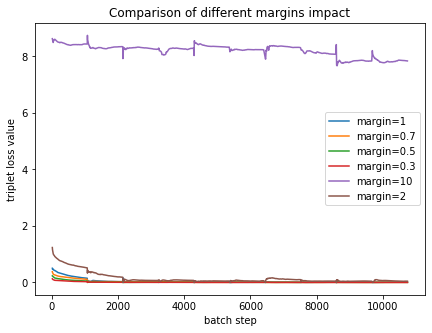
\includegraphics[width=.9\linewidth]{study-doc/experiment_margin/assets/margin_all_plot.png}
  \caption{triplet loss from all margins}
  \label{fig:sub-margin-all}
\end{subfigure}%
\begin{subfigure}{.5\linewidth}
  \centering
  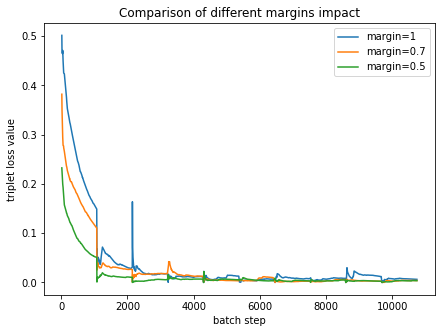
\includegraphics[width=.9\linewidth]{study-doc/experiment_margin/assets/margin_5_7_10_plot.png}
  \caption{triplet loss from margins=\texttt{0.5, 0.7, 1.0}}
  \label{fig:sub-margin-5-7-10}
\end{subfigure}
\caption{Plot of the triplet loss value of the margin experiment}
\label{fig:margin-experiment-triplet-loss-plot}
\end{figure}
\noindent
This experiment aims to show the affect of changing the margin $\alpha$ within a triplet loss on the DCASE dataset. A very important hyperparameter when training a triplet loss is the margin, denoted as $\alpha$. The margin makes sure that the network is not allowed to output the trivial solution, where all the embeddings vectors are zero or contain the same values. Within the triplet loss function, it is used to put a limit on how far the network can push the negative sample away to improve the loss. Thus the distance of the negative sample has to be higher than the distance from the anchor to the positive sample plus the margin $\alpha$. This experiment aims to show the importance of the margin as well as to find the optimal one for the DCASE dataset.
\newline
\newline
The hyperparameters used for this experiment are shown in the corresponding study doc in the appendix \ref{app:Study-Doc}. The margin is evaluated using a state of the art ResNet18 architecture on the DCASE dataset. The hyperparameters in section \textit{Feature representation} as well as the sample rate are the default ones proposed by the organisers of the DCASE challenge within the baseline project. The margin is evaluated for six different values \texttt{[0.3, 0.5, 0.7, 1, 2, 10]}.
\newline
\newline
Five models with the same hyperparameters, were trained for ten epochs. The value of the triplet loss is the most important criteria for selecting the optimal margin since the margin has the most significant impact on the loss function. Figure \ref{fig:sub-margin-all} shows all the trained models in a single plot to visualise the impact on changing the margin. From this figure, the resulting embeddings improved from the trivial solution as the margin is increased. Thus as the margin is decreased the total number of triplets generated whose loss is higher than zero decreases, therefore, they do not contribute to the training of the model thus reducing the accuracy of the outputted embedding’s.
\newline
\newline
There is a vast difference in the value of the loss values. The \texttt{margin=10} has by far the highest loss value of approximately 8, which is very intuitive since the distance to the opposite has to be higher than the distance to the neighbour plus the margin, which is in this case \texttt{8}. This constraint is tough to satisfy, and therefore the loss is relatively high.
\newline
\newline
The smallest loss value is the one from the \texttt{margin=0.3}. The reason for that is the same as for the high margin, but vice-versa. The constraint it has to satisfy is that the distance to the opposite has to be higher than the distance to the neighbour plus the margin. This is very easily satisfied since it is a relatively small distance.
\newline
\newline
The figure \ref{fig:sub-margin-5-7-10} shows the triplet loss of the margin values \texttt{0.5, 0.7, 1.0}. It can be seen that the loss is fairly similar and approaches zero.
\newline
\newline
Since the highest and lowest margin can be omitted simply by examining the triplet loss plot because the lowest margin does not contribute to the training and the highest sets a constraint which can only be satisfied in a small number of cases, in the other cases it is a much harder decision since the loss value is fairly the same. However, when looking at the resulting embedding space, it can be seen that the \texttt{margin=1.0} distances between the centroids of each label are fairly equally distributed, which is the optimal outcome. Figure \ref{fig:dist-margin-1} shows the distance matrix of the \texttt{margin=1.0}. Whereas the other margins do not have such an equally distributed distance matrix, which indicates that one or more label can be distinguished better than others. However, the optimal solution should be that the distances from all clusters are fairly the same. Therefore the \texttt{margin=1.0} is chosen as the optimal parameter for the DCASE dataset and is used in all of the further experiments as the standard hyperparameter.
\begin{figure}[tb]
\centering
    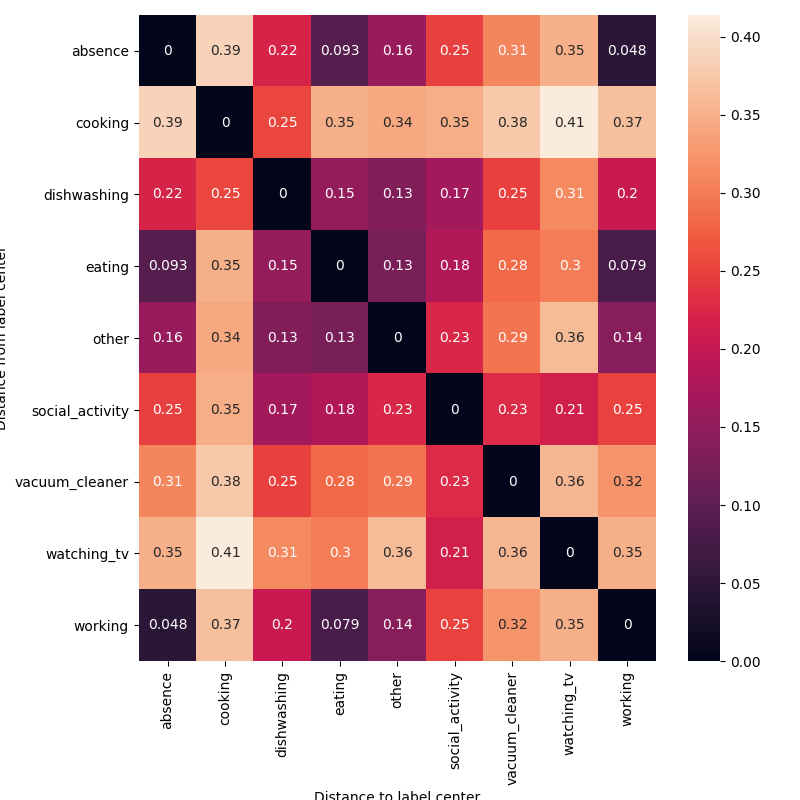
\includegraphics[width=0.5\linewidth]{study-doc/experiment_margin/assets/distance_mat_margin_1.png}
    \caption{Distance matrix of the margin=\texttt{1.0}}
    \label{fig:dist-margin-1}
\end{figure}

\subsection{Experiment: segment size}
\label{sub:Experiment-Segment-Size}
\begin{figure}[tb]
\centering
    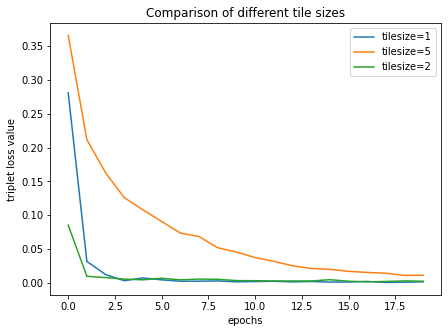
\includegraphics[width=0.5\linewidth]{study-doc/experiment_tile_size/assets/tile_sizes_plot.png}
    \caption{Plot of the triplet loss of the different tile sizes}
    \label{fig:tile-size-plot}
\end{figure}
\noindent
The experiment aims to show the effect of the size of the audio segments which is used as the size of the triplets. The size of each triplet, which is fed to the network, is an essential hyperparameter which needs to be carefully chosen. Because it specifies how much information each segment contains and is therefore fed to the network. If the segments are chosen too small, it does not contain enough information to distinguish between categories. If the size is too big, the segment contains too much information, and therefore, the model needs to work with a lot more data and gets a lot heavier. This experiment is conducted to search an optimal segment size for the triplets.
\newline
\newline
The hyperparameters used for this experiment are shown in the corresponding study doc in the appendix \ref{app:Study-Doc}. The experiment is conducted using a state of the art ResNet18 architecture on the DCASE dataset. The hyperparameters in section \textit{Feature representation} as well as the sample rate are the default ones proposed by the organisers of the DCASE challenge within the baseline project. The sample tile size is evaluated for three different values \texttt{[1, 2, 4]} in seconds.
\newline
\newline
Three models with the same hyperparameters were trained for 20 epochs. The value of the triplet loss is the primary evaluation criteria which is used to compare the different triplet sizes since it has the most effect on this value because it should show how much of an audio sample is needed to distinguish between different classes. Figure \ref{fig:tile-size-plot} shows all the trained models in a single plot to visualise the impact of changing the sample size. Nevertheless, it is quite hard to interpret the different graphs since all of them are near zero.
\newline
\newline
The figure \ref{fig:tile-size-plot} shows that the tile size 5s has the highest loss value while the tile sizes 1s and 2s have relatively similar values. However, this does not mean that the tile size of 5s is the worst out of the three, it instead means that the model finds it harder to distinguish audio files when a larger sample is available, which is pretty evident since longer samples contain more information.
\newline
\newline
The figure \ref{fig:tile-size-plot} further shows that the tile sizes of 1s and 2s have a very steep graph at the beginning and then hardly change their value. This indicates that it is relatively simple to achieve a good loss value with small audio samples, which means that the model can easily distinguish between small samples.
\newline
\newline
Both of these interpretations of the plot is pretty straight forward, but when the resulting embedding space is further examined using the Embedding Projector from the tensorboard, it can be seen that the tile size of 5s (\ref{fig:embedding-5s}) results in much clearer clusters than the tile size of 1s (\ref{fig:embedding-1s}). 
\newline
\newline
If the optimal parameter for the sample tile is only chosen from the loss value and therefore, from the plot \ref{fig:tile-size-plot}, it would be quite hard. However, since the visualisation of the embedding space shows a clear benefit in using a larger sample, the \textbf{sample tile size of 5s} is chosen to be the optimal one for the DCASE dataset. This can be explained because smaller samples much often contain sounds which do not indicate a specific sound in that class, say for example there is a two-second silence in a sound file of the class eating, it would be projected in the nearby region of silence in a sound of a different class, which is useful for other applications but since the goal is to achieve a best possible embedding space, this is not a satisfying result. Therefore, the larger sound segments are more robust to such problems, since they hold much more information about the resulting class. 
\newline
\newline
If the thesis focused on supervised triplet loss, it would make sense to cut the audio files in much smaller segments than in the unsupervised setting, since in supervised learning the triplet selection makes sure that the clustering focuses on the classes and not some other arbitrary criteria, which happens in unsupervised learning. In the unsupervised triplet loss, it is challenging to examine what exactly is being clustered, because there can be an underlying structure which can not be seen for us humans.
\begin{figure}[tb]
\centering
\begin{subfigure}{.5\linewidth}
  \centering
  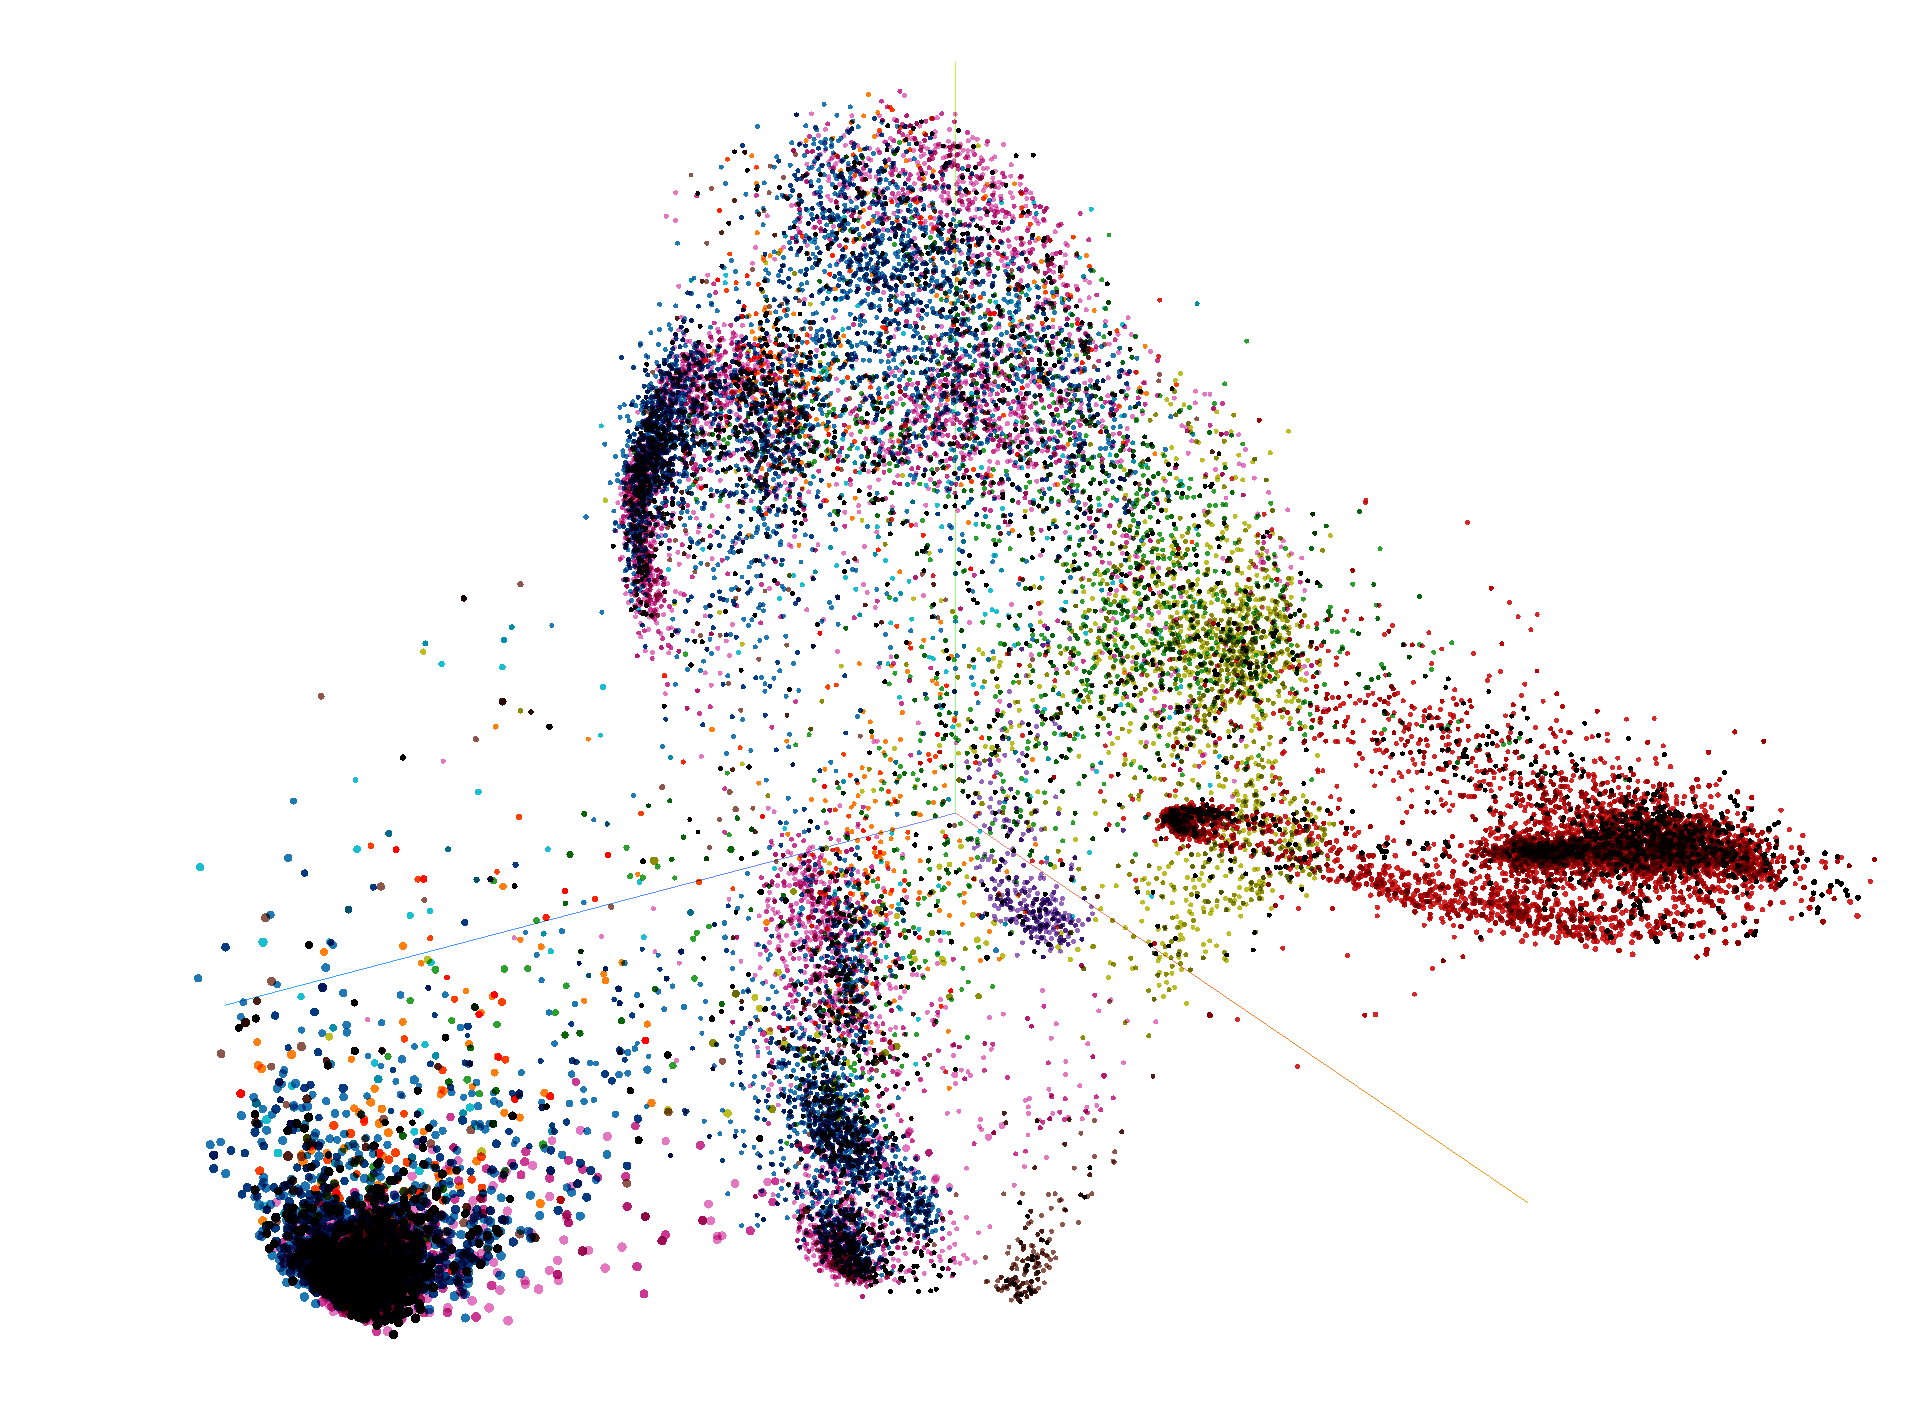
\includegraphics[width=.9\linewidth]{study-doc/experiment_tile_size/assets/embedding_space_5s.png}
  \caption{tile size 5s}
  \label{fig:embedding-5s}
\end{subfigure}%
\begin{subfigure}{.5\linewidth}
  \centering
  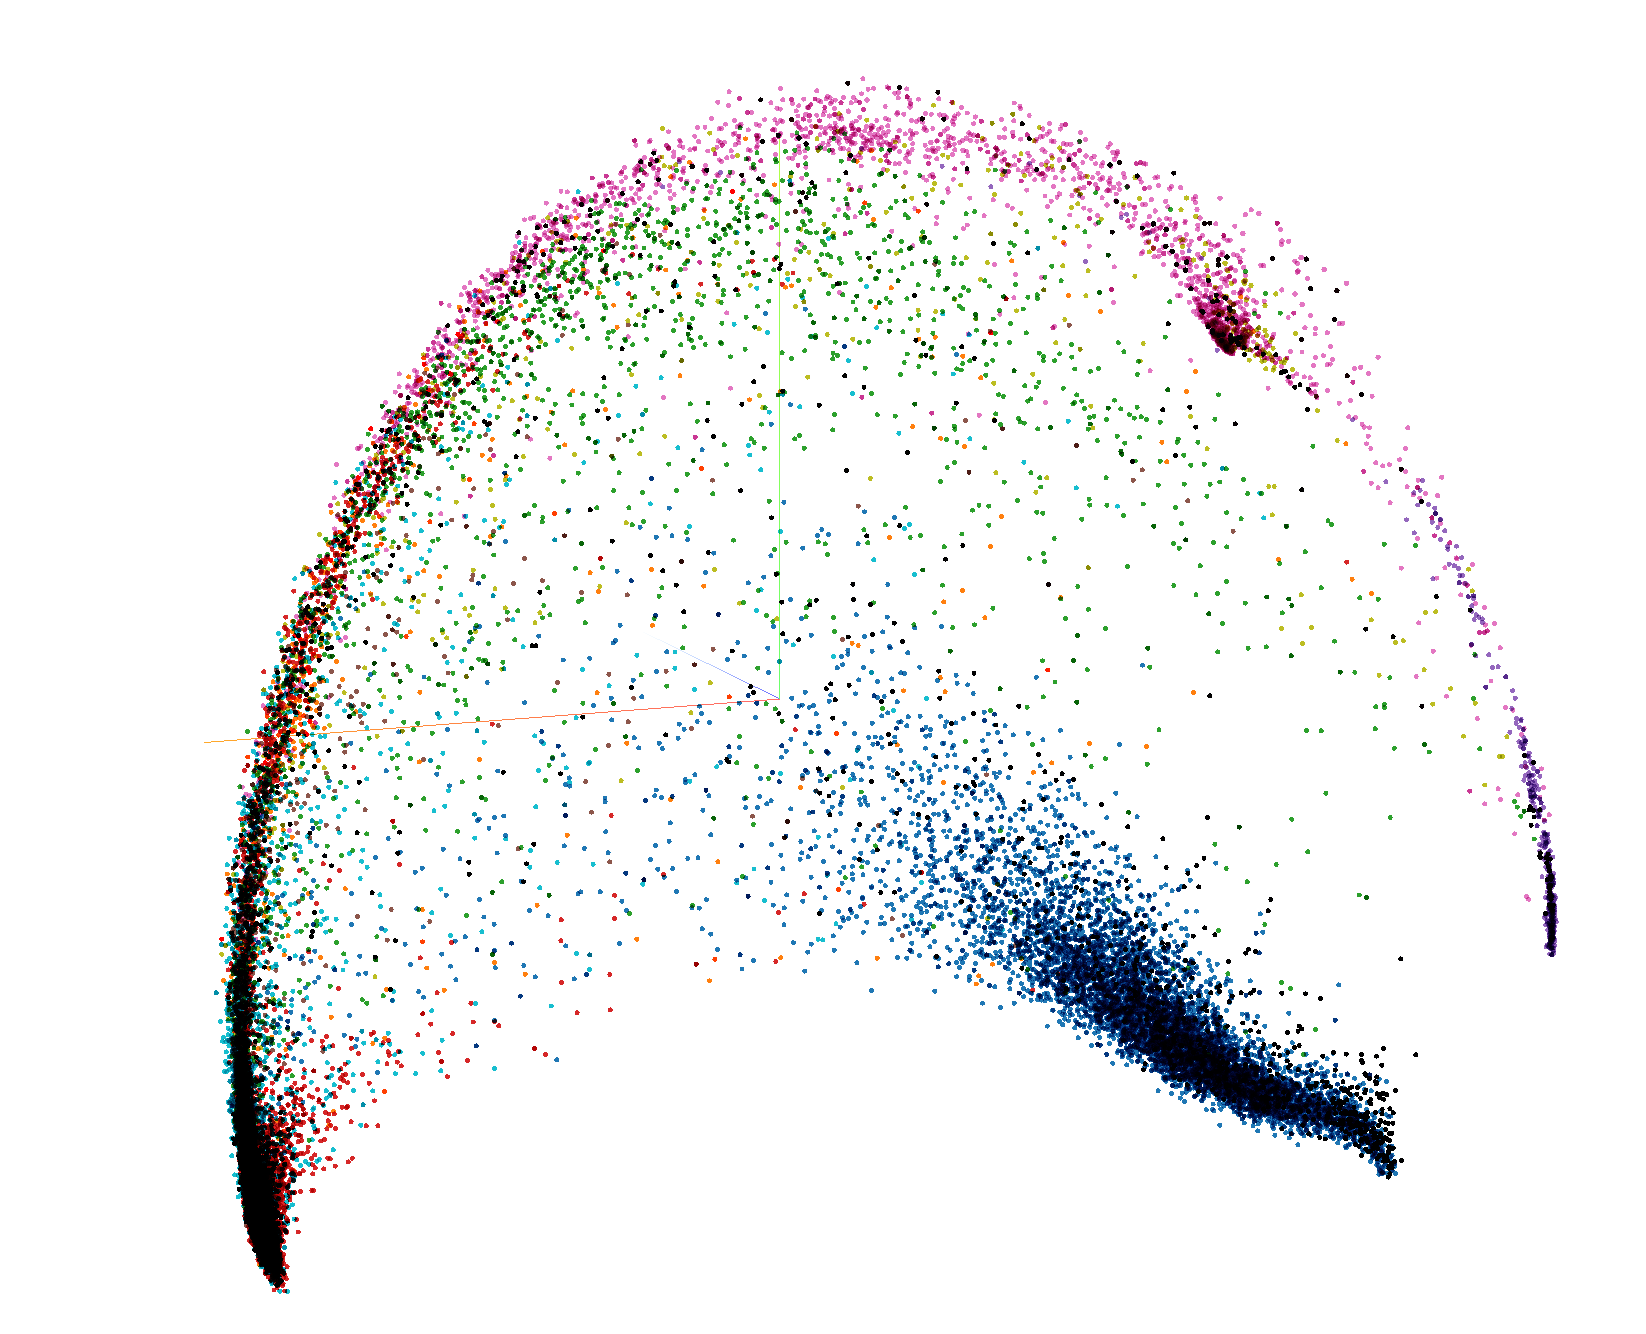
\includegraphics[width=.9\linewidth]{study-doc/experiment_tile_size/assets/embedding_space_1s.png}
  \caption{tile size 1s}
  \label{fig:embedding-1s}
\end{subfigure}
\caption{Visualisation of the embedding space from the tile size 5s and 1s}
\label{fig:tile-size-experiment-embedding-space}
\end{figure}

\subsection{Experiment: embedding size}
\begin{figure}[t]
\centering
    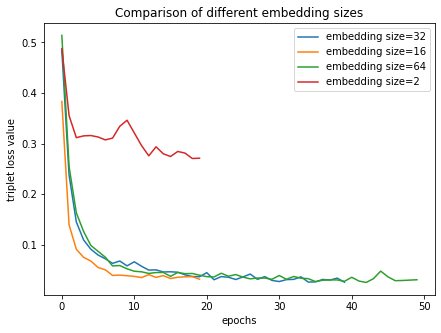
\includegraphics[width=0.5\linewidth]{study-doc/experiment_embedding_size/assets/plot_embedding_sizes.png}
    \caption{Plot of the triplet loss of the different embedding sizes}
    \label{fig:plot-embeddings-epochs}
\end{figure}
The experiment aims to show the effect of the size of the last dense layer from the embedding architecture, further called the \textbf{embedding size}. The size of the embedding space is essential for the performance, since choosing the wrong hyperparameter can lead to over- or underfitting of the model. The size defines how many dimensions the resulting embedding space has. Therefore if this parameter $e$ is selected to be too big, the model almost certainly overfits, because the model has many options to project the input data onto the embedding space. However, if $e$ is chosen to be too small, there is not enough room to project inputs in different regions. This experiment aims to search an optimal parameter for $e$.
\newline
\newline
The experiment is conducted using a state of the art ResNet18 architecture on the DCASE dataset. The hyperparameters in section \textit{Feature representation} as well as the sample rate are the default ones proposed by the organisers of the DCASE challenge within the baseline project. The embedding size $e$ is evaluated for four different values \texttt{[2, 16, 32, 64]}.
\newline
\newline
Four models with the same hyperparameters were trained for a different amount of epochs. The training was stopped when no more learning was observed. 
\newline
\newline
Comparing different embedding sizes is pretty hard since most of the metrics in the thesis focus on distances between embedding points. In higher dimensional embedding spaces, distances have a different scale and different meanings. This is especially true if small embedding sizes, such as \texttt{2}, and large sizes, such as \texttt{64}, are compared with each other. Therefore a simple classifier was trained on the resulting embedding spaces, and the metrics of the classifier was compared to find the optimal parameter. To further compare the embedding spaces, they were visualised using the Tensorboard Embedding Projector and manually compared with each other.
\newline
\newline
The figure \ref{fig:plot-embeddings-epochs} shows the different triplet loss values of the embedding sizes. The embedding size \texttt{2} has a significantly higher value than other embedding sizes, which shows that in the two-dimensional embedding space, it is a lot harder to project the data points apart from each other. Whereas in high dimensional embedding spaces, the model can easier build clusters.
\begin{figure}[t]
\centering
\begin{subfigure}{.33\linewidth}
  \centering
  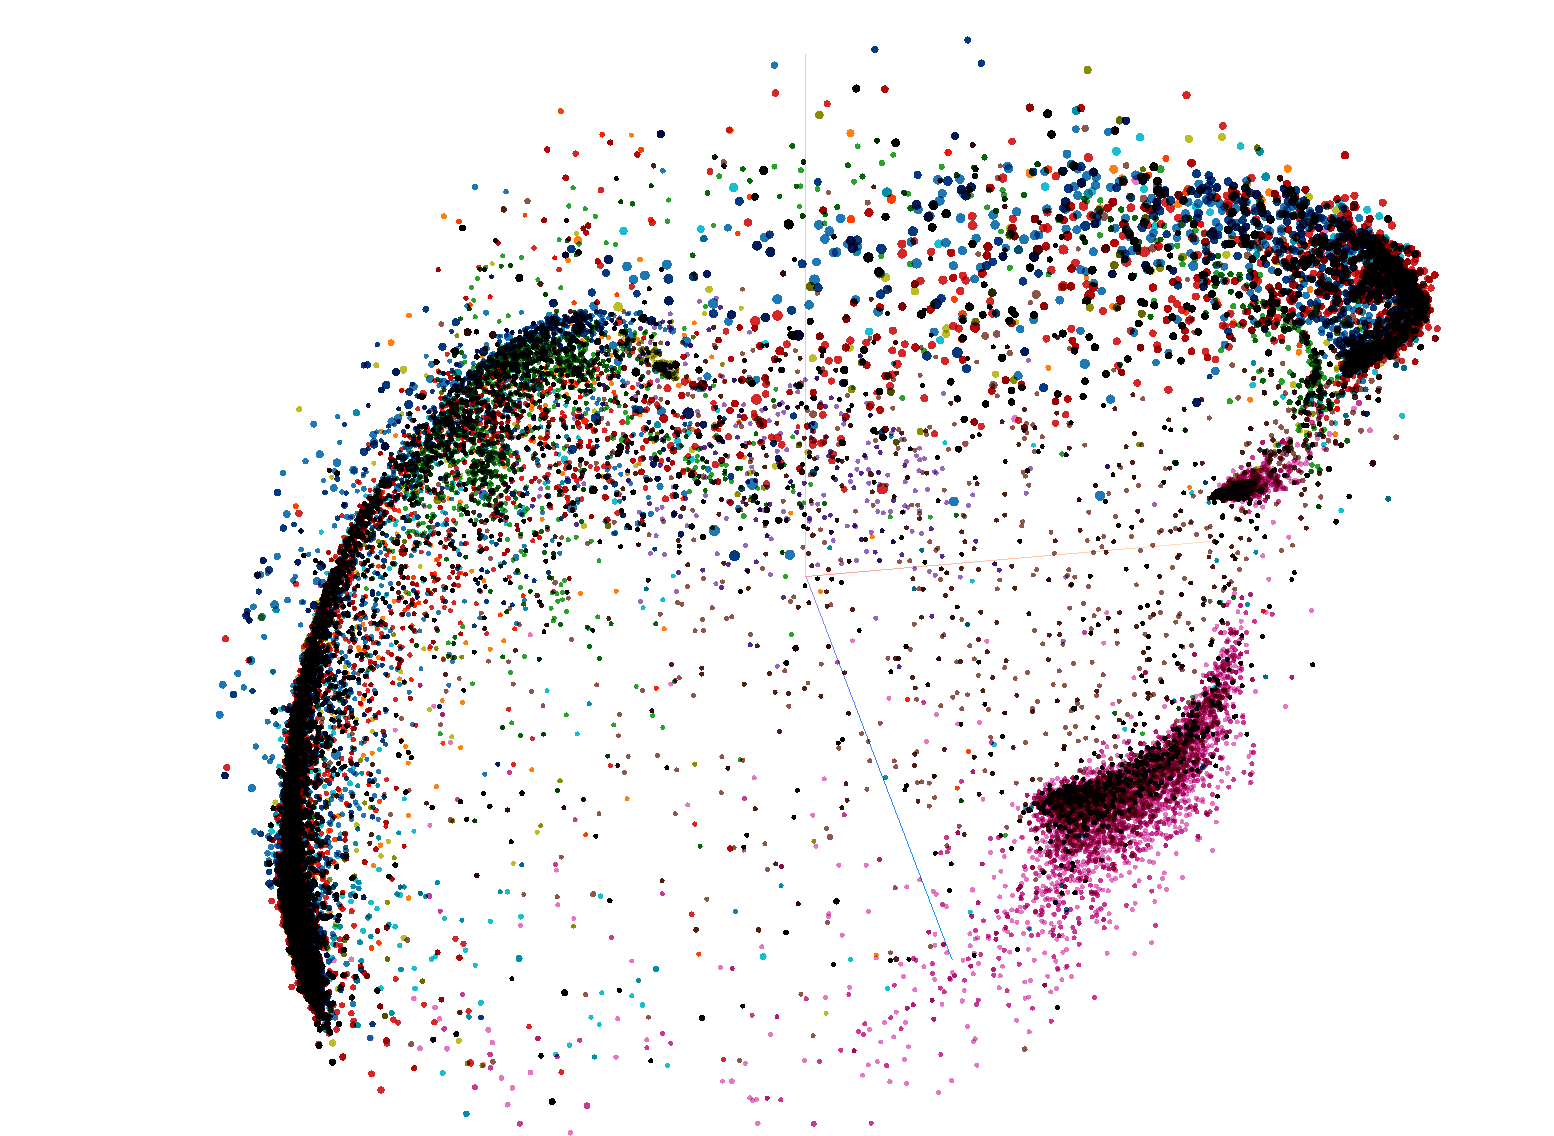
\includegraphics[width=.9\linewidth]{study-doc/experiment_embedding_size/assets/embedding_space_16.png}
  \caption{embedding size 16}
  \label{fig:embedding-space-16}
\end{subfigure}%
\begin{subfigure}{.33\linewidth}
  \centering
  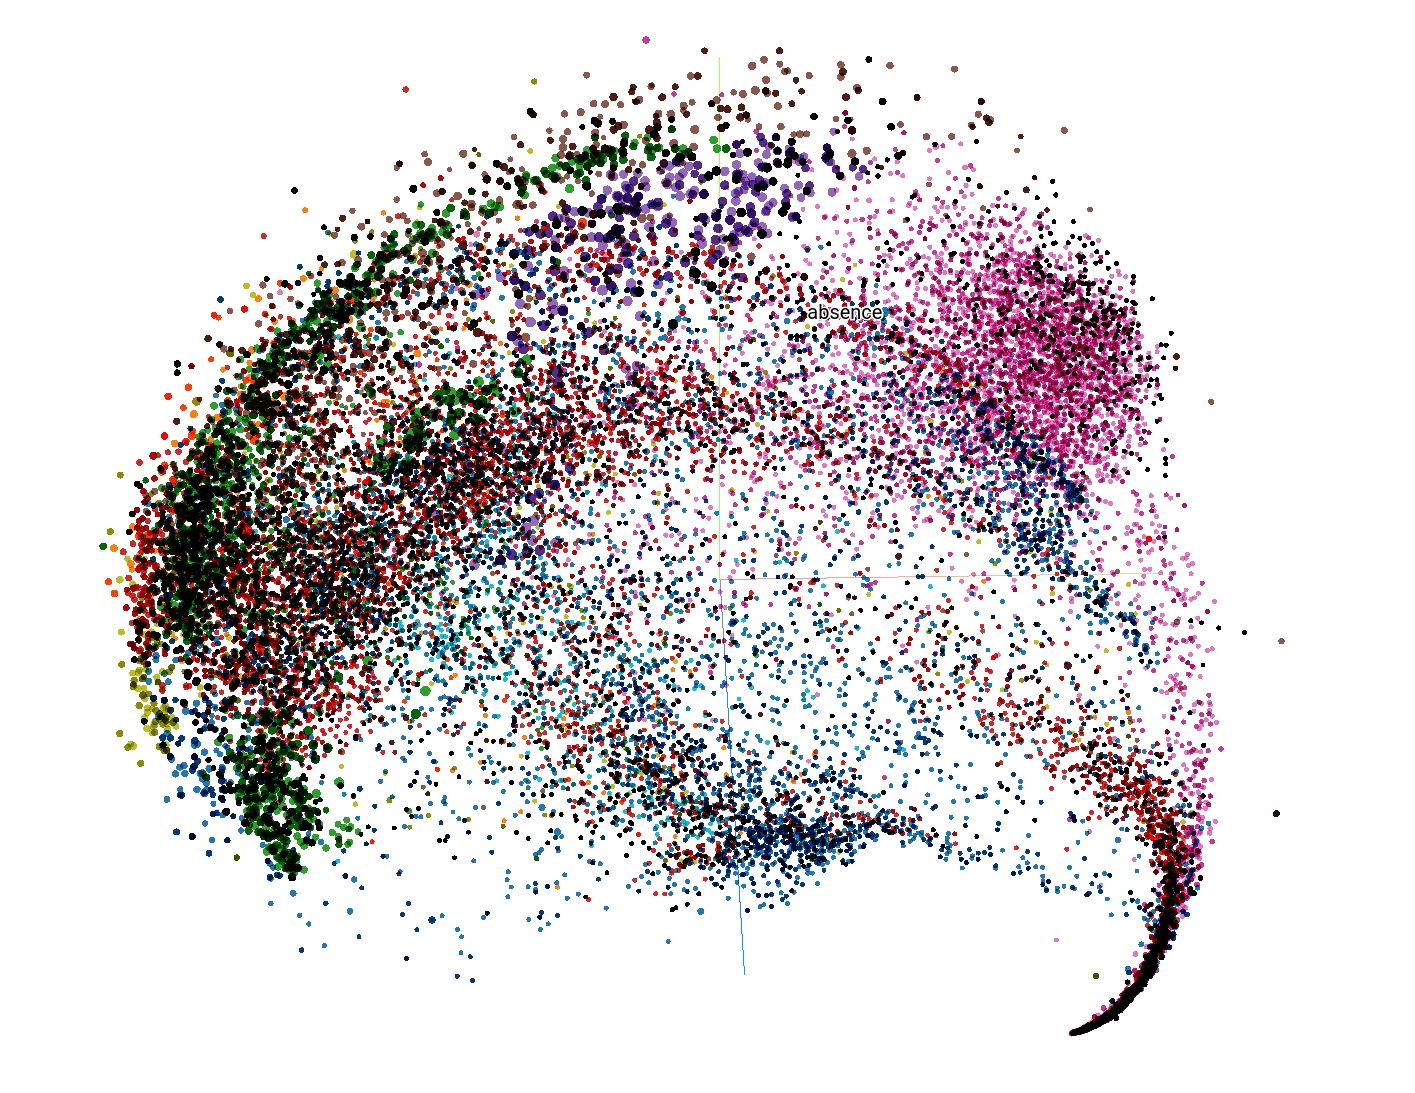
\includegraphics[width=.9\linewidth]{study-doc/experiment_embedding_size/assets/embedding_space_32.png}
  \caption{embedding size 32}
  \label{fig:embedding-space-32}
\end{subfigure}%
\begin{subfigure}{.33\linewidth}
  \centering
  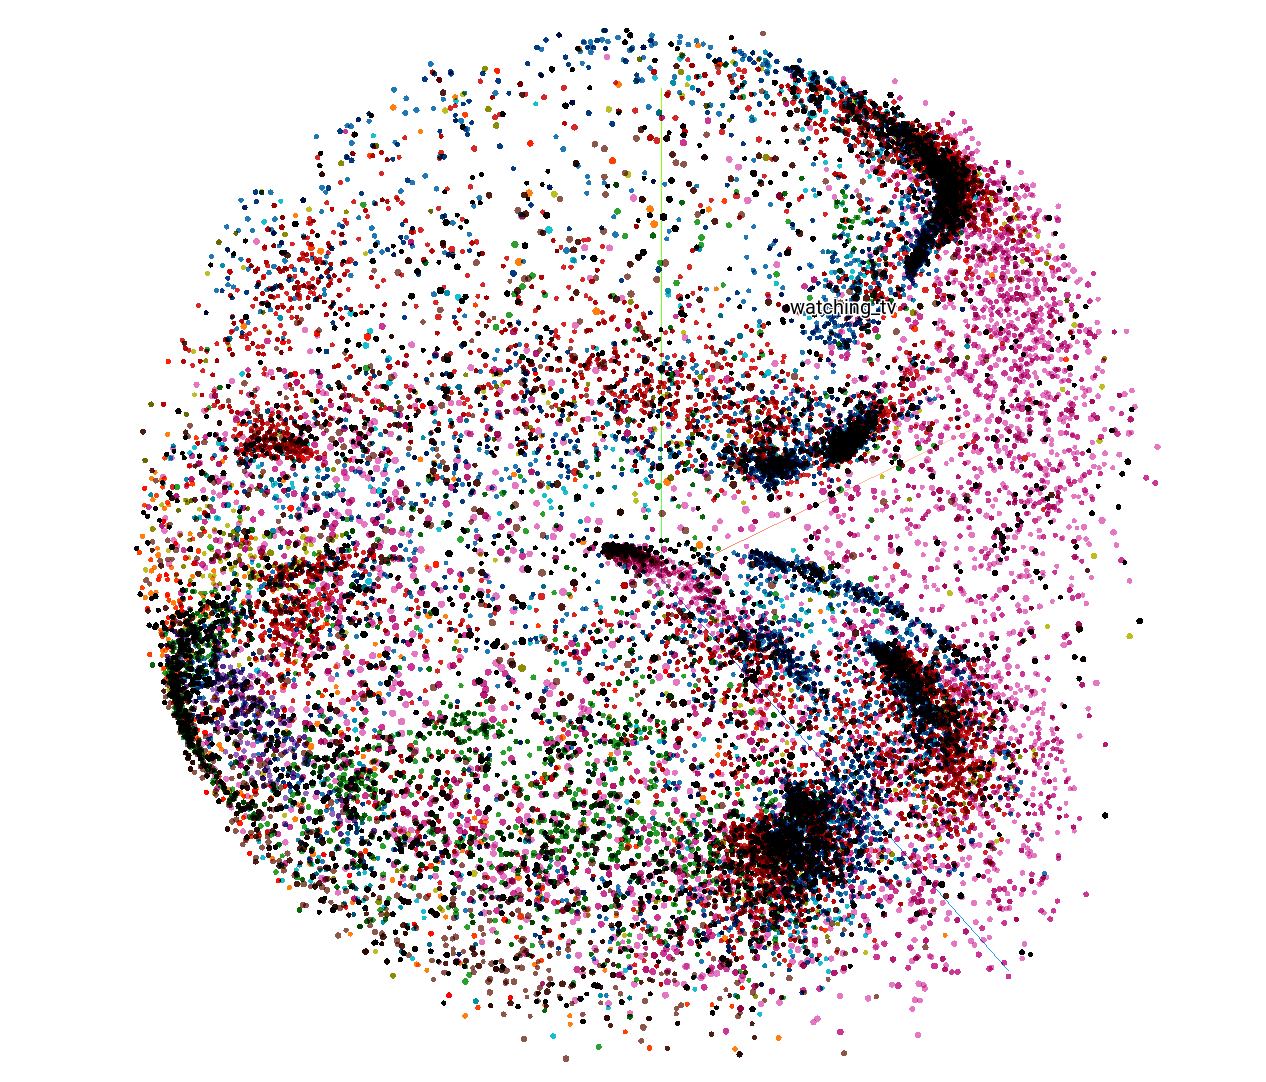
\includegraphics[width=.9\linewidth]{study-doc/experiment_embedding_size/assets/embedding_space_64.png}
  \caption{embedding size 64}
  \label{fig:embedding-space-64}
\end{subfigure}
\caption{Plot of the resulting embedding spaces}
\label{fig:embedding-size-experiment-embedding-space}
\end{figure}
\newline
\newline
\noindent
The plot further shows that the loss value of the embedding sizes \texttt{16, 32, 64} are relatively similar and are therefore further compared by examining their resulting embedding space. Which is shown in figure \ref{fig:embedding-space-16}, \ref{fig:embedding-space-32} and \ref{fig:embedding-space-64}. The result shows that there are vast differences in the embedding spaces, even though the triplet loss value is not that different. The embedding size of \texttt{16} shows only approximately four resulting clusters, which indicates a noisy embedding space where small classes are not well separated from each other. The embedding space of \texttt{32} and \texttt{64} show significant more resulting clusters and they result therefore in a better embedding space. However, it is to say that both embedding spaces further have more noise in it than the lower-dimensional space.
\newline
\newline
The graph \ref{fig:embedding-size-classifier-f1} shows the resulting F1 score when a simple logistic classifier is trained on top of the resulting embedding space. Since the DCASE dataset is heavily unbalanced, the F1 score is compared. All of the classifiers are trained for 20 epochs using the same parameters as the one for training the embedding space. The figure \ref{fig:embedding-size-classifier-f1} shows that the F1 score of the embedding space \texttt{16} is the highest out of the three.
\newline
\newline
The graph \ref{fig:embedding-size-classifier-loss} shows the sparse categorical cross-entropy loss value of the embedding spaces \texttt{16} and \texttt{64}.
\newline
\newline
The figure \ref{fig:plot-embeddings-epochs} shows that the smallest embedding size can be omitted since it has the highest triplet loss value significantly. The other three embedding spaces have quite similar values and are, therefore, further compared. The trained classifier on top of the embedding space shows (figure \ref{fig:embedding-size-classifier-f1}) that the embedding size \texttt{32} can be omitted since it has a significantly lower score than the others. The figure \ref{fig:embedding-size-classifier-f1} shows, that the embedding size \texttt{16} has achieved the highest F1 score of approximately \texttt{0.39}. However, the figure \ref{fig:embedding-size-classifier-loss} shows that the loss value of the embedding size \texttt{16} converges, which indicates that the training process is finished and the classifier will not show any improvements when training longer. The embedding size \texttt{64} has a lower F1 score, but the loss value is still decreasing at the end of epoch 20, which indicates that the model can benefit from further training. Further training will increase the F1 score until it converges.
\begin{figure}[t]
\captionsetup{format=plain}
\centering
\begin{subfigure}{.5\linewidth}
  \centering
  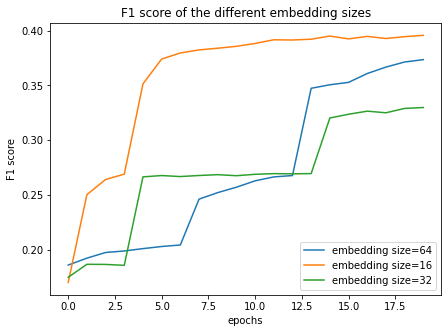
\includegraphics[width=.9\linewidth]{study-doc/experiment_embedding_size/assets/classifier_f1.png}
  \caption{F1 score}
  \label{fig:embedding-size-classifier-f1}
\end{subfigure}%
\begin{subfigure}{.5\linewidth}
  \centering
  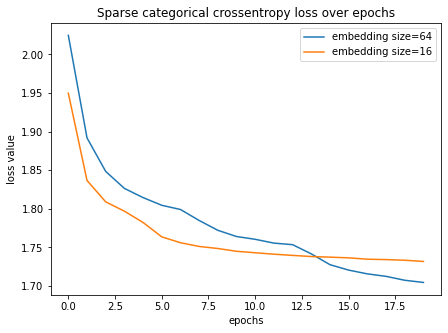
\includegraphics[width=.9\linewidth]{study-doc/experiment_embedding_size/assets/classifier_loss.png}
  \caption{sparse categorical cross-entropy loss}
  \label{fig:embedding-size-classifier-loss}
\end{subfigure}
\caption{graph of the metrics from the different classifiers trained on top of the resulting embedding spaces}
\label{fig:embedding-size-experiment-classifier-metrics}
\end{figure}
\newline
\newline
\noindent
Because of this result, the optimal embedding size, out of the four, is \texttt{64}, since it has an optimal triplet loss value, a high enough F1 score and the loss value still decreases after 20 epochs of training the classifier.
\newline
\newline
This experiment showed that changing the dimension of the embedding space results in significant different embedding spaces and therefore resulting clusters. The experiment should further be conducted for the music dataset because this parameter highly depends on the underlying structure of the data. 
\newline
\newline
For the next experiments, the embedding space size \texttt{64} is chosen. The embedding space should also be evaluated on significant higher spaces, such as \texttt{256} or \texttt{512}.
\newline
\newline
The experiment further showed another important conclusion, that the longer the embedding space is trained, the more the loss value oscillates which indicates that a learning rate decay should be used to reduce the learning rate over time (\ref{fig:plot-triplet-64}).
\begin{figure}[h]
\centering
    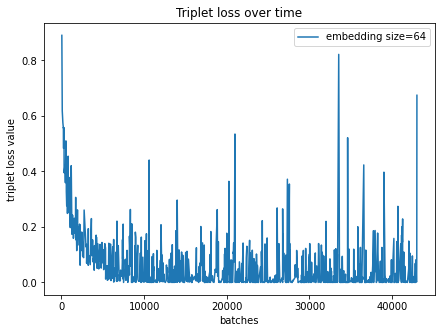
\includegraphics[width=0.5\linewidth]{study-doc/experiment_embedding_size/assets/plot_triplet_loss.png}
    \caption{Plot of the triplet loss of the embedding space 64}
    \label{fig:plot-triplet-64}
\end{figure}

\subsection{Experiment: regularisation factor}
\begin{figure}[ht]
\centering
    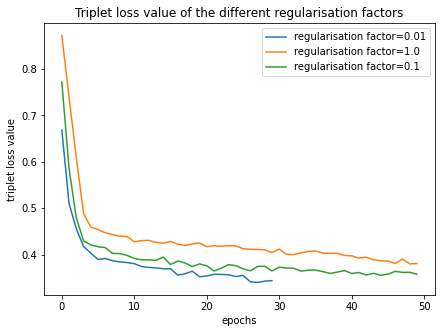
\includegraphics[width=0.5\linewidth]{study-doc/experiment_regularisation/assets/triplet_loss.png}
    \caption{Plot of the triplet loss values of the different regularisation factors $\lambda$}
    \label{fig:plot-triplet-loss}
\end{figure}
\noindent
The experiment aims to show how the embedding space will change for different regularisation factors. The purpose of regularisation is that it prevents models from overfitting, by penalising high weights. The regularisation is calculated for all layers weights separately and is then added to the standard loss function, in this case, the triplet loss. The combined loss value is then used to calculate the gradients and update the weights of the model. There are a lot of different regularisation techniques, which successfully reduce the chance of overfitting. In this experiment, the \texttt{L2-Regularisation} is used and evaluated with different values. The parameter which will control the value of the \texttt{L2-Regularisation} is denoted as $\lambda$.
\newline
\newline
The experiment will be conducted using a state of the art ResNet18 architecture on the DCASE dataset. The hyperparameters in section \textit{Feature representation} as well as the sample rate are the default ones proposed by the organisers of the DCASE challenge within the baseline project. The regularisation factor $\lambda$ will be evaluated for three different values \texttt{[1.0, 0.1, 0.01]}.
\newline
\newline
Comparing the effect of different regularisation factors on the embedding space is pretty hard, since comparing embedding spaces is not very straight forward and is a rather tricky task. This is mainly because of the fact, that to visualise the high dimensional embedding space in a way humans can perceive it, it has to be reduced to two or three dimensions. Therefore the original space can not be examined, and the visual representation is always an approximation of the space in a lower dimension. To still compare the embedding spaces and the effect of $\lambda$, a simple logistic classifier is trained on top of the resulting embedding spaces, which aims to show how well a simple classifier works with the embedding space. This will show how good the resulting embedding space is. The classifier is trained for 20 epochs with the same parameters as the embedding model.
\newline
\newline
Figure \ref{fig:plot-triplet-loss} shows the difference between the triplet loss values of the embedding model when changing the regularisation factor. It shows that the model with $\lambda = 1.0$ has the highest triplet loss value, which is obvious, since the bigger the regularisation factor is, the longer the model optimises the weights to satisfy the constraint of having very small weights. The lower $\lambda$, the faster the model optimises the triplet loss value. $\lambda = 0.01$ has the lowest triplet loss value.
\begin{figure}[tb]
\captionsetup{format=plain}
\centering
\begin{subfigure}{.5\linewidth}
  \centering
  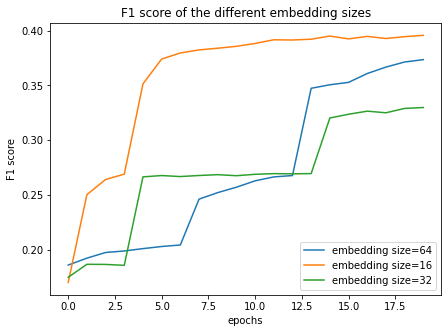
\includegraphics[width=.9\linewidth]{study-doc/experiment_embedding_size/assets/classifier_f1.png}
  \caption{F1 score}
  \label{fig:regularisation-experiment-classifier-f1}
\end{subfigure}%
\begin{subfigure}{.5\linewidth}
  \centering
  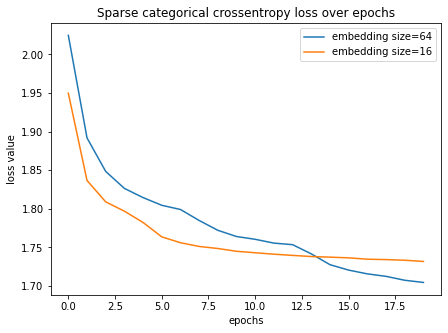
\includegraphics[width=.9\linewidth]{study-doc/experiment_embedding_size/assets/classifier_loss.png}
  \caption{sparse categorical cross-entropy loss}
  \label{fig:regularisation-experiment-classifier-loss}
\end{subfigure}
\caption{graph of the F1 score and the loss from the different classifiers trained on top of the resulting embedding spaces}
\label{fig:regularisation-experiment-classifier-metrics}
\end{figure}
\newline
\newline
\noindent
Figure \ref{fig:regularisation-experiment-classifier-f1} shows the different F1 scores of the logistic classifier, which is trained on top of the embedding architecture. This provides an idea of how well the embedding space separates the classes and therefore gives a performance gain. The figure \ref{fig:regularisation-experiment-classifier-f1} shows, that the regularisation factor $\lambda = 0.01$ has the highest F1 score. This result is significant since this particular embedding space was only trained for 30 epochs, unlike the other models, who are trained for 50. 
\newline
\newline
The figure \ref{fig:regularisation-experiment-classifier-loss} shows the corresponding categorical cross-entropy loss values of the trained classifiers. It shows that the loss of $\lambda = 1.0$ converges before $\lambda = 0.1$ or $\lambda = 0.01$. The figure further shows, that the loss values of $\lambda = 0.1$ and $\lambda = 0.01$ are not converged and would benefit from a longer training.
\newline
\newline
Figure \ref{fig:regularisation-experiment-classifier-f1} shows that the highest regularisation factor $\lambda = 1.0$ can be omitted since it did not accomplish an equally good F1 score. This result is expectable since a high regularisation factor forces the embedding model to work with very small weights and can, therefore, lead to performance loss. 
\newline
\newline
The regularisation factor $\lambda = 0.1$ and $\lambda = 0.01$ only show very little difference in F1 performance as well as in triplet loss value. Never the less, the factor $\lambda = 0.01$ provides slightly better results than $\lambda = 0.1$. 
\newline
\newline
The triplet loss value and the loss value of the classifier of the regularisation factor $\lambda = 0.01$ is still decreasing at the end of the training, which indicates that the model can benefit from further training. Further training will increase the resulting embedding space and the F1 score of the classifier until it converges.
\newline
\newline
The figure \ref{fig:plot-triplet-loss} and \ref{fig:regularisation-experiment-classifier-f1} further indicate one very important conclusion, that the value of the triplet loss is directly related to how well the classifier performs, which is further an indication how well the created embedding space works. Therefore the assumption is, that the lower the triplet loss value, the better the classifier performs and the better the embedding space is. 
\newline
\newline
The experiment shows that the regularisation factor $\lambda = 0.01$ gives the best results out of the three since it has an optimal triplet loss value, a high enough F1 score and the loss value still decreases after 20 epochs of training the classifier.
\newline
\newline
The experiment showed that the regularisation factor $\lambda$ has an essential impact on the embedding space and should therefore not be chosen to be too big nor too small since this either leads to over- or underfitting. The optimal regularisation parameter $\lambda$ should be further examined in later and more extensive experiments with a lot more values for $\lambda$.

\subsection{Experiment: feature representation}
\begin{figure}[htb]
\captionsetup{format=plain}
\centering
\begin{subfigure}{.5\linewidth}
  \centering
  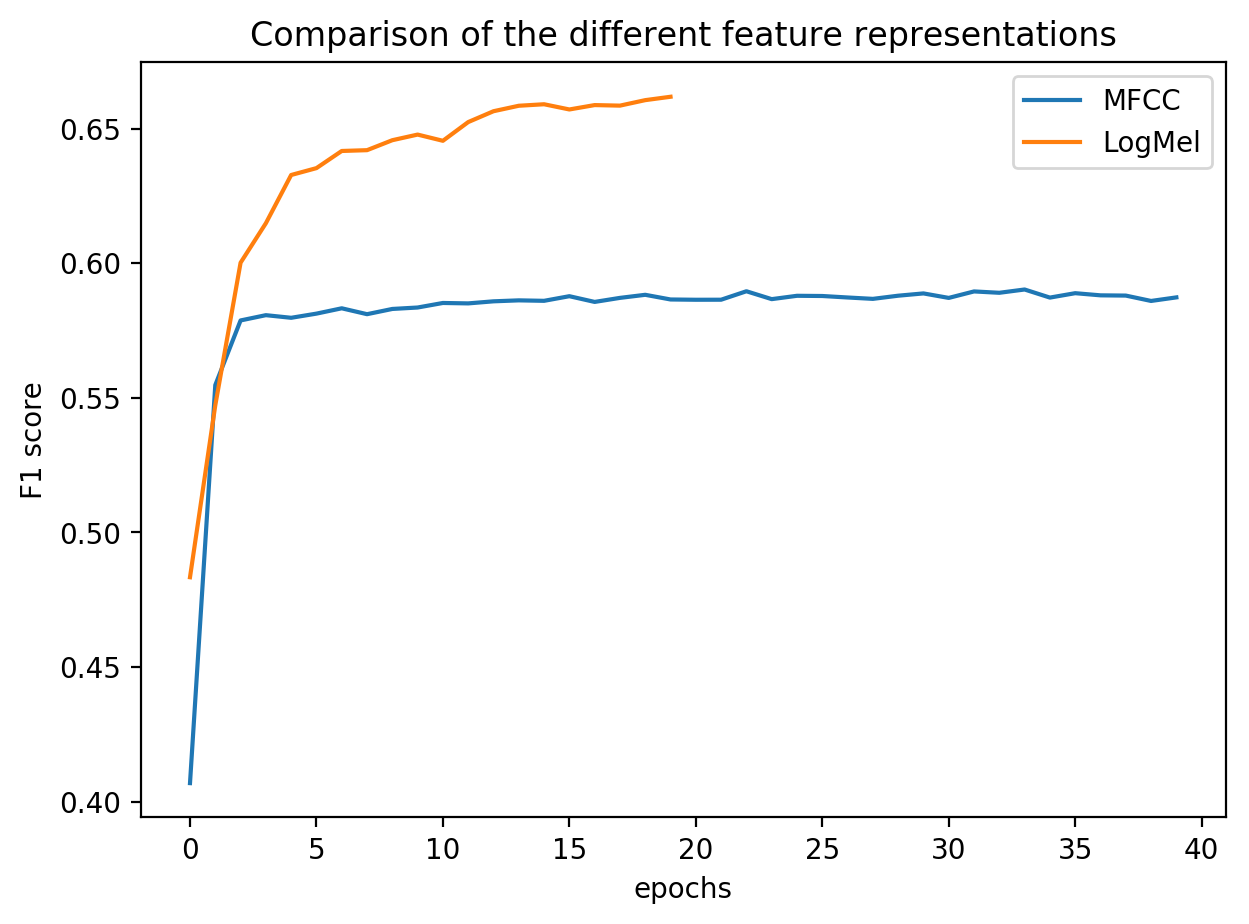
\includegraphics[width=.9\linewidth]{study-doc/experiment_feature/assets/f1_feature_representation.png}
  \caption{Triplet loss}
  \label{fig:plot-triplet-loss-feature-representations}
\end{subfigure}%
\begin{subfigure}{.5\linewidth}
  \centering
  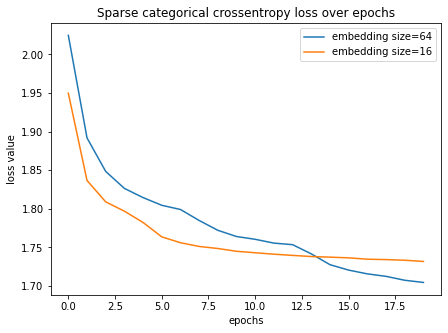
\includegraphics[width=.9\linewidth]{study-doc/experiment_embedding_size/assets/classifier_loss.png}
  \caption{F1 score of the classifier}
  \label{fig:classifier-f1-feature-represenations}
\end{subfigure}
\caption{Plot of the metrics from the models trained using the different feature representations}
\label{fig:feature-experiment-metrics}
\end{figure}
\noindent
The purpose of the feature representation is to represent the audio in a more compact form than the raw audio. The feature representation further determines the input size for the model. There are a lot of different ways to represent the an audio file in a more compact form. One of the most popular representations is the MFCCs, which is heavily used in the audio domain. However in the recent years, the trend leads more towards using the log Mel spectrogram, which is very similar to the MFCCs, but by omitting the last step of the calculation. This experiment aims to find the optimal feature representation for the thesis.
\newline
\newline
The experiment will be conducted using a state of the art ResNet18 architecture on the DCASE dataset. The hyperparameters in section \textit{Feature representation} as well as the sample rate are the default ones proposed by the organisers of the DCASE challenge within the baseline project.
The optimal feature representation will be evaluated for \texttt{[LogMel, MFCCs]}.
\newline
\newline
Comparing the effect of different regularisation factors on the embedding space is pretty hard, since comparing embedding spaces is not very straight forward and is a rather tricky task. This is mainly because of the fact, that to visualise the high dimensional embedding space in a way humans can perceive it, it has to be reduced to two or three dimensions. Therefore the original space can not be examined, and the visual representation is always an approximation of the space in a lower dimension. To still compare the feature representations, a simple logistic classifier is trained on top of the resulting embedding spaces, which aims to show how well a simple classifier works with the embedding space. This will show how good the resulting embedding space is. The classifier is trained for 40 epochs with the same parameters as the embedding model.
\newline
\newline
Figure \ref{fig:plot-triplet-loss-feature-representations} shows the difference between the triplet loss from the model using the different feature representations. It shows that the model trained using the MFCCs results in a significantly lower loss than the model using the log Mel spectrogram. The model using the log Mel spectrogram seem already converging at epoch 30.
\newline
\newline
Figure \ref{fig:classifier-f1-feature-represenations} shows the different F1 scores of the logistic classifier, which is trained using the embedding space as input. This provides an idea of how well the embedding space separates the classes and therefore gives a performance gain. The figure \ref{fig:classifier-f1-feature-represenations} shows clearly that the classifier trained on top of the log Mel spectrogram reached a higher F1 score. The metric further shows, that the classifier using the MFCCs embedding space fails to improve the F1 score over time, whereas the classifier for the log Mel spectrogram shows a definite increase over time.
\newline
\newline
From figure \ref{fig:plot-triplet-loss-feature-representations} it seems that the optimal feature representation is the MFCCs since it reached a significantly lower loss value. It further shows that the model would be able to benefit from further training since the model is still decreasing. However, when looking at the resulting F1 score of the classifiers (figure \ref{fig:classifier-f1-feature-represenations}), the result shows, that even though the MFCCs representation reached a lower triplet loss, the classifier fails to separate the resulting clusters using a hyperplane. 
\newline
\newline
This experiment shows that the optimal feature representation for the current thesis is using the log Mel spectrogram, since it resulted in a higher F1 score of the classifier, even though the triplet loss value is higher than the one using the MFCCs. 
\newline
\newline
This is mainly due to the different nature of the feature representations. The MFCCs representation input size (498, 13) is significantly lower than the log Mel spectrogram representation input size (498, 128). The MFCCs is a more compact representation, which seems to have a negative effect on the model performance.
\newline
\newline
This experiment shows that the model benefits from using a representation which has more features and therefore, the log Mel spectrogram is used as the optimal representation for the thesis.

\subsection{Triplet loss}
\label{sub:Results-Triplet-Loss}
The first experiments were conducted using the standard triplet loss equation given by \ref{eq:Triplet-Loss}. The loss value is given by calculating the triplet loss for the entire batch of triplets and afterwards taking the mean of the batch of triplet losses. This resulted in the triplet loss value, which was used to optimise the model. After a few experiments, one could identify that the triplet loss value decreased rapidly to almost zero and then only oscillated minimally. A low loss value typically means that the model is performing well, and the weights of the network only need to be changed slightly, and therefore the training is almost finished. However, it was observed that this was not true for the trained models since there was still much noise in the embedding space. This indicated that the loss value did not represent the actual performance of the model accurately.
\newline
\newline
In order to solve this problem, the calculation of the loss was further examined. This showed that after the first few epochs of training, many triplets did already satisfy the equation \ref{eq:Triplet-Loss}. However, this is a normal behaviour when training an unsupervised triplet loss, since the triplet selection is purely based on assumptions and not facts like it is for supervised triplet loss. When using assumptions, there is a high possibility, that the triplets are easily satisfied and therefore classify as easy triplets. It would be optimal always to select the hardest neighbour as well as selecting the hardest opposite for each anchor segment. However, this is not feasible and is, therefore neglected.
\newline
\newline
When calculating the triplet loss of a batch of triplets where 70\% of the batch satisfy the triplet loss constraint, the batch of triplet losses contains 70\% zeros. Afterwards, when taking the mean of the batch, the resulting loss value is really low, only because it consists of many zeros. Therefore the loss function is optimised to filter the zero values and only to calculate the mean of the non-zero loss values. This results in a significantly higher loss value, even in later epochs. The equation \ref{eq:Triplet-loss-justification} shows the difference between the ordinary and the mean filtered loss value, for illustration purposes, a batch size of 10 is taken.
\myequations{Justification behind triplet loss changes}
\begin{equation}
    \centering
    \begin{gathered}
        \text{triplet loss with mean:}\\
        \mathcal{L} = \frac{0 + 0+ 0+ 0+ 0+ 0+ 0+ 0.3+ 0.6+ 0.8}{10} = 0.17 \\
        \\
        \text{triplet loss with mean filtering:}\\
        \mathcal{L} = \frac{0+ 0+ 0+ 0+ 0+ 0+ 0+ 0.3+ 0.6+ 0.8}{3} = 0.56
    \end{gathered}
    \label{eq:Triplet-loss-justification}
\end{equation}
Two embedding models were trained using the same hyperparameters for 40 epochs, to test the newly proposed triplet loss calculation. The only difference is the calculation of the triplet loss. After the training has finished, a logistic classifier was trained for 20 epochs using the resulted embedding space. Both classifiers were then compared with each other, using the F1 score. This comparison is shown in figure \ref{fig:Triplet-Loss-Techniques}. There is a significant difference between the resulting scores, which indicates that the optimisation proposed above provided a significant benefit in comparison to the triplet loss without filtering. This notable difference is mainly because when training a model with mean filtering, the loss value remains a lot higher than without it, which results in better optimisation of the model. The mean filtering triplet loss is therefore used for all the experiments, because it provided a significant benefit.
\begin{figure}[ht]
\centering
    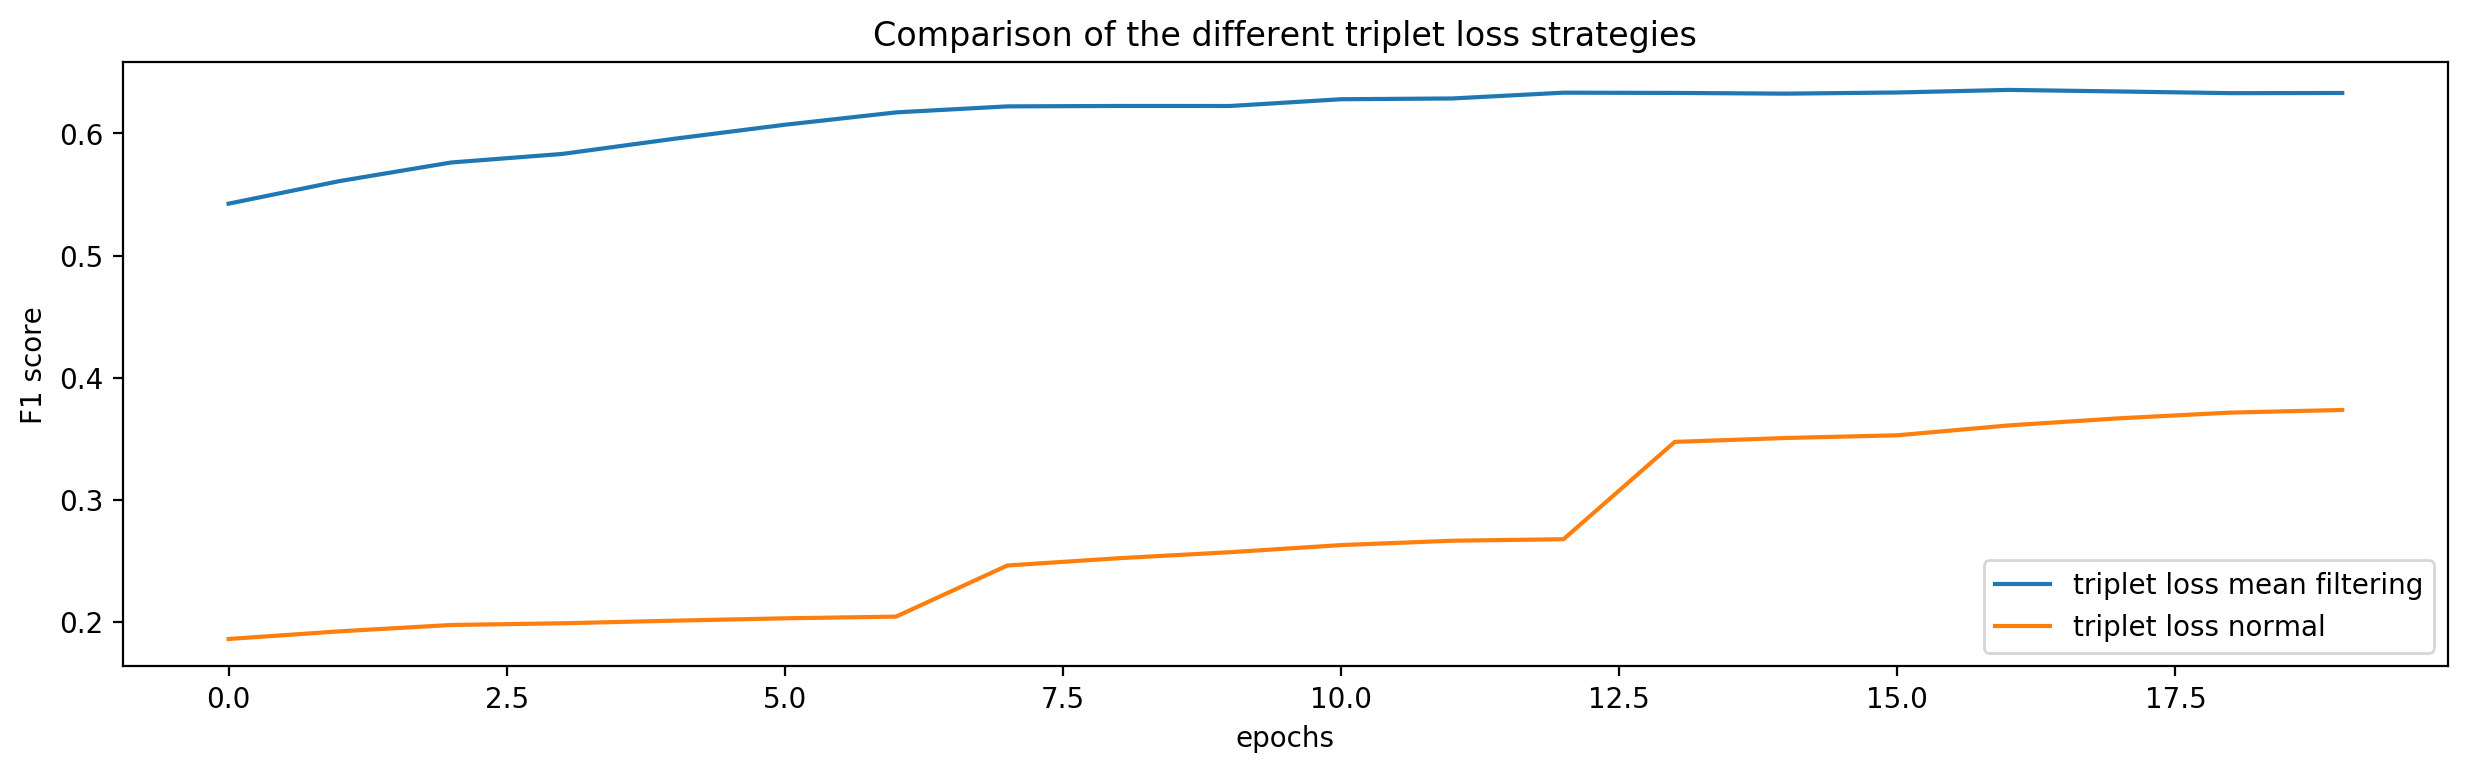
\includegraphics[width=0.6\linewidth]{img/Triplet-Loss-Comparison-Techniques.png}
    \caption{Triplet loss comparison of different techniques}
    \label{fig:Triplet-Loss-Techniques}
\end{figure}

\subsection{Resulting model}
\label{sub:Results-DCASE-Resulting-Model}
\begin{table}[ht]
    \captionsetup{format=plain}
    \centering
    \caption{Hyperparameters of the optimal embedding architecture for the noise detection dataset}
	\label{tab:Hyperparameters-DCASE}
    \begin{tabular}{l|l}
        \toprule
        \textbf{Hyperparameter} & \textbf{value} \\ 
        \midrule[1pt]
        Model & ResNet18 \\ 
        \hline
        Epochs & 110 \\ 
        \hline
        Batch size & 64 \\ 
        \hline
        Optimizer & Adam \\ 
        \hline
        Learning rate & 1e-5 \\
        \hline
        Margin & 1.0 \\
        \hline
        L2 regularisation amount & 0.01 \\
        \hline
        Embedding dimension & 256 \\
        \midrule[1pt]
        \multicolumn{2}{l}{\textit{Audio sample}} \\
        \midrule[1pt]
        Sample rate & 16000 \\ 
        \hline
        Sample tile size & 5s \\
        \hline
        Sample tile range & 5s \\
        \hline
        Convert to mono & True \\
        \midrule[1pt]
        \multicolumn{2}{l}{\textit{Feature representation}} \\
        \midrule[1pt]
        Feature extractor & LogMelExtractor \\ 
        \hline
        Input size & 498 x 128 \\
        \bottomrule
    \end{tabular}
\end{table}
\begin{figure}[ht]
\centering
    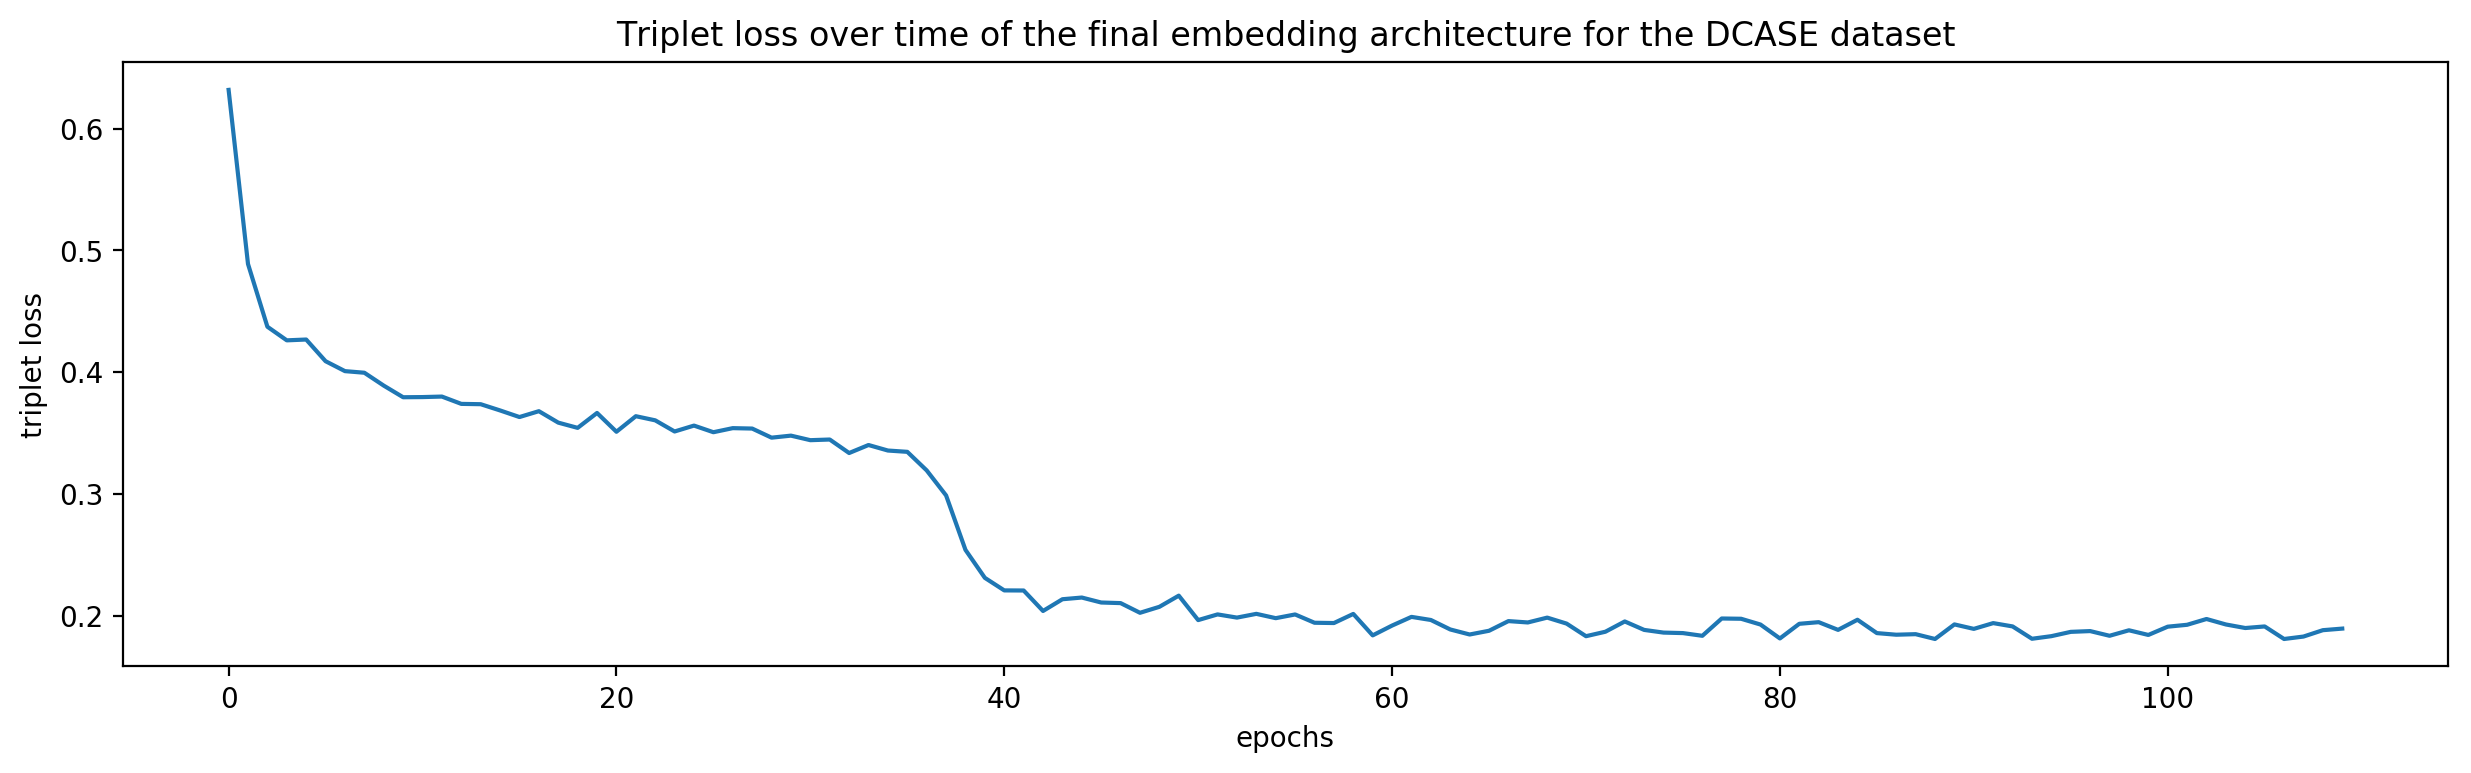
\includegraphics[width=0.6\linewidth]{img/Triplet_loss_DCASE_final.png}
    \caption{Triplet loss plot of the final embedding model for the noise detection dataset}
    \label{fig:Triplet-Loss-DCASE}
\end{figure}
The optimal embedding space architecture for the DCASE task 5 challenge in this thesis is given by the hyperparameters in table \ref{tab:Hyperparameters-DCASE} as well as in table \ref{tab:Hyperparameters-Detailed-DCASE}, which shows the hyperparameters in more detail.
\newline
\newline
The model was trained for 110 epochs and reached a triplet loss value of 0.1879, which is by far the lowest loss of all the different experiments. The triplet loss value is shown in figure \ref{fig:Triplet-Loss-DCASE}. The plot shows that the model has decreased a significant amount between the 34 and the 39 epoch. 

\subsection{Embedding space}
\label{sub:Eval-Embedding-Space-DCASE}
The embedding space was further examined to get detailed insights about the resulting clusters and the distances between them.  The entire development dataset was projected onto the embedding space and saved, including with the corresponding label, name and segment, to examine the embedding space. Afterwards the embedding space was converted into an \texttt{cKDTree} from \texttt{scipy}, which is a kd-tree for quick nearest-neighbor lookup. This tree was used to get the neighbours from a specific data point in the embedding space.
\newline
\newline
First, the miss-classified embeddings were further examined, this is done by looping over the entire embedding space and checking if the label of the selected embedding and 20 of its neighbours are all different. If that is so, the segment and its neighbours are further examined. The examination showed that most of the segments which belong to a different cluster as their label, consisted of a big part of silence or were purely silence, and were therefore projected to the region of silence. Most of these segments consisted of a part of silence, and after for example, seven seconds a sound was observed. However, when segmenting each audio in segments, there is a high possibility, that the segment only consists of silence. This shows that the embedding space clusters the segments by their meaning and not by their activity, which means that silence when performing, for example, the activity \textit{working} or \textit{eating}, will be projected in the near-by region. It was also observed that there are a lot of audios, which do not contain any sound and are therefore purely silence but have the label \textit{working}. These audio files should be examined further because there is a chance that they are miss-classified and should be assigned to the label \textit{absence}. However, it can be reasoned, that silence when performing the activity \textit{working} belongs to the activity, since there is a high possibility that the person does not make any sound but the model should still recognise this activity as \textit{working}. Nevertheless, this provided useful insights into the dataset as well as the embedding space. It was also observed that there are some audios, where a microphone malfunction is present and because of that are wrong classified, for example audio \texttt{DevNode3\_ex53\_42}.
\newline
\newline
The other examination of the embedding space focused on the correct classified segments and aimed to show the nature of the embedding space. The idea is to select two labels of the dataset, for example, \textit{working} and \textit{eating}, then to loop over the dataset and checking if the embedding belongs to one of these classes and further has five neighbours from the same label. If this is the case, the embedding will be appended to a list of the corresponding label. These lists are then used to calculate the mean of the clusters from each label. The checking of the neighbourhood of each embedding is used to neglect the problem of outliers in clusters. Afterwards, the distance between the clusters is calculated and divided by a specified number of steps, which indicates how many steps have to be taken to reach the other label. Then the centroid of the first label is taken, and the step difference is added to it. From this position, the nearest neighbours are taken and displayed. This process is repeated until the position of the other centroid label is reached. This \flqq walk through the embedding space\frqq can then be represented as an image (\ref{fig:Walk-through-DCASE}) or as a continuous recording of the segments appended with each other. This representation shows that the embedding space represents much meaning because when walking through the space, for example from \textit{working} to \textit{social\_activity} the figure \ref{fig:Walk-through-DCASE} shows that there is more sound activity when approaching \textit{social\_activity}. However this increase is done in a rather slow matter and for example in the figure \ref{fig:Walk-through-DCASE}, the line three represents audios from \textit{social\_activity} where there is still a lot of silence or quiet talking.
\begin{figure}[ht]
\captionsetup{format=plain}
\centering
    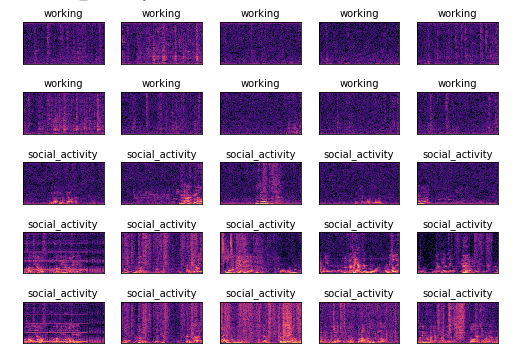
\includegraphics[width=0.8\linewidth]{img/Walk_through_dcase_space.png}
    \caption{\flqq walk through the embedding space\frqq \ of the DCASE space from \textit{working} to \textit{social\_activity}}
    \label{fig:Walk-through-DCASE}
\end{figure}

\subsection{Comparison to challenge results}
\label{sub:Eval-Comparison-DCASE}
One of the primary evaluations for the embedding space is how well a simple logistic classifier, which is trained on top of the embedding space, performs. The metrics of the classifier are used to compare and evaluate different embedding spaces and also to compare how well it performs in comparison to the models submitted in the DCASE task 5 challenge. The submitted architectures were compared using the F1 score of the evaluation dataset using. The main goal of the challenge was to show that models are able to recognise daily activities using different microphone arrays. Therefore, to compare the models in the challenge, the F1 score was calculated from the evaluation set where the microphones were unknown and were not present in the training dataset. The winner of the challenge was a team from IBM, which accomplished an F1 score on the unknown microphones of 88.4\% and a 90.4\% F1 score on the entire evaluation dataset. The embedding space in this thesis was only compared using the full evaluation dataset.
\newline
\newline
On the final embedding architecture for this challenge, described in \ref{sub:Eval-Embedding-Space-DCASE}, the trained classifier accomplished a macro-averaged F1 score of 62.19\% on the full evaluation dataset. The difference between the results of this thesis and the challenge is approximately 30\% to the winner and 20\% to the others. A detailed classification report is given by figure \ref{fig:classification-report-DCASE}, which shows the precision, recall and F1-score of each class. It can be seen that the classes \textit{other} and \textit{eating} are the hardest to classify. This is mainly due to the nature of their sounds and the high imbalance in the dataset. The class \textit{other} is used when an activity is performed, which does not belong to a label in the dataset and therefore contains a lot of different sounds. The label \textit{eating} is very hard to differentiate, because the sound of eating itself is very similar to \textit{dish washing} or \textit{cooking} since there are mainly noises of kitchen utilities present.
\begin{figure}[ht]
\captionsetup{format=plain}
\centering
    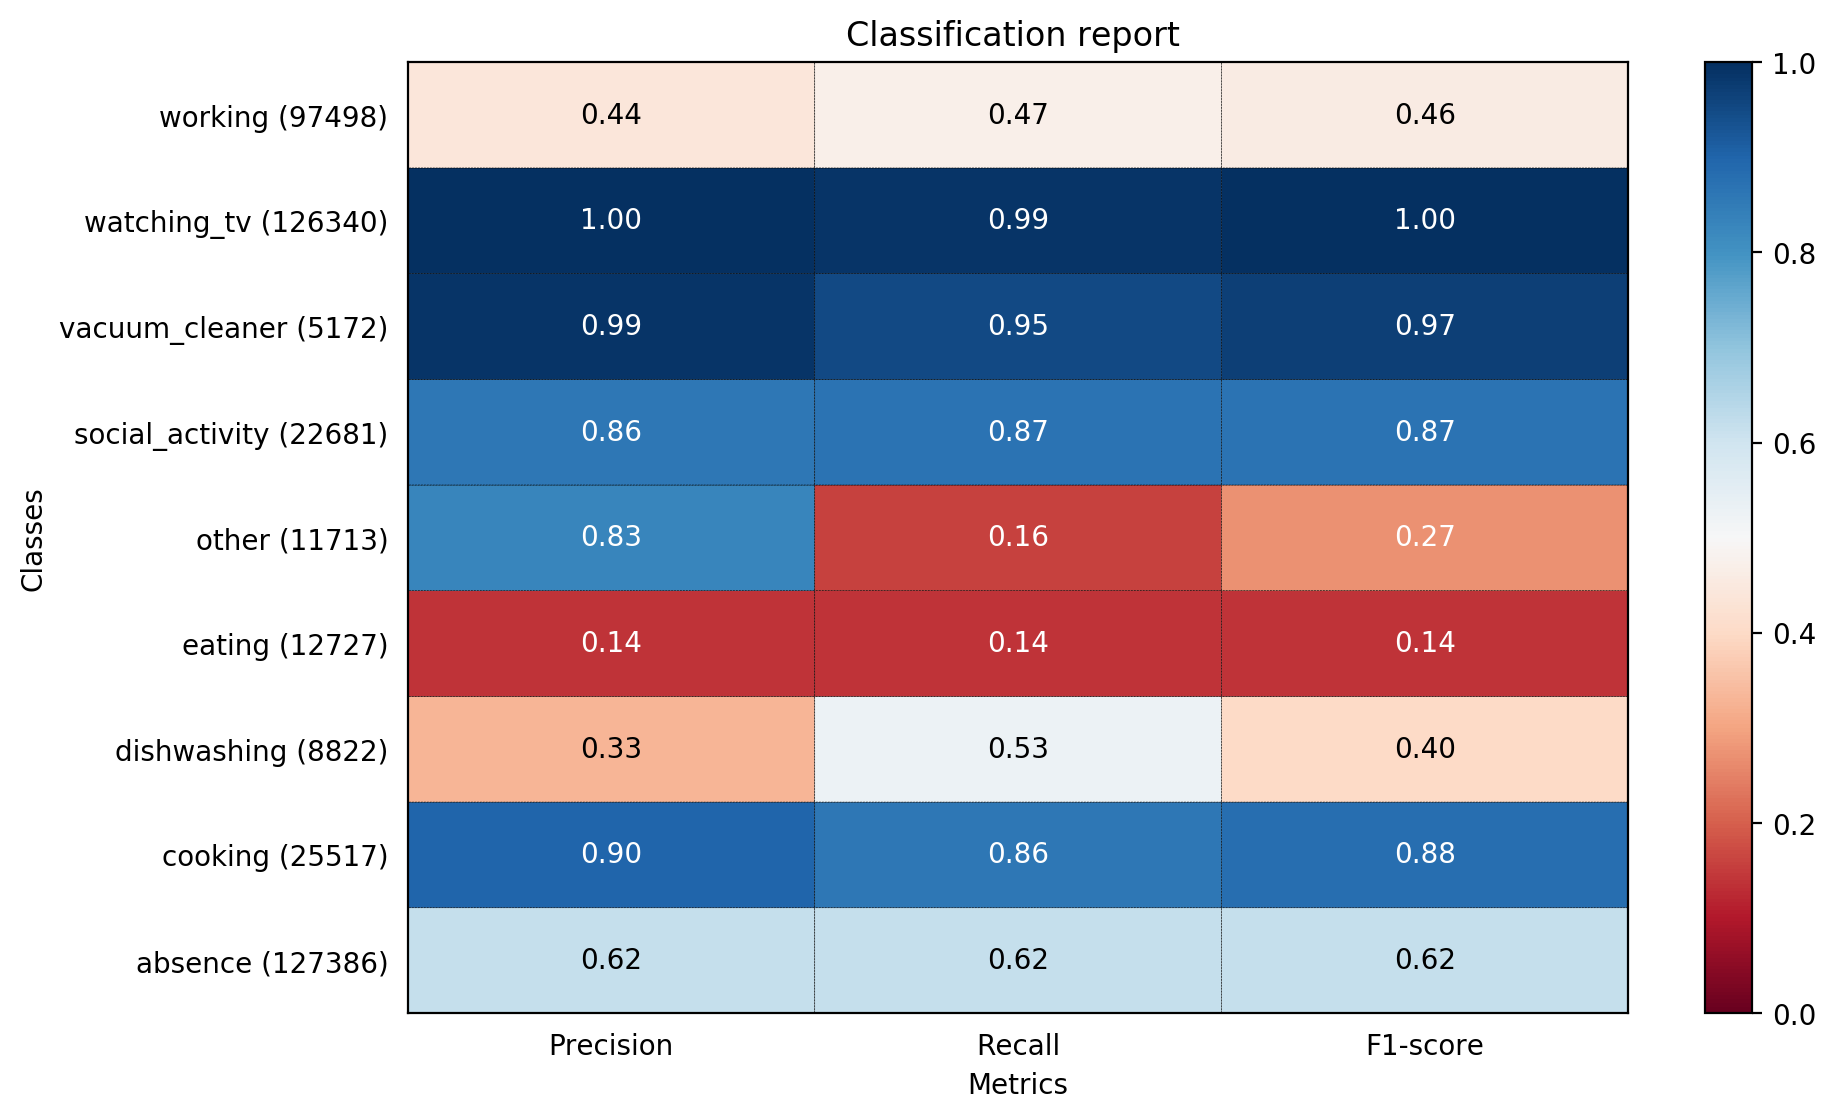
\includegraphics[width=0.8\linewidth]{img/DCASE_F1_classification_report.png}
    \caption{Classification report of the classifier on the evaluation dataset from the DCASE challenge}
    \label{fig:classification-report-DCASE}
\end{figure}

\subsection{Conclusion}
\label{sub:Eval-Conclusion-DCASE}
The results from the examination of the embedding space for the DCASE challenge are quite astonishing since the embedding space represents much meaning, such as the distribution of the clusters and miss-classified segments are off place. It is fascinating that all of this meaning can be extracted purely based on the nature of the sound rather than the underlying label. One of the most astonishing properties of the embedding space is that it can find miss-classified audios or even microphone malfunctions within the dataset. 
\newline
\newline
However, when comparing the model to the challenge results, the embedding space performs not so well, which means that there is a 20\% gap between the trained embedding model and the challenge results. Nevertheless, since the goal was not to beat the participants in the challenge, but rather to create an embedding space which represents meaning and the comparison to the challenge was only used to show the difference between the approaches, the accomplished results compared to the challenge are still good. Furthermore, if a more extensive architecture, such as a ResNet, would be trained on top of the embedding space, the results could be profoundly improved.
\newline
\newline
The resulting embedding model uses a state-of-the-art ResNet18 architecture, which resulted in good results. More massive architectures such as ResNet50 or ResNet152 were not evaluated due to the lack of time and resources. Other approaches, such as \gls{CRNN}, should also be evaluated to find the optimal state-of-the-art architecture. There is a possibility that using more massive architectures would result in a better embedding space since there are more weights available. However, the possibility of overfitting also increases. Nevertheless, experiments have to show how the embedding space varies when increasing the architecture and if there is a performance gain when doing so.

\section{Music dataset}
\label{sec:Results-Music}
This section describes the results of the experiments with the music dataset (\ref{sub:Music-Dataset}). The intention was to show that the created embedding space is applicable not only to the noise detection domain but can be used throughout the audio domain. The intention of using the embedding space was the same as for the \gls{DCASE} challenge dataset, to create an embedding space where distances represent the similarity between segments. When using the music dataset, this similarity between sound segments can then be used to find similar segments or to cluster segments by similarity. This section shows the examination of the embedding space to test if the model succeeded finding similarities, by first examining the embedding space manually (\ref{sub:Results-Music-Embedding-Space}), then by applying a clustering (\ref{sub:Results-Music-Clustering}) and then finally by conducting a qualitative analysis in the form of an interview with mister Emanuel Oehri (\ref{sub:Results-Music-Qualitative-analysis}). The final part of this section is to provide a conclusion about the model performance on the music dataset (\ref{sub:Results-Music-Conclusion}).

\subsection{Resulting model}
\label{sub:Results-Music-Resulting-Model}
\begin{table}[ht]
    \centering
    \caption{Hyperparameters of the optimal embedding architecture for the music dataset}
	\label{tab:Hyperparameters-Music}
    \begin{tabular}{l|l}
        \toprule
        \textbf{Hyperparameter} & \textbf{value} \\ 
        \midrule[1pt]
        Model & ResNet18 \\ 
        \hline
        Epochs & 130 \\ 
        \hline
        Batch size & 32 \\ 
        \hline
        Optimizer & Adam \\ 
        \hline
        Learning rate & 1e-5 \\
        \hline
        Margin & 1.0 \\
        \hline
        L2 regularisation amount & 0.01 \\
        \hline
        Embedding dimension & 256 \\
        \midrule[1pt]
        \multicolumn{2}{l}{\textit{Audio sample}} \\
        \midrule[1pt]
        Sample rate & 44100 \\ 
        \hline
        Sample tile size & 10s \\
        \hline
        Sample tile range & 40s \\
        \hline
        Convert to mono & True \\
        \midrule[1pt]
        \multicolumn{2}{l}{\textit{Feature representation}} \\
        \midrule[1pt]
        Feature extractor & LogMelExtractor \\ 
        \hline
        Input size & 998 x 128 \\
        \bottomrule
    \end{tabular}
\end{table}
The same embedding architecture as the one for the noise detection dataset, with mostly the same hyperparameters, was used. The hyperparameters for the music dataset are given by table \ref{tab:Hyperparameters-Music} and table \ref{app:detailed-hyperparameters-music}, which shows the hyperparameters in more detail. The difference in the hyperparameters is mainly due to the different structure of the dataset and their audio samples. In the \gls{DCASE} challenge dataset, the samples are already split into 10s segments, whereas the samples in the music dataset are full songs of a specific genre, which leads to variable audio lengths in the dataset. However, this does not make any difference in the input pipeline but instead gives an additional possibility to split the samples into larger segments. The experiment with the different segment sizes (\ref{sub:Experiment-Segment-Size}), showed that using larger segments results in much clearer clusters and therefore, in a better embedding space. Therefore the segment size was increased from 5s to 10s, which further resulted in a two times larger input size. This further led to the decrease of the batch size to 32, because of the initial batch size led to an out of memory exception due to the lack of larger computational resources. The increase of the neighbouring range is as well because there is the possibility of doing so due to the nature of the samples of the dataset. The increase provides a vaster possibility of triplet combinations, which the model can only profit from.
\newline
\newline
The resulting model was trained for 130 epochs, which took around seven and a half days, the training took this long, mainly because the triplet selection ant therefore also the splitting of the song was done on the fly in the input pipeline. The training process could be significantly decreased when using \texttt{TFRecords}\footnote{\href{https://www.tensorflow.org/tutorials/load\_data/tfrecord\#tfrecord\_files\_using\_tfdata}{www.tensorflow.org/tutorials/load\_data/tfrecord}}. However the conversion of the dataset to \texttt{TFRecords} was neglected since this would provide a more static dataset, rather than a more dynamic one. If the dataset is more dynamic, the model learns to handle differences in the dataset a lot better, since the dataset is continually changing and therefore focuses more on the underlying structure of each segment. However, this leads to models which need to be trained a lot longer than with a more static dataset.
\newline
\newline
The figure \ref{fig:Triplet-Loss-Music} shows the graph of the triplet loss value of the trained epochs. It shows that the model starts with a relatively high loss value and decreases over time. At the end of the training, at epoch 130, the model reached a triplet loss value of approximately 0.35. The graph further shows that the model could potentially profit from additional training with a lower learning rate to get an even lower triplet loss value.
\begin{figure}[ht]
\centering
    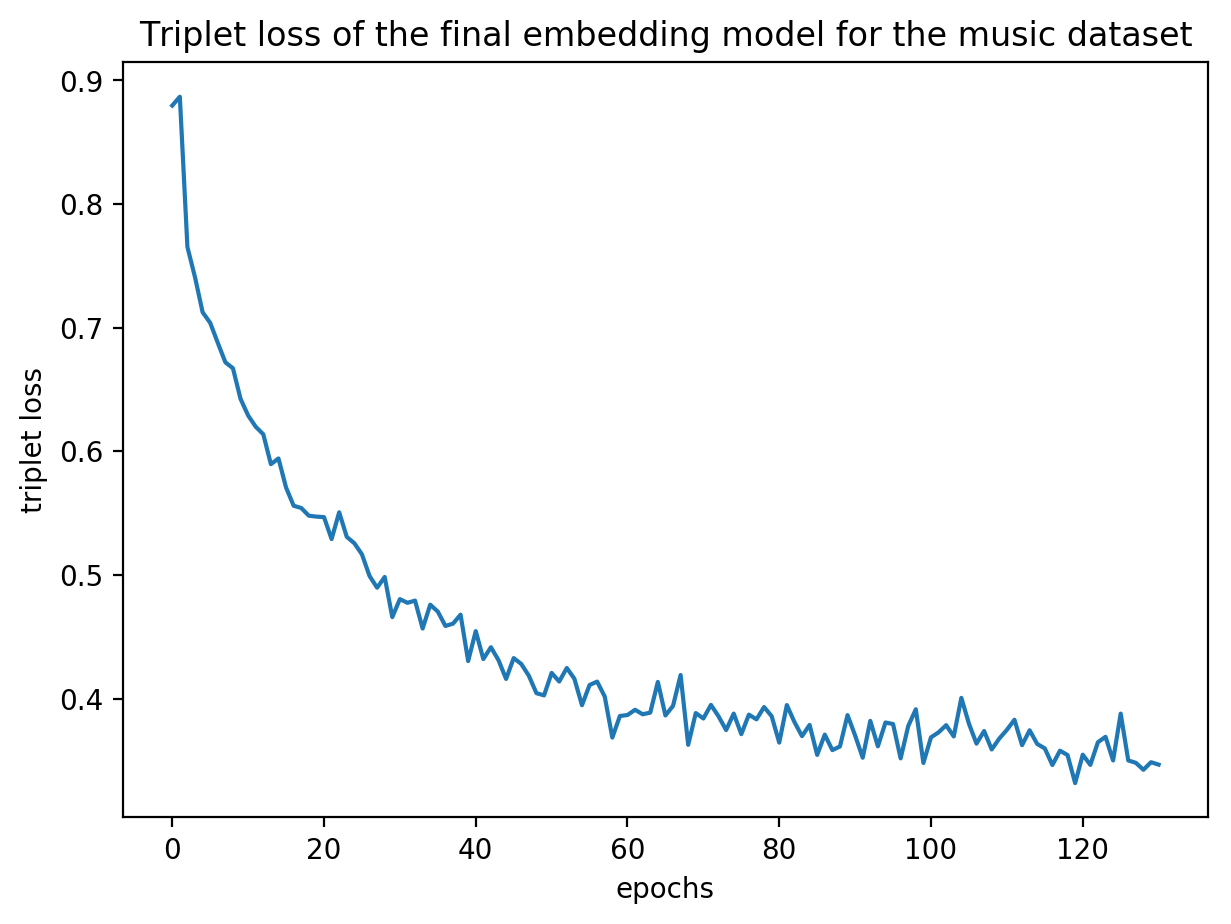
\includegraphics[width=0.6\linewidth]{img/triplet_loss_music_final.png}
    \caption{Triplet loss plot of the final embedding model for the music dataset}
    \label{fig:Triplet-Loss-Music}
\end{figure}

\subsection{Embedding space}
\label{sub:Results-Music-Embedding-Space}
The music embedding space was similarly examined as the noise detection space (\ref{sub:Eval-Embedding-Space-DCASE}). For the examination, the entire dataset was projected onto the embedding space and the value, including the metadata of each point, was saved. The examination was done in a jupyter notebook located in the \texttt{notebooks} folder called \texttt{examination\_embedding\_space.ipynb}.
\newline
\newline
The first part of the examination was to explore the neighbourhood of the embedding space, which was done by building a neighbouring tree using the \texttt{cKDTree} from \texttt{scipy}. Then to examine the neighbourhood, from each of the embedded points its nearest 30 neighbours were checked, and their labels were compared, which aims to find inconsistencies. If a sample had 28 or more different labels in its neighbourhood, it was further examined, since this represents either a malfunction of the embedding space or a significant sample in the dataset, which can be classified as a different genre. These points were then appended with its five nearest neighbours and a song was created, which represents the neighbourhood. This song showed that even if the neighbourhood was inconsistent, the resulting sound did still sound very similar to an amateur. However, since this needs to be evaluated by an expert, these generated songs were used in the qualitative analysis (\ref{sub:Results-Music-Qualitative-analysis}) and evaluated by a professional DJ.
\newline
\newline
The next examination of the embedding space was to compute the centroids of each category cluster, and then taking the five nearest neighbours from each, which will then be used to create a song from all of the segments. This created song should represent a typical song of the specific cluster. For an amateur this it sounds like this is the case, however, this needs to be shown in the qualitative analysis (\ref{sub:Results-Music-Qualitative-analysis}).
\newline
\newline
The last examination of the embedding space was walking through the embedding space, which was already done and described in the section above from the noise detection dataset (\ref{sub:Eval-Embedding-Space-DCASE}). The idea is to walk from cluster to cluster with a specified amount of steps and taking the three next neighbours from each one of the steps. All of the audios were then appended and a this results in a song, which should represent a song with the starting point in a specific cluster and then ends in a different one, where the transitions should sound reasonable. This \flqq walk through the embedding space\frqq \ can further be represented as an image, where the log Mel representation is computed of each of the segments and then appended as a sub-figure to the overall figure. Such an image is shown in figure \ref{fig:Walk-through-Music}. The figure shows, that when purely looking at it, the transitions seem reasonable and a clear build up was noticed to the label \textit{Trance}. However, this needs to be shown in the qualitative analysis (\ref{sub:Results-Music-Qualitative-analysis}) as well. Each combination of categories was computed and the resulting song with the corresponding image of the \flqq walk through the embedding space\frqq \ was saved.
\begin{figure}[ht]
\centering
    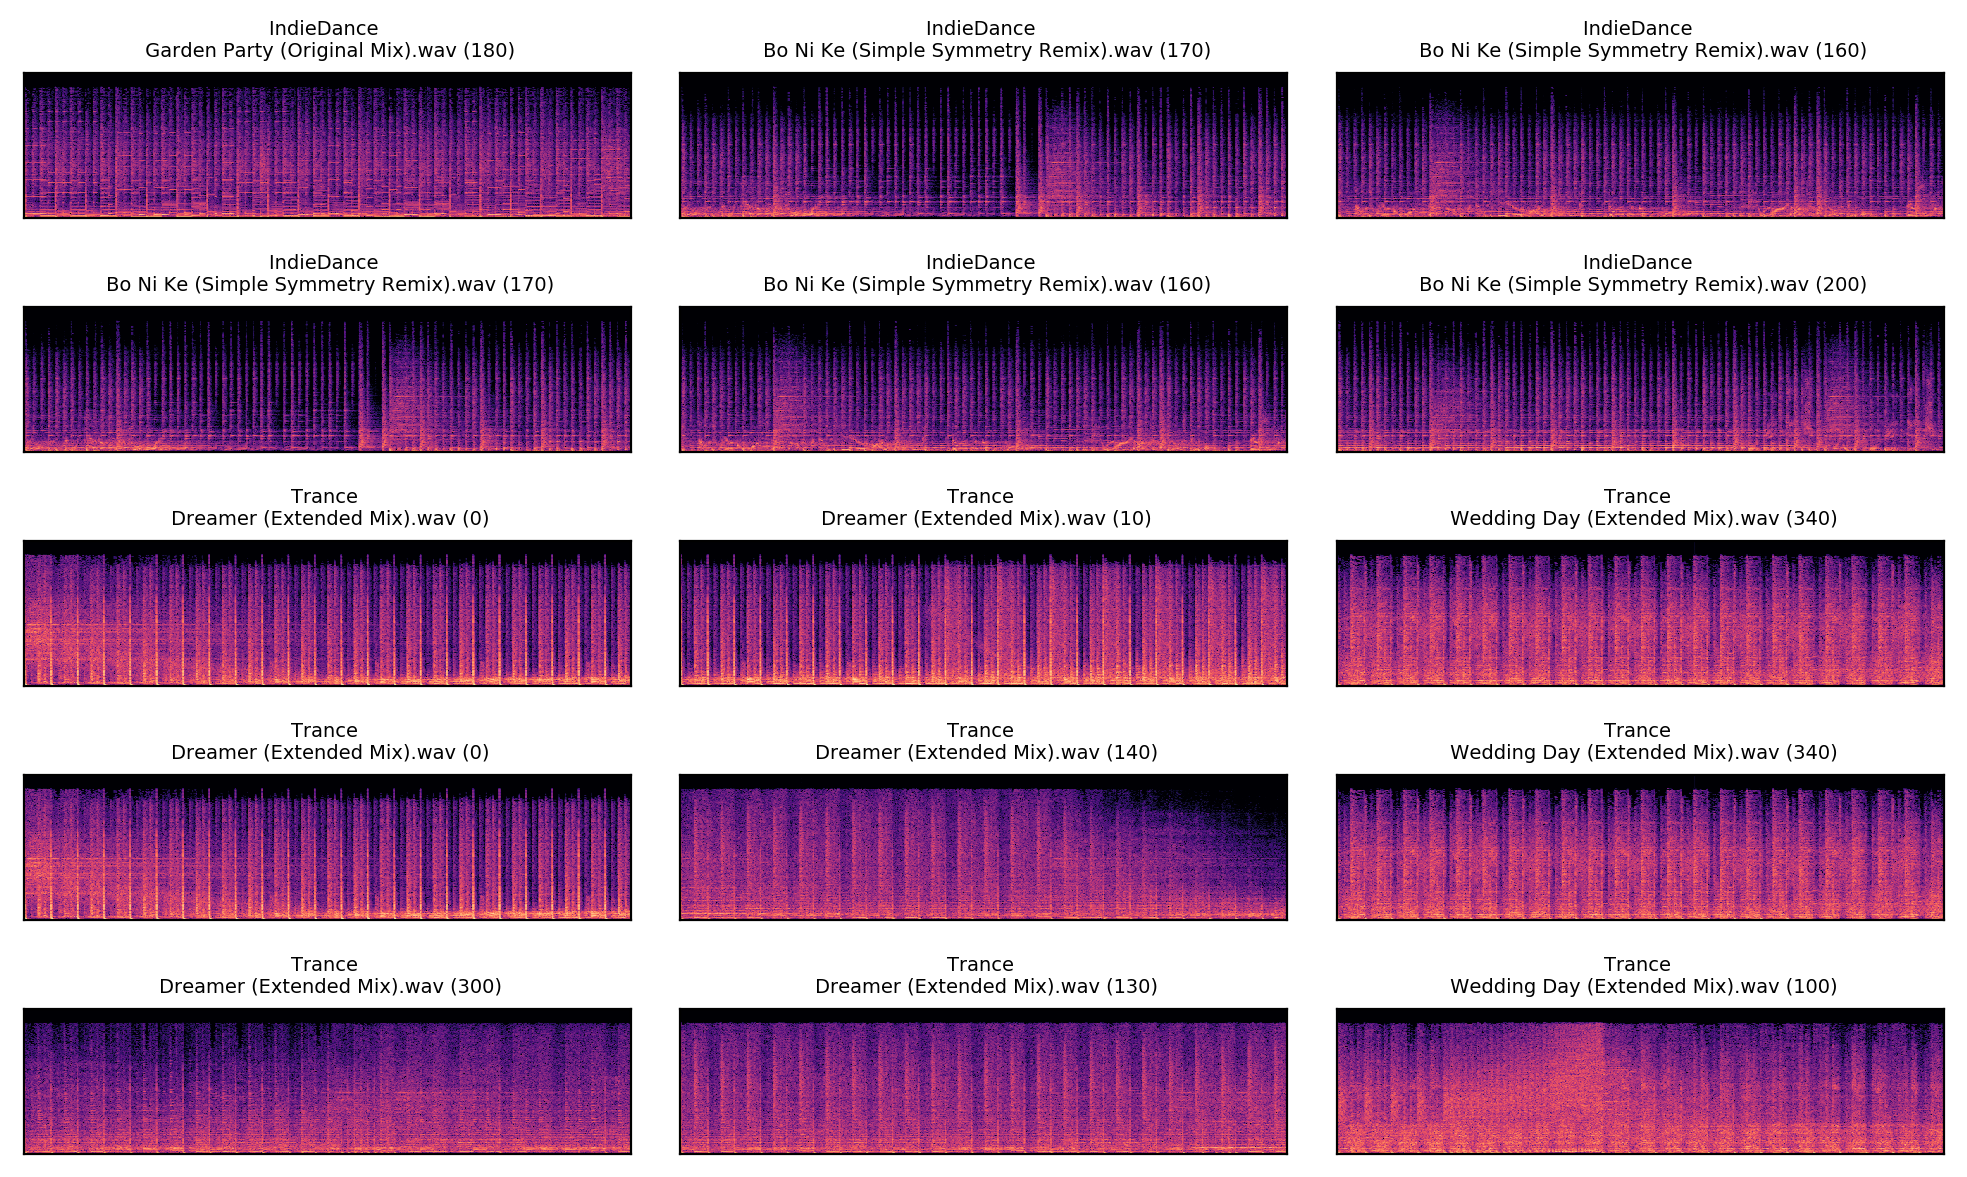
\includegraphics[width=0.9\linewidth]{img/Walk_through_music_space.png}
    \caption{\flqq walk through the embedding space\frqq \ of the music space from \textit{IndieDance} to \textit{Trance}}
    \label{fig:Walk-through-Music}
\end{figure}

\subsection{Clustering applied to embedding space}
\label{sub:Results-Music-Clustering}
\begin{figure}[ht]
\centering
    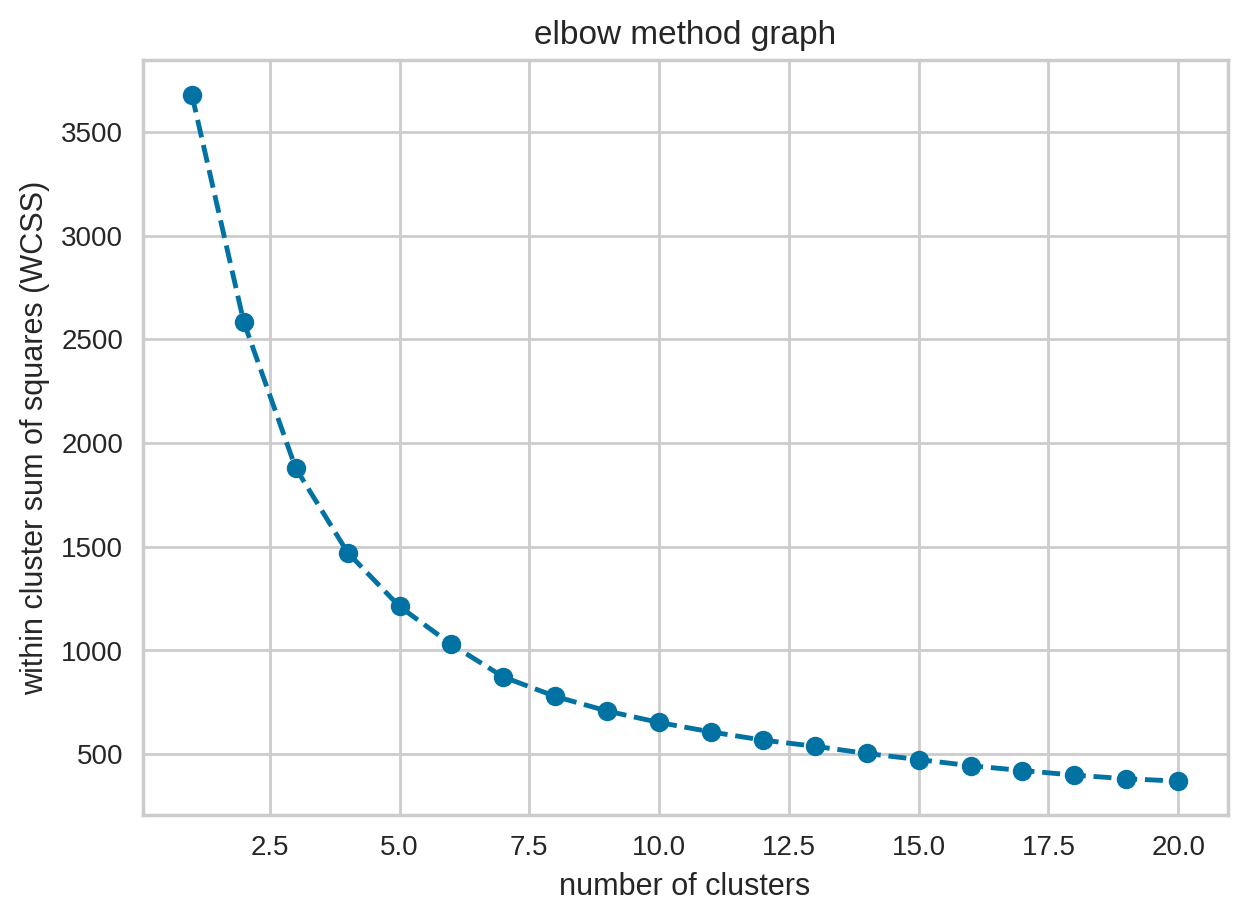
\includegraphics[width=0.6\linewidth]{img/elbow_method_music_dataset.png}
    \caption{Plot of the elbow method on the music embedding space to find the optimal number of clusters}
    \label{fig:Elbow-Clusters}
\end{figure}
\noindent
One of the requirements of the thesis was to apply a standard clustering algorithm to the embedding space and examining the resulting clusters. For this thesis, K-Means is chosen as the clustering algorithm (\ref{sub:K-Means}), since clustering was explicitly excluded from the thesis and only a simple and easy to implement algorithm should be used. To apply clustering to the embedding space and to visualise the results, the dimensionality had to be reduced to at least three dimensions. The dimensionality reduction was done by computing \gls{PCA} and using only three principal components. Afterwards, these three principal components were used to compute the \gls{WCSS}, for the different number of clusters, with results in computing the elbow method, which is used to find the optimal number of clusters. The \gls{WCSS} measures the average squared distance of all the points within a cluster to the cluster centroid. Figure \ref{fig:Elbow-Clusters} shows the plot of the \gls{WCSS} when increasing the number of clusters. The figure shows that the optimal number of classes is between six and seven because this represents the \flqq elbow\frqq \ of the graph. For this evaluation, the optimal number of clusters is chosen to be seven, since this was also the number of different sub-genres in the dataset. Thereafter, K-Means was computed using seven clusters by using the implementation of \texttt{sklearn}. When visualising the cluster, this results in the figure \ref{fig:K-Means-Visualisation}, where the colours represent the clusters and the \flqq x\frqq \ represents the centre of each cluster.
\newline
\newline
The resulting clusters were examined by looking at the distribution of the different labels contained in each. This aims to show which cluster contains which labels. Table \ref{tab:Distribution-KMeans-Clusters} shows the distribution of each of the seven clusters. The clustering result shows that in every cluster, there is a different sub-genre which occurs most frequently. This shows that even with such a simple clustering algorithm, there are separated clusters of each of the seven sub-genres. However, the clusters still contain a fair amount of different labels, which is typical in such entangled categories as the ones in the music dataset.
\begin{figure}[ht]
\centering
    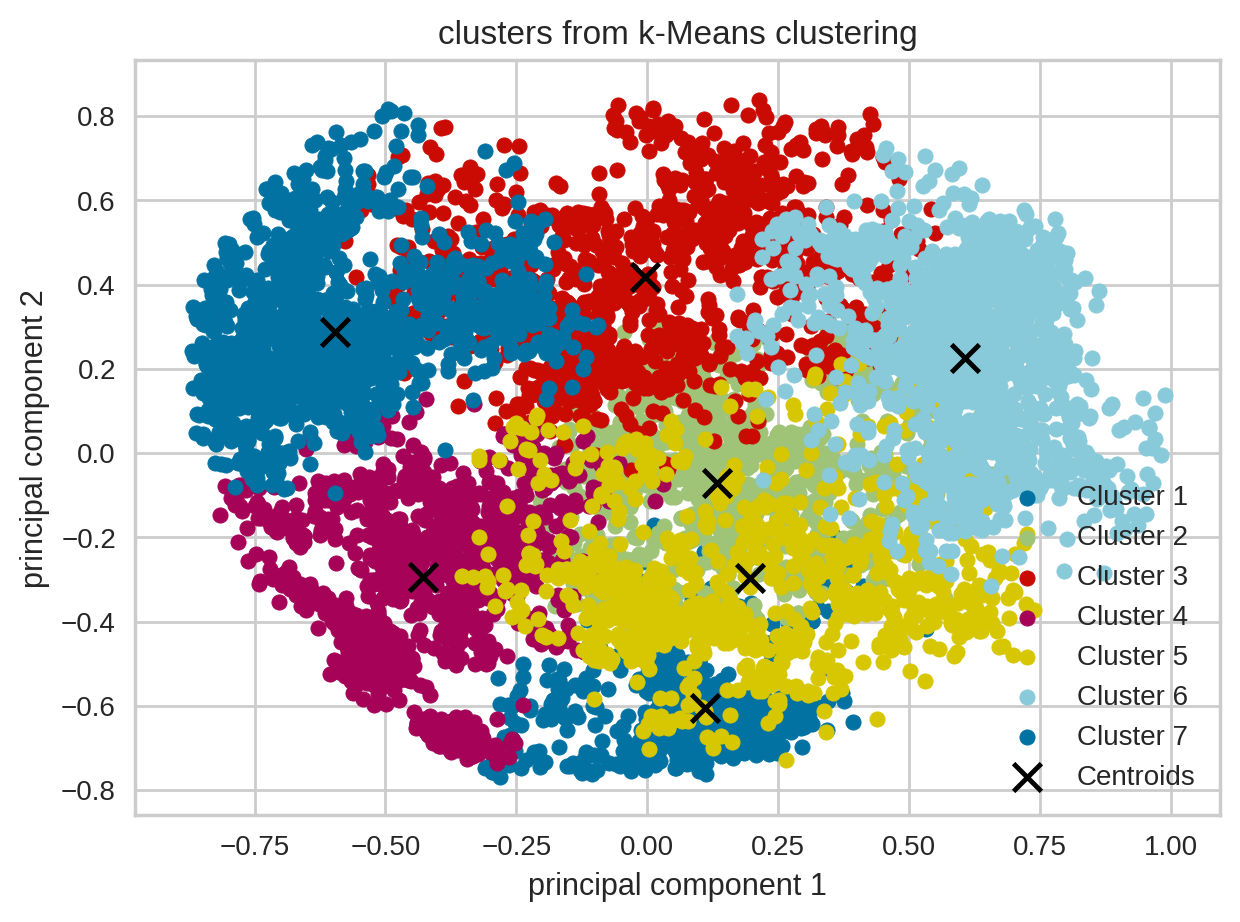
\includegraphics[width=0.8\linewidth]{img/kmeans_music.png}
    \caption{K-Means visualisation of the embedding space}
    \label{fig:K-Means-Visualisation}
\end{figure}
\begin{table}[ht]
    \centering
    \caption{Distribution of the sub-genres in each one of the seven clusters computed with K-Means}
	\label{tab:Distribution-KMeans-Clusters}
    \begin{tabular}{l|l}
        \toprule
        \textbf{cluster id} & \textbf{sub-categories (count of each)} \\ 
        \midrule[1pt]
        1 & \begin{minipage}{4in}
        \vskip 4pt
        MelodicHouseAndTechno (28) \\
        Techno\_Raw\_Deep\_Hypnotic (54) \\
        Trance (711)
        \vskip 4pt
        \end{minipage} \\ 
        \hline
        2 & \begin{minipage}{4in}
        \vskip 4pt
        DeepHouse (183) \\
        Electronica\_Downtempo (139) \\
        IndieDance (451) \\
        MelodicHouseAndTechno (362) \\
        Trance (31)
        \vskip 4pt
        \end{minipage} \\
        \hline
        3 & \begin{minipage}{4in}
        \vskip 4pt
        DeepHouse (395) \\
        Electronica\_Downtempo (112) \\
        IndieDance (99) \\
        MelodicHouseAndTechno (209) \\
        Techno\_PeakTime\_Driving\_Hard (105) \\
        Techno\_Raw\_Deep\_Hypnotic (86) \\
        Trance (115)
        \vskip 4pt
        \end{minipage} \\
        \hline
        4 & \begin{minipage}{4in}
        \vskip 4pt
        DeepHouse (93) \\
        Electronica\_Downtempo (164) \\
        IndieDance (165) \\
        Techno\_PeakTime\_Driving\_Hard (49) \\
        Techno\_Raw\_Deep\_Hypnotic (521) \\
        Trance (62)
        \vskip 4pt
        \end{minipage} \\
        \hline
        5 & \begin{minipage}{4in}
        \vskip 4pt
        DeepHouse (101) \\
        Electronica\_Downtempo (625) \\
        IndieDance (43) \\
        MelodicHouseAndTechno (91) \\
        Techno\_Raw\_Deep\_Hypnotic (53) 
        \vskip 4pt
        \end{minipage} \\
        \hline
        6 & \begin{minipage}{4in}
        \vskip 4pt
        DeepHouse (373) \\
        Electronica\_Downtempo (36) \\
        IndieDance (300) \\
        MelodicHouseAndTechno (644) 
        \vskip 4pt
        \end{minipage} \\
        \hline
        7 & \begin{minipage}{4in}
        \vskip 4pt
        IndieDance (34) \\
        MelodicHouseAndTechno (55) \\
        Techno\_PeakTime\_Driving\_Hard (975) \\
        Techno\_Raw\_Deep\_Hypnotic (174) \\
        Trance (91)
        \vskip 4pt
        \end{minipage} \\
        \bottomrule
    \end{tabular}
\end{table}

\subsection{Qualitative analysis}
\label{sub:Results-Music-Qualitative-analysis}
The qualitative analysis aims to evaluate the embedding space created for music, with the help of en expert. In this thesis the expert is mister Emanuel Oehri, which is a DJ and also kindly provided the music dataset and therefore is very familiar with the sub-genres of the dataset, since he himself picked these out. The qualitative analysis was done in the form of an interview, where the interview guide can be found in the appendix \ref{sec:Interview-Guide}. The key elements of the analysis were summarised and described in this subsection. The detailed interview can be found in the appendix REF.

\subsection{Conclusion}
\label{sub:Results-Music-Conclusion}



\chapter{Conclusion}
\label{ch:Conclusion}

\section{Project conclusion}
\label{sec:Project-Conclusion}

\section{Outlook}
\label{sec:Outlook}



\newpage

\pagenumbering{Roman}

\appendix
% Verhindert das Einfügen von Kapiteltitel kleiner als \chapter
\addtocontents{toc}{\protect\setcounter{tocdepth}{0}}

\listoffigures

\listoftables

\listofmyequations 
\pagebreak

\printglossary[type=\acronymtype, title=List of Abbreviations]

\printbibliography[heading=bibintoc,title=Bibliography]

\chapter{SINS database table}
\label{app:SINS-Database-Table}
This chapter shows a table with the different activities recorded within the SINS database. The activities are divided into the room where they were recorded.

\begin{table}[htbp]
    \centering
    \caption[SINS database recorded activities for each room]{SINS database recorded activities for each room \footnotemark}
	\label{tab:sins-database-recorded-activities}
    \begin{tabular}{l|l|c|c}
        \toprule
        \textbf{Room} & \textbf{Activity} & \textbf{Nr. ex.} & \textbf{duration (min.)} \\ 
        \midrule[1pt]
        \multirow{10}{*}{Living room} & Phone call & 22 & 8.17 $\pm$ 13.73 \\
        \cline{2-4}
        & Cooking & 19 & 16.62 $\pm$ 9.49 \\
        \cline{2-4}
        & Dish washing & 15 & 6.37 $\pm$ 1.49 \\
        \cline{2-4}
        & Eating & 19 & 7.78 $\pm$ 4.27 \\
        \cline{2-4}
        & Visit & 9 & 13.3 $\pm$ 12.11 \\
        \cline{2-4}
        & Watching TV & 13 & 155.38 $\pm$ 93.28 \\
        \cline{2-4}
        & Working & 15 & 31.24 $\pm$ 39.33 \\
        \cline{2-4}
        & Vacuum cleaning & 15 & 4.79 $\pm$ 2.14 \\
        \cline{2-4}
        & Other & 15 & 0.75 $\pm$ 0.95 \\
        \cline{2-4}
        & Absence & 15 & 66.37 $\pm$ 130.30 \\
        \midrule[1pt]
        \multirow{7}{*}{Bathroom} & Drying with towel & 10 & 1.67 $\pm$ 0.28 \\
        \cline{2-4}
        & Shaving & 13 & 1.91 $\pm$ 1.46 \\
        \cline{2-4}
        & Showering & 10 & 6.11 $\pm$ 2.38 \\
        \cline{2-4}
        & Tooth brushing & 19 & 1.41 $\pm$ 0.25 \\
        \cline{2-4}
        & Vacuum cleaning & 9 & 0.87 $\pm$ 0.59 \\
        \cline{2-4}
        & Other & 75 & 0.42 $\pm$ 0.4 \\
        \cline{2-4}
        & Absence & 35 & 248.56 $\pm$ 263.62 \\
        \midrule[1pt]
        \multirow{3}{*}{Hall} & Vacuum cleaning & 9 & 3.31 $\pm$ 1.11 \\
        \cline{2-4}
        & Other & 164 & 0.36 $\pm$ 0.22 \\
        \cline{2-4}
        & Absence & 175 & 50.17 $\pm$ 102.52 \\
        \midrule[1pt]
        \multirow{3}{*}{Toilet} & Toilet visit & 21 & 4.74 $\pm$ 3.24 \\
        \cline{2-4}
        & Vacuum cleaning & 7 & 0.53 $\pm$ 0.07 \\
        \cline{2-4}
        & Absence & 31 & 282.75 $\pm$ 263.19 \\
        \midrule[1pt]
        \multirow{5}{*}{Bedroom} & Dressing & 28 & 1.53 $\pm$ 1.10 \\
        \cline{2-4}
        & Sleeping & 7 & 348.43 $\pm$ 130.73 \\
        \cline{2-4}
        & Vacuum cleaning & 7 & 1.04 $\pm$ 0.27 \\
        \cline{2-4}
        & Other & 22 & 0.27 $\pm$ 0.23 \\
        \cline{2-4}
        & Absence & 22 & 122.28 $\pm$ 157.43 \\
        \bottomrule
    \end{tabular}
\end{table}
\footnotetext{\fullcite{dekkers_sins_2017}}

\chapter{Milestone reports}
\label{app:Milestone-Reports}
This chapter lists the individual milestone reports. These should provide information on the status of the project during the realisation. For every completed milestone, a report was written before the next phase could be started. The table \fullref{tab:Milestones} shows the milestones within the thesis as well as the corresponding dates when the milestone and the phase will be completed and reviewed. The milestones are also shown in the whole project plan in \fullref{fig:Project-Plan}.

\section{Milestone report M1 from the 15.03.2020}
In the first phase of the project, the main goal was to research the subjects used for the thesis. Within phase, the project also had to be initialised and started. More precisely, the project structure and documentation also had to be defined. The goal was also to finish the first chapter of the thesis \fullref{ch:Related-Work} along with the research.

\begin{table}[htbp]
    \centering
    \caption{Work carried out milestone M1 (15.03.2020)}
	\label{tab:Work-Carried-Out-M1}
    \begin{tabular}{p{.70\textwidth} | p{.20\textwidth}}
        \toprule
        \textbf{Task} & \textbf{Status} \\ 
        \midrule[1pt]
        Research: Dataset & finished \\
        \hline
        Research: Audio processing & finished \\
        \hline
        Research: Triplet Loss & finished \\
        \hline
        Research: Tile2Vec & finished \\
        \hline
        Research: Evaluate research & finished \\
        \hline
        Realisation: Project setup & started \\
        \hline
        Realisation: Input pipeline & started \\
        \bottomrule
    \end{tabular}
\end{table}

\subsection{What work was carried out in the last reporting period}
The tasks carried out within this period are shown in the table \fullref{tab:Work-Carried-Out-M1}, along with the status of the task at the time of the milestone review. A detailed report on the entire tasks carried out within the period is shown in the work journal \ref{tab:Work-Journal}. To reach the goal of simultaneously finishing the chapter \ref{ch:Related-Work} with the research, each researched topic was documented right away. 
\subsection{State of progress}
The current milestone was successfully reached since all the planned tasks could be finished. The phase was finished too early so that the next period could already be started, the realisation phase. 

\subsection{Top three risks including planned measures}
\begin{enumerate}
    \setlength\itemsep{0em}
    \item Formulas related work wrong, will be checked by Daniel Pfäffli
    \item Topics missing in related work, will be checked by Daniel Pfäffli
    \item Input pipeline structure, will be discussed at the next meeting
\end{enumerate}

\section{Milestone report M2 from the 29.03.2020}
In the second milestone of the project, the main goal was to finish the whole project setup. The project repository had to be set up, the input pipeline was created for the dataset, and the default model architecture was created. The purpose was that after this milestone, the project is at a certain point, that the implementation of specific architectures is fast enough to experiment with different ones.

\begin{table}[htbp]
    \centering
    \caption{Work carried out milestone M2 (29.03.2020)}
	\label{tab:Work-Carried-Out-M2}
    \begin{tabular}{p{.70\textwidth} | p{.20\textwidth}}
        \toprule
        \textbf{Task} & \textbf{Status} \\ 
        \midrule[1pt]
        Realisation: Project setup & finished \\
        \hline
        Realisation: Input pipeline & finished \\
        \hline
        Realisation: Default architecture & finished \\
        \hline
        Realisation: Evaluation Workflow & midway \\
        \hline
        Realisation: Unit tests & midway \\
        \bottomrule
    \end{tabular}
\end{table}

\subsection{What work was carried out in the last reporting period}
The tasks carried out within this period are shown in the table \fullref{tab:Work-Carried-Out-M2}, along with the status of the task at the time of the milestone review. A detailed report on the entire tasks carried out within the period is shown in the work journal \ref{tab:Work-Journal}. Two tasks were not completed within the period, which was now prioritised in the next phase and will get completed first. The milestone could not be completed because to little time was planned for tasks like \flqq input pipeline\frqq or \flqq evaluation workflow\frqq. The evaluation workflow was completed except for the classifier, to evaluate the architecture in relation to the other models in the DCASE Challenge. Unit tests were not written for all the created models but will be right away at the start of the next milestone.

\subsection{State of progress}
The current milestone was not reached since two tasks could not be finished entirely. The uncompleted tasks were prioritised and were moved to the next phase of the project.

\subsection{Top three risks including planned measures}
\begin{enumerate}
    \setlength\itemsep{0em}
    \item GPU caching / file deletion problem, will be discussed at the next meeting
    \item Classifier architecture, will be discussed at the next meeting
    \item Unit tests for models, will be discussed at the next meeting 
\end{enumerate}

\section{Milestone report M3 from the 12.04.2020}
The third milestone aimed to finalise the realisation. The idea of unsupervised triplet loss had to be implemented, like the one from Tile2Vec for both datasets. Furthermore, an easy to use architecture for the experiments had to be developed. Thus the experiments should be conducted relatively simple. The main goal is to provide an architecture which is reliable, arbitrarily expandable and repeatable. All of these points are essential for conducting successful experiments.

\begin{table}[htbp]
    \centering
    \caption{Work carried out milestone M3 (12.04.2020)}
	\label{tab:Work-Carried-Out-M3}
    \begin{tabular}{p{.70\textwidth} | p{.20\textwidth}}
        \toprule
        \textbf{Task} & \textbf{Status} \\ 
        \midrule[1pt]
        Realisation: Evaluation Workflow & finished \\
        \hline
        Realisation: Unit tests & finished \\
        \hline
        Realisation: Tile2Vec implementation & finished \\
        \hline
        Realisation: Architecture for experiments & finished \\
        \hline
        Experiments: Conduct experiments & started \\
        \bottomrule
    \end{tabular}
\end{table}

\subsection{What work was carried out in the last reporting period}
The tasks carried out within this period are shown in the table \fullref{tab:Work-Carried-Out-M3}, along with the status of the task at the time of the milestone review. A detailed report on the entire tasks carried out within the period is shown in the work journal \ref{tab:Work-Journal}. Two tasks were not completed during the last phase and were completed at the start of this phase by prioritising them. Both of the other tasks which were planned to complete during this phase were completed.

\subsection{State of progress}
The current milestone was successfully reached since all the planned tasks could be finished. The phase was finished too early so that the next period could already be started, the experiment phase. 

\subsection{Top three risks including planned measures}
\begin{enumerate}
    \setlength\itemsep{0em}
    \item Review evaluation workflow, will be discussed at the next meeting
    \item Review of study doc, will be discussed at the next meeting
    \item Review of test concept, will be discussed at the next meeting 
\end{enumerate}

\section{Milestone report M5 from the 03.05.2020}
The last milestone before the thesis submission is the M5, which concludes the experiment phase. In the experiment phase, all of the experiments are conducted and validated. For each experiment, a separate study doc is written, which describes the experiments in more detail, and can be found in \ref{app:Study-Doc}. Within this phase, a lot of different experiments are conducted to find the optimal parameters for the problem definition. In this phase, the codebase will be adjusted if problems are found or if new ideas need to be implemented. The purpose of these adjustments is always to improve the performance of the models.
\begin{table}[htbp]
    \centering
    \caption{Work carried out milestone M5 (03.05.2020)}
	\label{tab:Work-Carried-Out-M5}
    \begin{tabular}{p{.70\textwidth} | p{.20\textwidth}}
        \toprule
        \textbf{Task} & \textbf{Status} \\ 
        \midrule[1pt]
        Experiments: Conduct experiments & midway \\
        \hline
        Experiments: Validate experiments & midway \\
        \bottomrule
    \end{tabular}
\end{table}

\subsection{What work was carried out in the last reporting period}
The tasks carried out within this period are shown in the table \fullref{tab:Work-Carried-Out-M5}, along with the status of the task at the time of the milestone review. A detailed report on the entire tasks carried out within the period is shown in the work journal \ref{tab:Work-Journal}. Both of the tasks were not completed during the phase. That the tasks were not completed is because there were more experiments to conduct than intentionally thought. There was also the problem that some of the experiments took a long time to be conducted due to the lack of additional computing resources. Both tasks will be prioritised and completed in the next phase. 

\subsection{State of progress}
The current milestone was not reached since two tasks could not be finished entirely. The uncompleted tasks were prioritised and were moved to the next phase of the project.

\subsection{Top three risks including planned measures}
\begin{enumerate}
    \setlength\itemsep{0em}
    \item Not enough time to conduct all experiments; therefore the buffer phase will be used to conduct additional experiments
    \item Not enough time to conduct all experiments; therefore additional computing power will be rented at \texttt{vast.ai}
    \item Not enough experience with the hyperparameters; therefore will be discussed within the next meeting
\end{enumerate}

\chapter{Test concept}
\label{app:Test-Concept}

\clearpage
\landscapevalues

\begin{table}[htbp]
    \centering
    \caption{Test concept}
	\label{tab:Test-Concept}
    \begin{tabular}{p{.15\textwidth} | p{.40\textwidth} | p{.05\textwidth} | p{.15\textwidth} | p{.15\textwidth}}
        \toprule
        \textbf{Test case} & \textbf{Steps} & \textbf{Status} & \textbf{Expected result} & \textbf{Actual result} \\ 
        \midrule[1pt]
        DCASE iterator & 
        \begin{minipage}{5in}
        \vskip 4pt
        \begin{enumerate}
        \setlength\itemsep{0em}
        \item get dataset from model factory
        \item loop over dataset using for loop
        \item check if the entries are not \texttt{None}
        \end{enumerate}
        \vskip 4pt
        \end{minipage} & \cellcolor{green!30!white}passed & entries available & entries available \\
    \hline
        DCASE triplets & 
        \begin{minipage}{5in}
        \vskip 4pt
        \begin{enumerate}
        \setlength\itemsep{0em}
        \item get dataset from model factory
        \item loop over dataset using for loop
        \item for each entry in the dataset load triplets
        \item loop over resulting triplets
        \item check if there are three triplets
        \item check if all constituents have dimension two 
        \end{enumerate}
        \vskip 4pt
        \end{minipage} & \cellcolor{green!30!white}passed & dataset generates valid triplets & valid triplets generated \\
        \bottomrule
    \end{tabular}
\end{table}

\clearpage
\defaultpagestyle

\chapter{Study doc}
\label{app:Study-Doc}
This chapter contains all of the study docs from the conducted experiments, they include detailed information about each one of the experiments as well as the conclusion out of each.

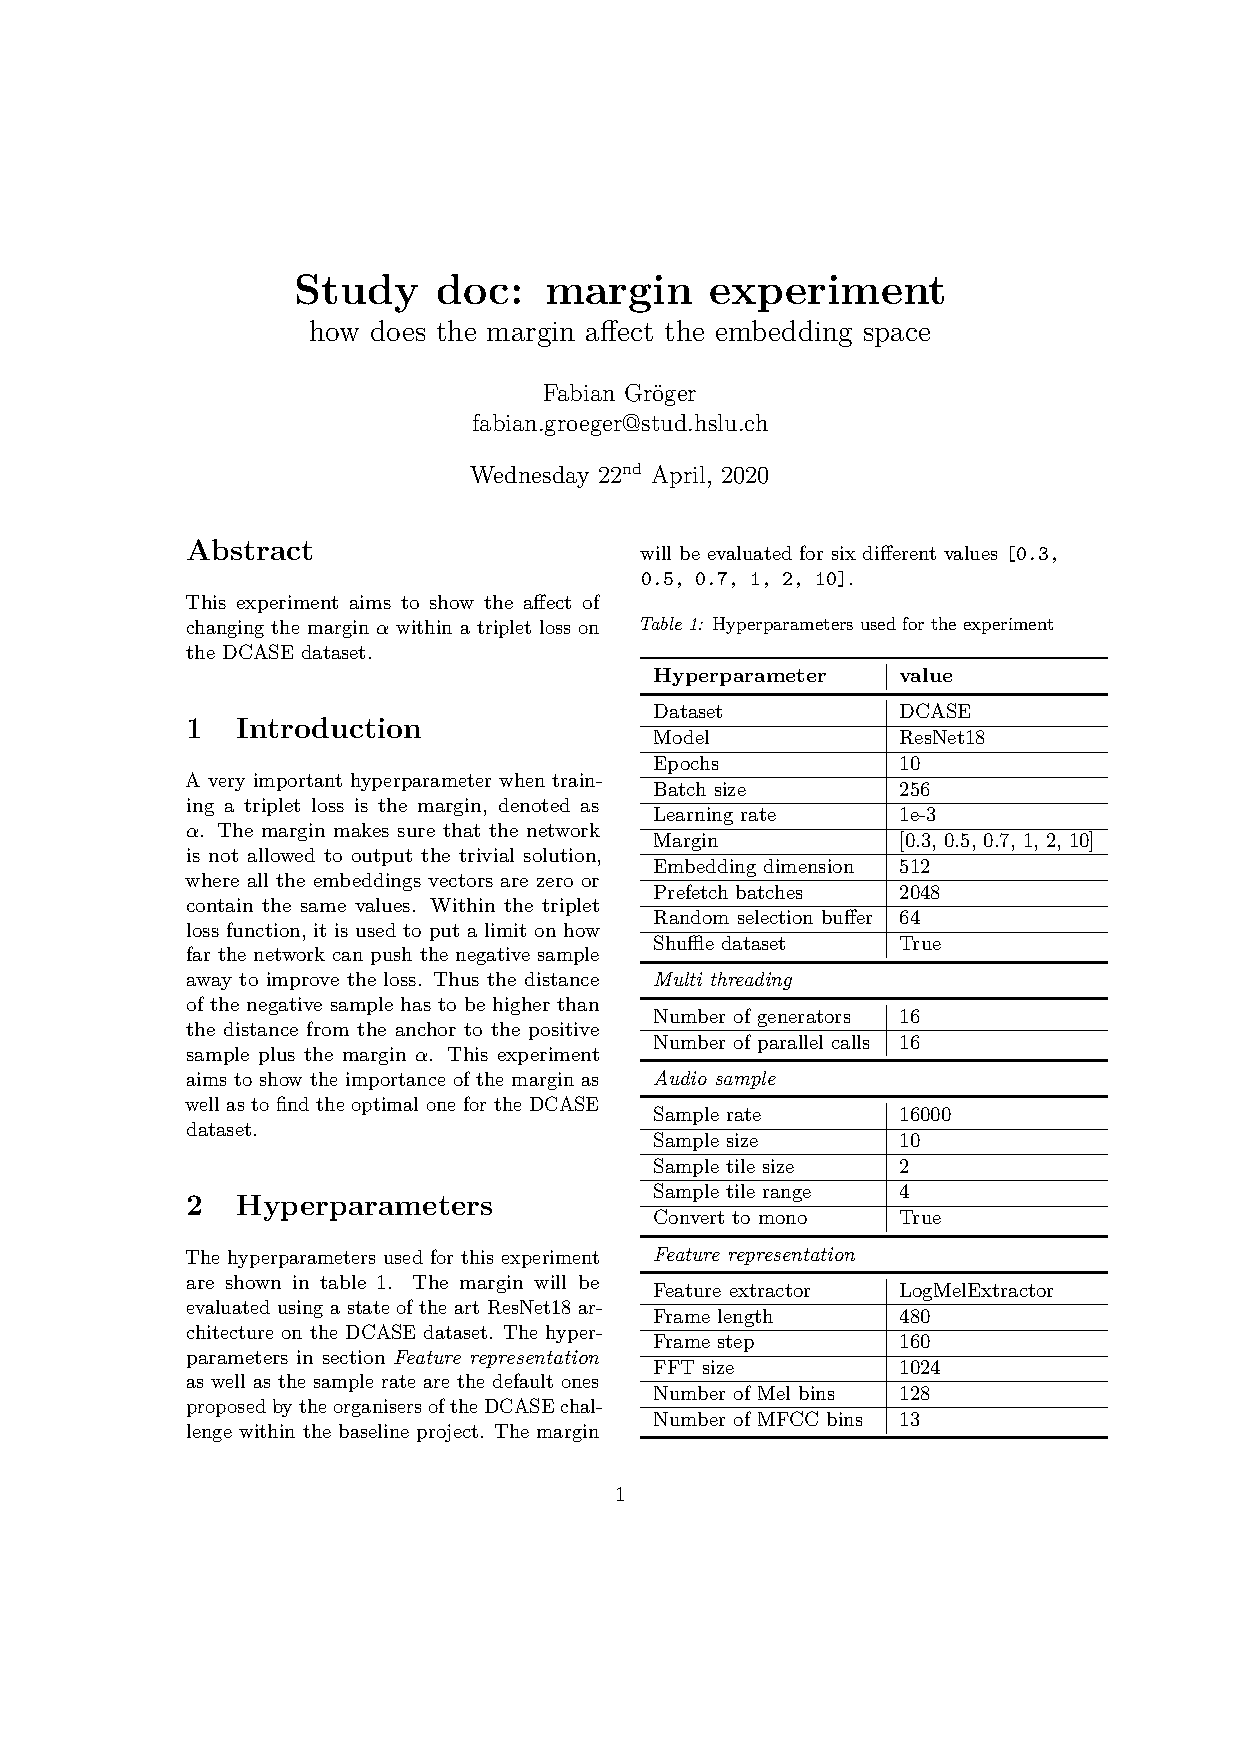
\includepdf[scale=1.0, pages=1-]{study-doc/experiment_margin/Study_Doc_Margin.pdf}

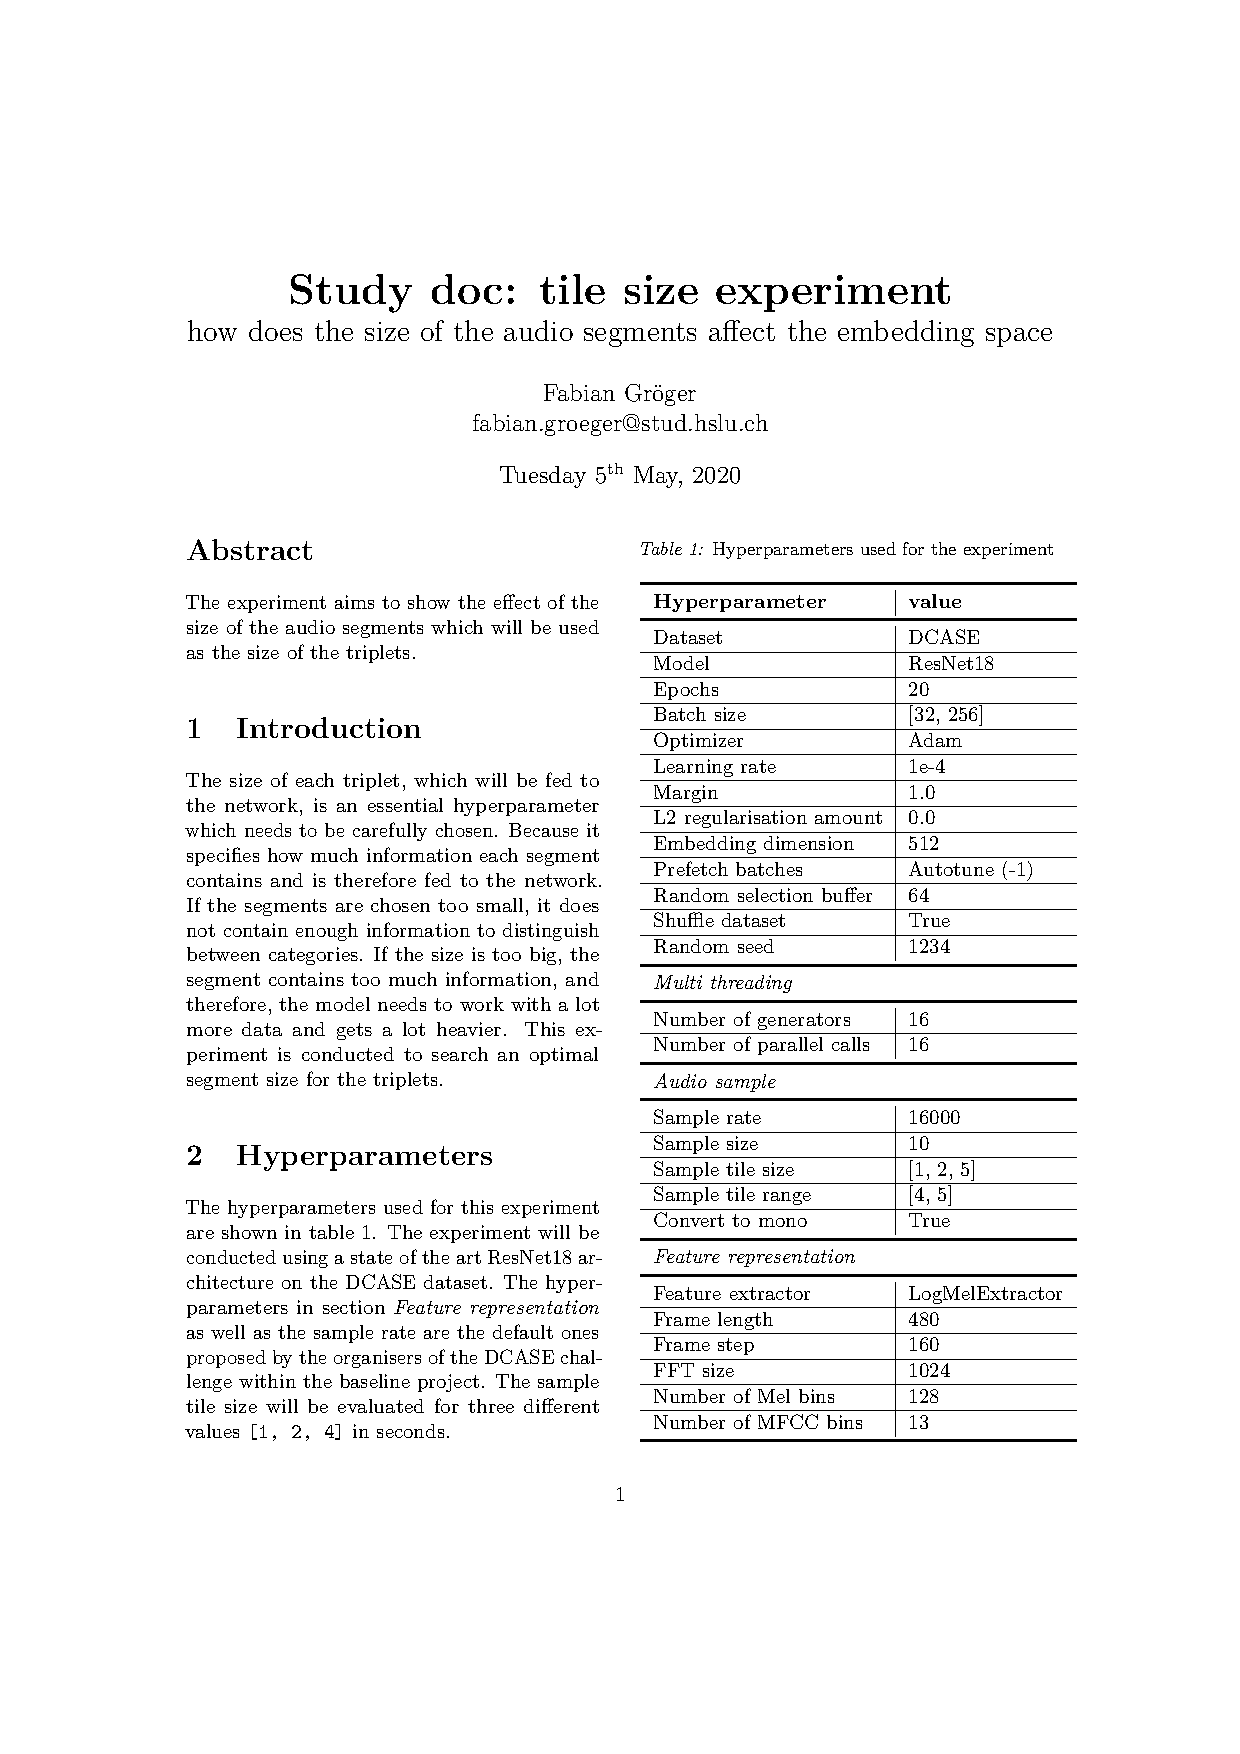
\includepdf[scale=1.0, pages=1-]{study-doc/experiment_tile_size/Study_Doc_tile_size.pdf}

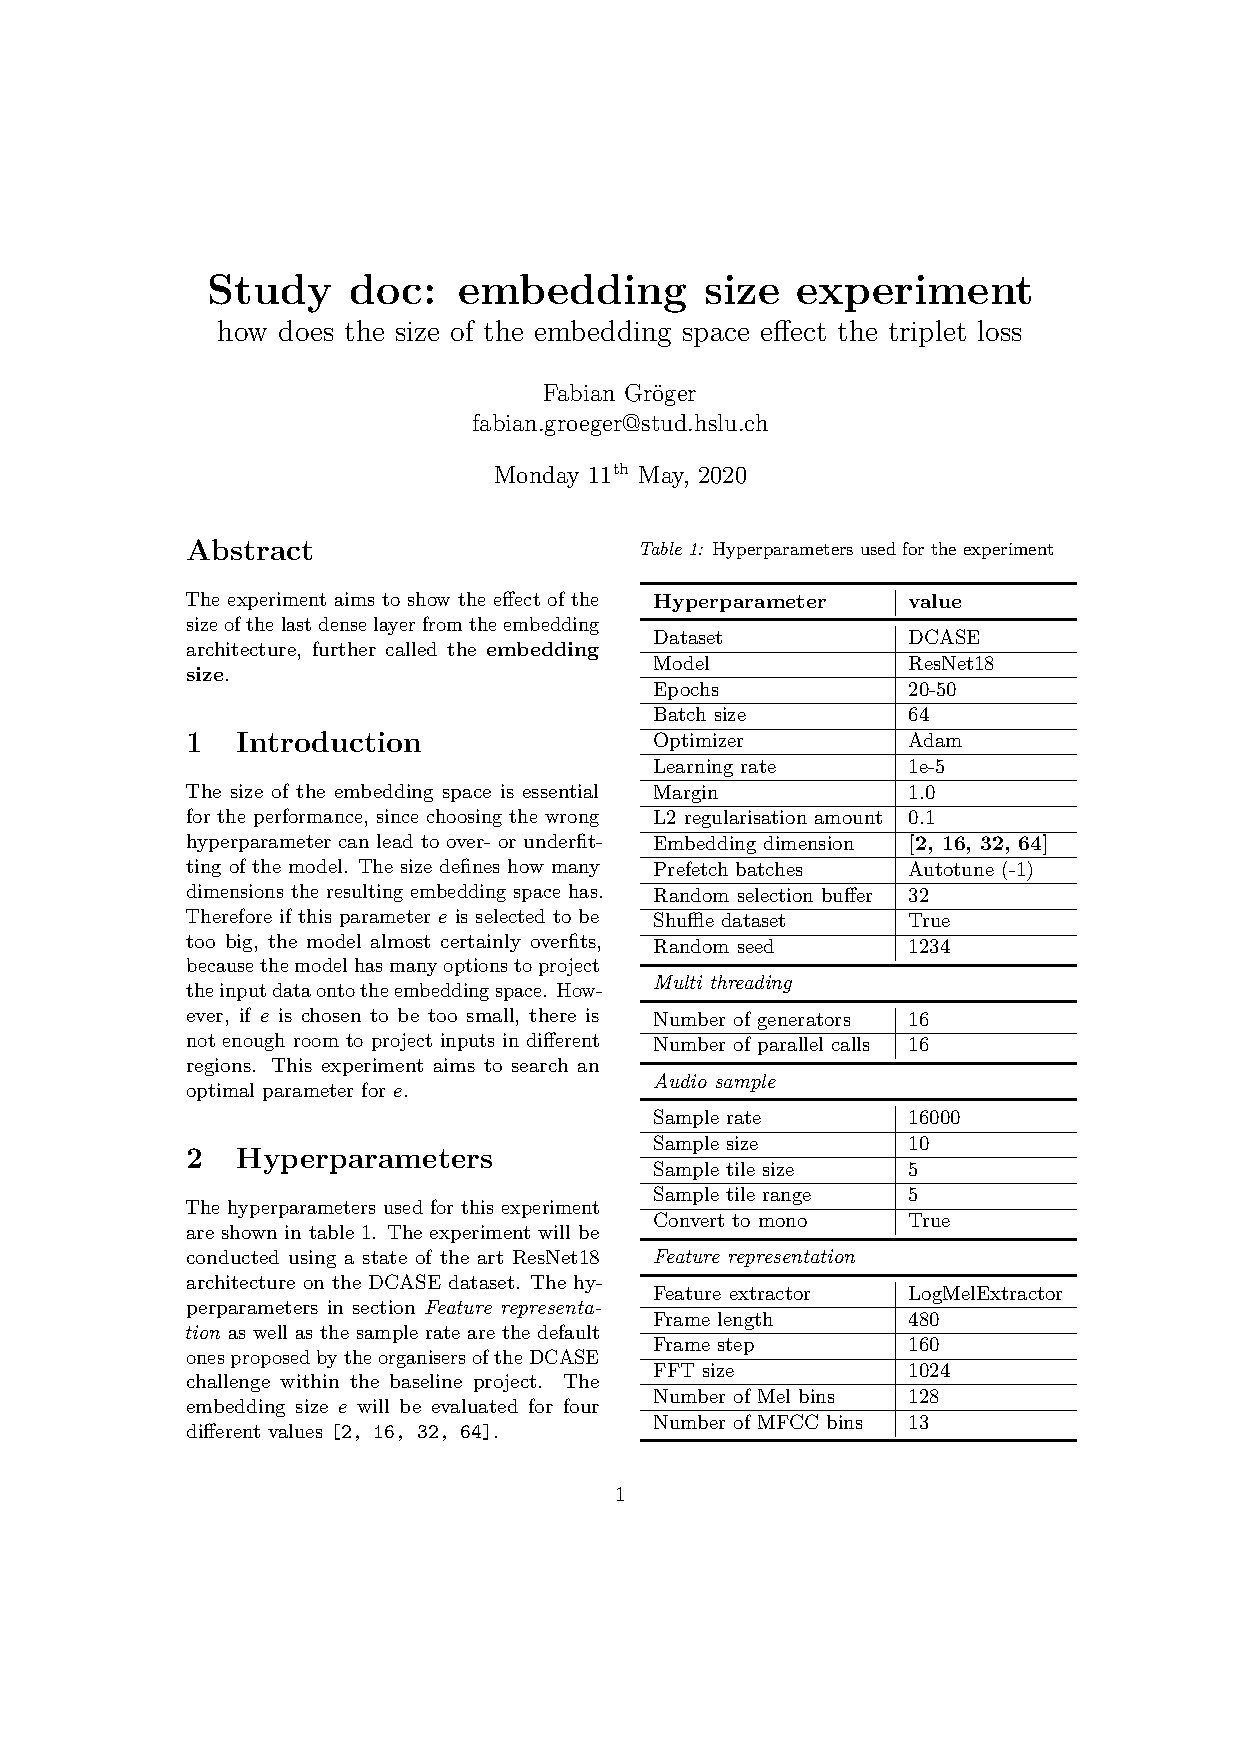
\includepdf[scale=1.0, pages=1-]{study-doc/experiment_embedding_size/Study_Doc_embedding_size.pdf}

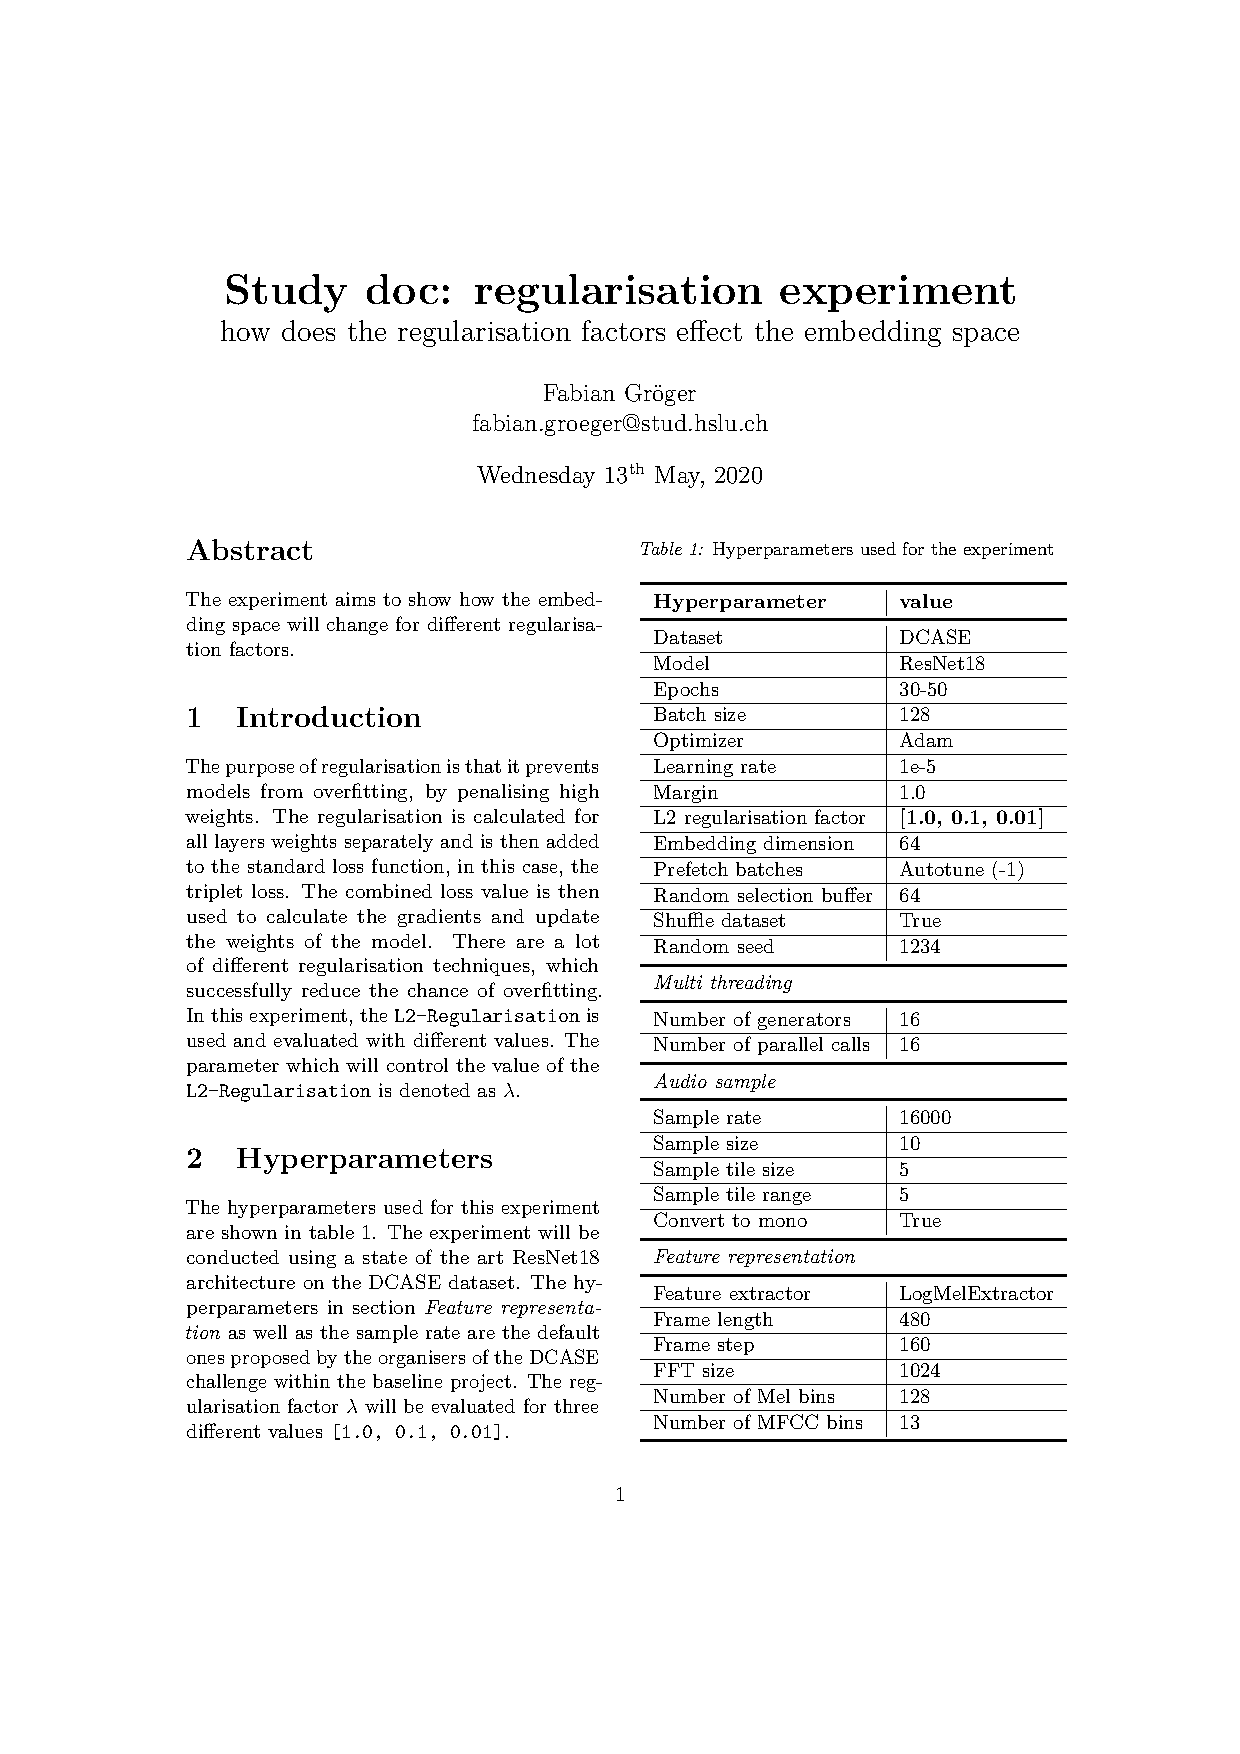
\includepdf[scale=1.0, pages=1-]{study-doc/experiment_regularisation/Study_Doc_regularisation.pdf}

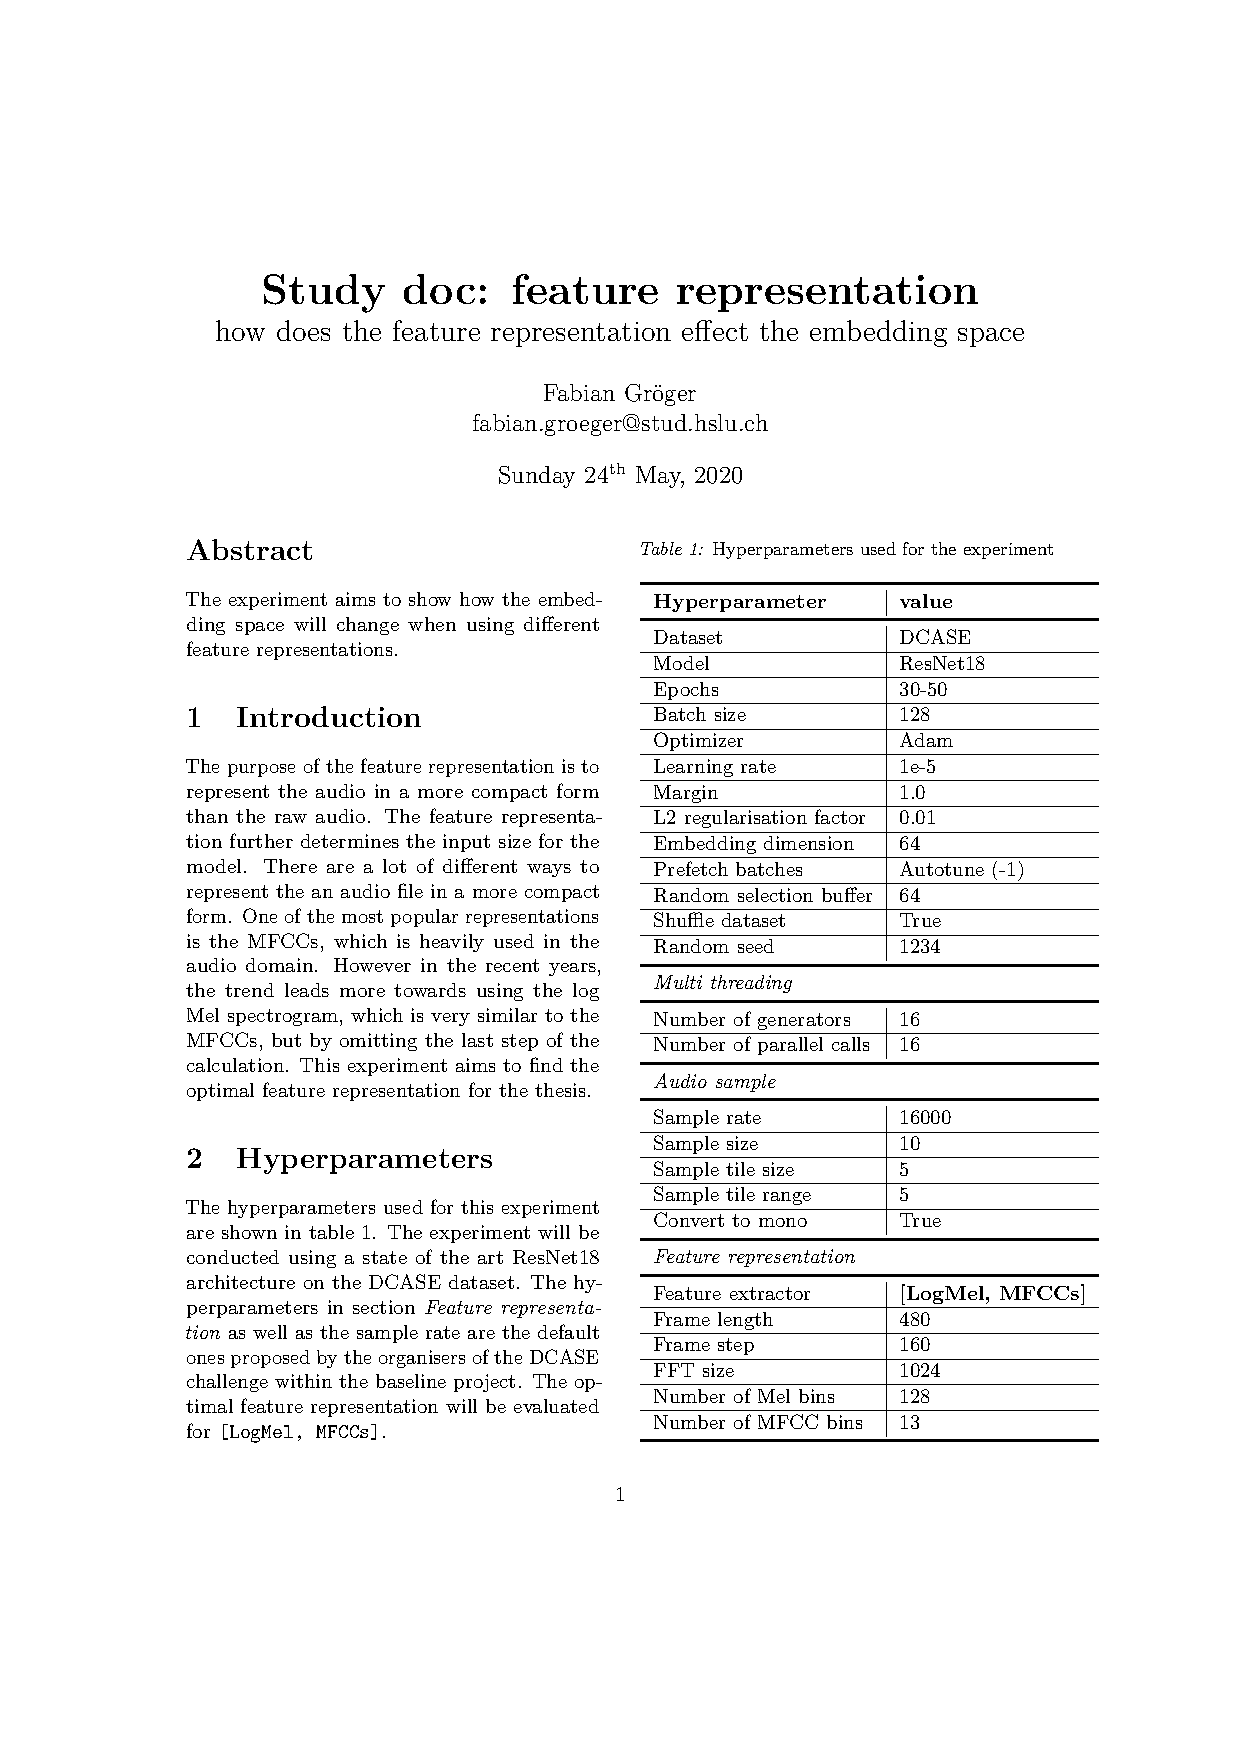
\includepdf[scale=1.0, pages=1-]{study-doc/experiment_feature/Study_Doc_feature_representation.pdf}

\chapter{Qualitative analysis}
\label{app:Qualitative-analysis}

\section{Interview guide}
\label{sec:Interview-Guide}

\includepdf[scale=1.0, pages=1-]{files/bachelor_thesis_interview.pdf}

\chapter{Detailed hyperparameters of the models}
\label{app:detailed-hyperparameters}

\section{DCASE}
\label{app:detailed-hyperparameters-dcase}
\begin{table}[ht]
    \centering
    \caption{Hyperparameters of the optimal embedding architecture for the noise detection dataset}
	\label{tab:Hyperparameters-Detailed-DCASE}
    \begin{tabular}{l|l}
        \toprule
        \textbf{Hyperparameter} & \textbf{value} \\ 
        \midrule[1pt]
        Dataset & DCASE \\
        \hline
        Model & ResNet18 \\ 
        \hline
        Epochs & 110 \\ 
        \hline
        Batch size & 64 \\ 
        \hline
        Optimizer & Adam \\ 
        \hline
        Learning rate & 1e-5 \\
        \hline
        Margin & 1.0 \\
        \hline
        L2 regularisation amount & 0.01 \\
        \hline
        Embedding dimension & 256 \\
        \hline
        Prefetch batches & Autotune (-1) \\ 
        \hline
        Random selection buffer & 32 \\ 
        \hline
        Shuffle dataset & True \\
        \hline
        Random seed & 1234 \\
        \midrule[1pt]
        \multicolumn{2}{l}{\textit{Multi threading}} \\
        \midrule[1pt]
        Number of generators & 16 \\ 
        \hline
        Number of parallel calls & 16 \\
        \midrule[1pt]
        \multicolumn{2}{l}{\textit{Audio sample}} \\
        \midrule[1pt]
        Sample rate & 16000 \\ 
        \hline
        Sample size & 10 \\
        \hline
        Sample tile size & 5 \\
        \hline
        Sample tile range & 5 \\
        \hline
        Convert to mono & True \\
        \midrule[1pt]
        \multicolumn{2}{l}{\textit{Feature representation}} \\
        \midrule[1pt]
        Feature extractor & LogMelExtractor \\ 
        \hline
        Frame length & 480 \\
        \hline
        Frame step & 160 \\
        \hline
        FFT size & 1024 \\
        \hline
        Number of Mel bins & 128 \\
        \hline
        Number of MFCC bins & 13 \\
        \bottomrule
    \end{tabular}
\end{table}

\chapter{Work journal}
\label{app:Work-Journal}

Within this chapter, the whole work journal of the thesis is shown. The journal is divided into subcategories, so that the \fullref{tab:Work-Journal} is more pleased to read. These categories show what exactly was done in the different project phases, which can be seen in the \fullref{fig:Project-Plan}. There is also one more category called \flqq General\frqq, where all the administrative tasks are shown, including the meetings with the advisor.

\clearpage
\landscapevalues

\begin{longtable}{| p{.10\textwidth} | p{.20\textwidth} | p{.50\textwidth} | p{.10\textwidth} |} 
	\caption{Work Journal}
	\label{tab:Work-Journal} \\
    \hline
    \textbf{Date} &
    \textbf{Task} &
    \textbf{Details} &
    \textbf{No. hours} \\
    \hline
    \multicolumn{4}{|l|}{\textbf{General}} \\
    \hline
    17.02.2020 & Preparation for Kick-Off Meeting & 
        \begin{minipage}{5in}
        \vskip 4pt
        \begin{itemize}
        \setlength\itemsep{0em}
        \item thesis description read carefully again
        \item questions of unclear matters
        \end{itemize}
        \vskip 4pt
        \end{minipage}
        & 1h  \\
    \hline
    17.02.2020 & Kick-Off Meeting (number 1)& 
        \begin{minipage}{5in}
        \vskip 4pt
        \begin{itemize}
        \setlength\itemsep{0em}
        \item discussed different topics which are important for the implementation of the project
        \end{itemize}
        \vskip 4pt
        \end{minipage}
        & 1h 30min  \\
    \hline
    24.02.2020 & Meeting (number 2) & 
        \begin{minipage}{5in}
        \vskip 4pt
        \begin{itemize}
        \setlength\itemsep{0em}
        \item preparation of the meeting
        \item meeting itself
        \end{itemize}
        \vskip 4pt
        \end{minipage}
        & 2h  \\
    \hline
    02.03.2020 & Meeting (number 3) & 
        \begin{minipage}{5in}
        \vskip 4pt
        \begin{itemize}
        \setlength\itemsep{0em}
        \item preparation of the meeting
        \item meeting itself
        \end{itemize}
        \vskip 4pt
        \end{minipage}
        & 2h  \\
    \hline
    02.03.2020 & Meeting GPU with Thomas Koller & 
        \begin{minipage}{5in}
        \vskip 4pt
        \begin{itemize}
        \setlength\itemsep{0em}
        \item preparation of the meeting
        \item meeting itself
        \end{itemize}
        \vskip 4pt
        \end{minipage}
        & 0.5h  \\
    \hline
    09.03.2020 & Meeting (number 4) & 
        \begin{minipage}{5in}
        \vskip 4pt
        \begin{itemize}
        \setlength\itemsep{0em}
        \item preparation of the meeting
        \item meeting itself
        \end{itemize}
        \vskip 4pt
        \end{minipage}
        & 2h  \\
    \hline
    16.03.2020 & Meeting (number 5) & 
        \begin{minipage}{5in}
        \vskip 4pt
        \begin{itemize}
        \setlength\itemsep{0em}
        \item preparation of the meeting
        \item meeting itself
        \end{itemize}
        \vskip 4pt
        \end{minipage}
        & 2h  \\
    \hline
    23.03.2020 & Meeting (number 6) & 
        \begin{minipage}{5in}
        \vskip 4pt
        \begin{itemize}
        \setlength\itemsep{0em}
        \item preparation of the meeting
        \item meeting itself
        \end{itemize}
        \vskip 4pt
        \end{minipage}
        & 2h  \\
    \hline
    30.03.2020 & Meeting (number 7) & 
        \begin{minipage}{5in}
        \vskip 4pt
        \begin{itemize}
        \setlength\itemsep{0em}
        \item preparation of the meeting
        \item meeting itself
        \end{itemize}
        \vskip 4pt
        \end{minipage}
        & 2h  \\
    \hline
    06.04.2020 & Meeting (number 8) & 
        \begin{minipage}{5in}
        \vskip 4pt
        \begin{itemize}
        \setlength\itemsep{0em}
        \item preparation of the meeting
        \item meeting itself
        \end{itemize}
        \vskip 4pt
        \end{minipage}
        & 2h  \\
    \hline
    15.04.2020 & Meeting (number 9) & 
        \begin{minipage}{5in}
        \vskip 4pt
        \begin{itemize}
        \setlength\itemsep{0em}
        \item preparation of the meeting
        \item meeting itself
        \end{itemize}
        \vskip 4pt
        \end{minipage}
        & 2h  \\
    \hline
    \multicolumn{4}{|l|}{\textbf{Documentation}} \\
    \hline
    17.02.2020 & Documentation setup & 
        \begin{minipage}{5in}
        \vskip 4pt
        \begin{itemize}
        \setlength\itemsep{0em}
        \item project setup
        \item latex document setup
        \item German transcribed to English
        \item built default documentation structure
        \end{itemize}
        \vskip 4pt
        \end{minipage}
        & 2h  \\
    \hline
    19.02.2020 & Dataset documented & 
        \begin{minipage}{5in}
        \vskip 4pt
        \begin{itemize}
        \setlength\itemsep{0em}
        \item SINS Database
        \item DCASE Task dataset
        \end{itemize}
        \vskip 4pt
        \end{minipage}
        & 3h  \\
    \hline
    24.02.2020 & Dataset section finished & 
        \begin{minipage}{5in}
        \vskip 4pt
        \begin{itemize}
        \setlength\itemsep{0em}
        \item Created table of the recorded activities in the \gls{SINS} database
        \item Reread section and corrected
        \end{itemize}
        \vskip 4pt
        \end{minipage}
        & 1h  \\
    \hline
    02.03.2020 & Triplet Loss section finished & 
        \begin{minipage}{5in}
        \vskip 4pt
        \begin{itemize}
        \setlength\itemsep{0em}
        \item Documented Triplet Loss in related work
        \item Reread section and corrected
        \end{itemize}
        \vskip 4pt
        \end{minipage}
        & 2h  \\
    \hline
    03.03.2020 & Tile2Vec section finished & 
        \begin{minipage}{5in}
        \vskip 4pt
        \begin{itemize}
        \setlength\itemsep{0em}
        \item Documented Tile2Vec in related work
        \item Reread section and corrected
        \item Corrected equations
        \end{itemize}
        \vskip 4pt
        \end{minipage}
        & 2h  \\
    \hline
    05.03.2020 & Started with intro to neural networks & 
        \begin{minipage}{5in}
        \vskip 4pt
        \begin{itemize}
        \setlength\itemsep{0em}
        \item Researched neural networks
        \item Documented neural networks
        \end{itemize}
        \vskip 4pt
        \end{minipage}
        & 4h  \\
    \hline
    06.03.2020 & Finished with intro to neural networks & 
        \begin{minipage}{5in}
        \vskip 4pt
        \begin{itemize}
        \setlength\itemsep{0em}
        \item Documented neural networks
        \end{itemize}
        \vskip 4pt
        \end{minipage}
        & 4h  \\
    \hline
    05.03.2020 & Started with intro to convolutional neural networks & 
        \begin{minipage}{5in}
        \vskip 4pt
        \begin{itemize}
        \setlength\itemsep{0em}
        \item Researched convolutional neural networks
        \item Documented convolutional neural networks
        \end{itemize}
        \vskip 4pt
        \end{minipage}
        & 2h  \\
    \hline
    09.03.2020 & Finished intro to convolutional neural networks & 
        \begin{minipage}{5in}
        \vskip 4pt
        \begin{itemize}
        \setlength\itemsep{0em}
        \item Documented convolutional neural networks
        \end{itemize}
        \vskip 4pt
        \end{minipage}
        & 3h  \\
    \hline
    09.03.2020 & Documented various parts & 
        \begin{minipage}{5in}
        \vskip 4pt
        \begin{itemize}
        \setlength\itemsep{0em}
        \item Documented project plan and milestones
        \item Documented introduction
        \item Documented appendix
        \item Documented into to clustering
        \end{itemize}
        \vskip 4pt
        \end{minipage}
        & 3h  \\
    \hline
    11.03.2020 & Document changes applied from meeting & 
        \begin{minipage}{5in}
        \vskip 4pt
        \begin{itemize}
        \setlength\itemsep{0em}
        \item Moving Dataset to related work
        \item Changed denotation of loss function
        \item Changed NN section
        \end{itemize}
        \vskip 4pt
        \end{minipage}
        & 1h  \\
    \hline
    11.03.2020 & Finished intro to gated recurrent unit & 
        \begin{minipage}{5in}
        \vskip 4pt
        \begin{itemize}
        \setlength\itemsep{0em}
        \item Documented gated recurrent unit
        \end{itemize}
        \vskip 4pt
        \end{minipage}
        & 2h  \\
    \hline
    13.03.2020 & Finished status in relation to project & 
        \begin{minipage}{5in}
        \vskip 4pt
        \begin{itemize}
        \setlength\itemsep{0em}
        \item Researched state-of-the-art in audio deep learning
        \item Documented status in relation to project
        \end{itemize}
        \vskip 4pt
        \end{minipage}
        & 4h  \\
    \hline
    15.03.2020 & Finished related work & 
        \begin{minipage}{5in}
        \vskip 4pt
        \begin{itemize}
        \setlength\itemsep{0em}
        \item Researched dilated convolution
        \item Documented dilated convolution
        \end{itemize}
        \vskip 4pt
        \end{minipage}
        & 2h  \\
    \hline
    15.03.2020 & Milestone review & 
        \begin{minipage}{5in}
        \vskip 4pt
        \begin{itemize}
        \setlength\itemsep{0em}
        \item M1 milestone review
        \end{itemize}
        \vskip 4pt
        \end{minipage}
        & 1h  \\
    \hline
    27.03.2020 & Started with changes from Daniel & 
        \begin{minipage}{5in}
        \vskip 4pt
        \begin{itemize}
        \setlength\itemsep{0em}
        \item Related Work changes
        \end{itemize}
        \vskip 4pt
        \end{minipage}
        & 2h  \\
    \hline
    28.03.2020 & Started with chapter 3, Ideas and concepts & 
        \begin{minipage}{5in}
        \vskip 4pt
        \begin{itemize}
        \setlength\itemsep{0em}
        \item Data preprocessing
        \item Feature extraction
        \item Data augmentation
        \end{itemize}
        \vskip 4pt
        \end{minipage}
        & 3h  \\
    \hline
    29.03.2020 & Milestone review & 
        \begin{minipage}{5in}
        \vskip 4pt
        \begin{itemize}
        \setlength\itemsep{0em}
        \item M2 milestone review
        \end{itemize}
        \vskip 4pt
        \end{minipage}
        & 1h  \\
    \hline
    06.04.2020 & Finished with changes from Daniel & 
        \begin{minipage}{5in}
        \vskip 4pt
        \begin{itemize}
        \setlength\itemsep{0em}
        \item Related Work changes
        \end{itemize}
        \vskip 4pt
        \end{minipage}
        & 1h  \\
    \hline
    06.04.2020 & Worked on chapter 3, Ideas and concepts & 
        \begin{minipage}{5in}
        \vskip 4pt
        \begin{itemize}
        \setlength\itemsep{0em}
        \item Input pipeline
        \item Triplet selection
        \item refactoring of chapter
        \end{itemize}
        \vskip 4pt
        \end{minipage}
        & 3h 30min  \\
    \hline
    12.04.2020 & Milestone review & 
        \begin{minipage}{5in}
        \vskip 4pt
        \begin{itemize}
        \setlength\itemsep{0em}
        \item M3 milestone review
        \end{itemize}
        \vskip 4pt
        \end{minipage}
        & 1h  \\
    \hline
    13.04.2020 & Worked on chapter 3, Ideas and concepts & 
        \begin{minipage}{5in}
        \vskip 4pt
        \begin{itemize}
        \setlength\itemsep{0em}
        \item Rewrote most of the sections
        \item Finished draft of chapter 3
        \end{itemize}
        \vskip 4pt
        \end{minipage}
        & 3h \\
    \hline
    13.04.2020 & Worked on chapter 4, Method &
        \begin{minipage}{5in}
        \vskip 4pt
        \begin{itemize}
        \setlength\itemsep{0em}
        \item Updated project plan
        \item Started with documentation of procedure model
        \end{itemize}
        \vskip 4pt
        \end{minipage}
        & 1h \\
    \hline
    15.04.2020 & Worked on interim presentation &
        \begin{minipage}{5in}
        \vskip 4pt
        \begin{itemize}
        \setlength\itemsep{0em}
        \item Created slides
        \item Reviewed slides
        \end{itemize}
        \vskip 4pt
        \end{minipage}
        & 4h \\
    \hline
    16.04.2020 & Worked on interim presentation &
        \begin{minipage}{5in}
        \vskip 4pt
        \begin{itemize}
        \setlength\itemsep{0em}
        \item Practised presentation
        \end{itemize}
        \vskip 4pt
        \end{minipage}
        & 4h \\
    \hline
    20.04.2020 & Worked on interim presentation &
        \begin{minipage}{5in}
        \vskip 4pt
        \begin{itemize}
        \setlength\itemsep{0em}
        \item Practised presentation
        \end{itemize}
        \vskip 4pt
        \end{minipage}
        & 2h \\
    \hline
    24.04.2020 & Worked on chapter 4, Method &
        \begin{minipage}{5in}
        \vskip 4pt
        \begin{itemize}
        \setlength\itemsep{0em}
        \item Project structure
        \item Resources
        \item Evaluation
        \end{itemize}
        \vskip 4pt
        \end{minipage}
        & 6h \\
    \hline
    \multicolumn{4}{|l|}{\textbf{Research}} \\
    \hline
    17.02.2020 & Research Dataset & 
        \begin{minipage}{5in}
        \vskip 4pt
        \begin{itemize}
        \setlength\itemsep{0em}
        \item finished with DCASE - Challenge description
        \item started with SINS Database Paper
        \end{itemize}
        \vskip 4pt
        \end{minipage}
        & 2h 30min  \\
    \hline
    21.02.2020 & Audio processing research & 
        \begin{minipage}{5in}
        \vskip 4pt
        \begin{itemize}
        \setlength\itemsep{0em}
        \item \gls{FT}
        \item \gls{FFT}
        \item \gls{DFT}
        \item Spectrogram
        \item started with related work documentation
        \end{itemize}
        \vskip 4pt
        \end{minipage}
        & 5h  \\
    \hline
    26.02.2020 & Audio processing research & 
        \begin{minipage}{5in}
        \vskip 4pt
        \begin{itemize}
        \setlength\itemsep{0em}
        \item \gls{MFCC}
        \item documenting research in related work
        \end{itemize}
        \vskip 4pt
        \end{minipage}
        & 3h  \\
    \hline
    27.02.2020 & Audio processing research & 
        \begin{minipage}{5in}
        \vskip 4pt
        \begin{itemize}
        \setlength\itemsep{0em}
        \item \gls{MFCC}
        \item finished documenting research in related work
        \end{itemize}
        \vskip 4pt
        \end{minipage}
        & 4h  \\
    \hline
    28.02.2020 & Triplet Loss research & 
        \begin{minipage}{5in}
        \vskip 4pt
        \begin{itemize}
        \setlength\itemsep{0em}
        \item read various paper on triplet loss
        \end{itemize}
        \vskip 4pt
        \end{minipage}
        & 3h  \\
    \hline
    01.03.2020 & Triplet Loss research & 
        \begin{minipage}{5in}
        \vskip 4pt
        \begin{itemize}
        \setlength\itemsep{0em}
        \item current research on triplet loss with audio
        \end{itemize}
        \vskip 4pt
        \end{minipage}
        & 2h  \\
    \hline
    02.03.2020 & Tile2Vec research & 
        \begin{minipage}{5in}
        \vskip 4pt
        \begin{itemize}
        \setlength\itemsep{0em}
        \item read various paper on tile2vec
        \item started documenting tile2vec in related work
        \end{itemize}
        \vskip 4pt
        \end{minipage}
        & 5h  \\
    \hline
    \multicolumn{4}{|l|}{\textbf{Realisation}} \\
    \hline
    14.03.2020 & Started with project setup and input pipeline & 
        \begin{minipage}{5in}
        \vskip 4pt
        \begin{itemize}
        \setlength\itemsep{0em}
        \item set up the GitHub project
        \item started with input pipeline
        \item generator of triplets
        \end{itemize}
        \vskip 4pt
        \end{minipage}
        & 8h  \\
    \hline
    15.03.2020 & Started with input pipeline & 
        \begin{minipage}{5in}
        \vskip 4pt
        \begin{itemize}
        \setlength\itemsep{0em}
        \item first test cases for input pipeline
        \item implemented first idea of similarity measure between audios
        \end{itemize}
        \vskip 4pt
        \end{minipage}
        & 2h  \\
    \hline
    16.03.2020 & Input pipeline finished & 
        \begin{minipage}{5in}
        \vskip 4pt
        \begin{itemize}
        \setlength\itemsep{0em}
        \item finished input pipeline
        \item finished unit test for pipeline
        \end{itemize}
        \vskip 4pt
        \end{minipage}
        & 7h  \\
    \hline
    18.03.2020 & Project setup & 
        \begin{minipage}{5in}
        \vskip 4pt
        \begin{itemize}
        \setlength\itemsep{0em}
        \item finished project structure
        \end{itemize}
        \vskip 4pt
        \end{minipage}
        & 2h  \\
    \hline
    18.03.2020 & Implementation & 
        \begin{minipage}{5in}
        \vskip 4pt
        \begin{itemize}
        \setlength\itemsep{0em}
        \item Triplet loss implemented
        \item Dense model implemented
        \item Started with projector visualisation
        \end{itemize}
        \vskip 4pt
        \end{minipage}
        & 5h  \\
    \hline
    20.03.2020 & Implementation & 
        \begin{minipage}{5in}
        \vskip 4pt
        \begin{itemize}
        \setlength\itemsep{0em}
        \item Train workflow implemented
        \end{itemize}
        \vskip 4pt
        \end{minipage}
        & 5h  \\
    \hline
    23.03.2020 & Implementation & 
        \begin{minipage}{5in}
        \vskip 4pt
        \begin{itemize}
        \setlength\itemsep{0em}
        \item Tested models and workflow on GPU
        \item Convolutional model implemented
        \end{itemize}
        \vskip 4pt
        \end{minipage}
        & 5h  \\
    \hline
    25.03.2020 & Implementation & 
        \begin{minipage}{5in}
        \vskip 4pt
        \begin{itemize}
        \setlength\itemsep{0em}
        \item Convolutional model edited (1D and 2D)
        \item Training workflow edited
        \end{itemize}
        \vskip 4pt
        \end{minipage}
        & 4h  \\
    \hline
    27.03.2020 & Implementation & 
        \begin{minipage}{5in}
        \vskip 4pt
        \begin{itemize}
        \setlength\itemsep{0em}
        \item Factories implemented
        \item Metrics implemented
        \end{itemize}
        \vskip 4pt
        \end{minipage}
        & 5h  \\
    \hline
    31.03.2020 & Implementation & 
        \begin{minipage}{5in}
        \vskip 4pt
        \begin{itemize}
        \setlength\itemsep{0em}
        \item GRU Model implemented
        \item refactoring
        \end{itemize}
        \vskip 4pt
        \end{minipage}
        & 4h  \\
    \hline
    03.04.2020 & Implementation & 
        \begin{minipage}{5in}
        \vskip 4pt
        \begin{itemize}
        \setlength\itemsep{0em}
        \item Music dataset pipeline
        \item Unit tests finished
        \item Documentation of code
        \item Worked on Classifier
        \end{itemize}
        \vskip 4pt
        \end{minipage}
        & 6h  \\
    \hline
    04.04.2020 & Implementation & 
        \begin{minipage}{5in}
        \vskip 4pt
        \begin{itemize}
        \setlength\itemsep{0em}
        \item Worked on evaluation workflow
        \end{itemize}
        \vskip 4pt
        \end{minipage}
        & 3h  \\
    \hline
    07.04.2020 & Implementation & 
        \begin{minipage}{5in}
        \vskip 4pt
        \begin{itemize}
        \setlength\itemsep{0em}
        \item Input pipeline multiprocessing
        \end{itemize}
        \vskip 4pt
        \end{minipage}
        & 5h  \\
    \hline
    08.04.2020 & Implementation & 
        \begin{minipage}{5in}
        \vskip 4pt
        \begin{itemize}
        \setlength\itemsep{0em}
        \item Changed triplet selection of datasets
        \end{itemize}
        \vskip 4pt
        \end{minipage}
        & 6h  \\
    \hline
    12.04.2020 & Implementation & 
        \begin{minipage}{5in}
        \vskip 4pt
        \begin{itemize}
        \setlength\itemsep{0em}
        \item Finished evaluation workflow
        \item Added new metrics to classifier
        \end{itemize}
        \vskip 4pt
        \end{minipage}
        & 4h  \\
    \hline
    14.04.2020 & Implementation & 
        \begin{minipage}{5in}
        \vskip 4pt
        \begin{itemize}
        \setlength\itemsep{0em}
        \item Input pipeline speedup
        \end{itemize}
        \vskip 4pt
        \end{minipage}
        & 3h  \\
    \hline
    15.04.2020 & Implementation & 
        \begin{minipage}{5in}
        \vskip 4pt
        \begin{itemize}
        \setlength\itemsep{0em}
        \item Added ResNet architecture
        \end{itemize}
        \vskip 4pt
        \end{minipage}
        & 4h  \\
    \hline
    \multicolumn{4}{|l|}{\textbf{Experiments}} \\
    \hline
    17.03.2020 & Started with first experiment & 
        \begin{minipage}{5in}
        \vskip 4pt
        \begin{itemize}
        \setlength\itemsep{0em}
        \item margin experiment
        \end{itemize}
        \vskip 4pt
        \end{minipage}
        & 5h  \\
    \hline
    22.03.2020 & Finished with first experiment & 
        \begin{minipage}{5in}
        \vskip 4pt
        \begin{itemize}
        \setlength\itemsep{0em}
        \item margin experiment
        \end{itemize}
        \vskip 4pt
        \end{minipage}
        & 5h  \\
    \hline
    23.03.2020 & Started with experiment & 
        \begin{minipage}{5in}
        \vskip 4pt
        \begin{itemize}
        \setlength\itemsep{0em}
        \item feature representation
        \end{itemize}
        \vskip 4pt
        \end{minipage}
        & 3h  \\
    \hline
\end{longtable}

\clearpage
\defaultpagestyle

\chapter{Task definition bachelor thesis}
\label{app:Task-Definition}

Within this chapter the final task definition, which was submitted and accepted by the Transfer Office of the Lucerne University of Applied Sciences and Arts on the 25.02.2020, is attached.

\includepdf[scale=1.0, pages=1-]{files/Aufgabenstellung_DeepEmbeddedMusic.pdf}


\end{document}
